%%%%%%%%%%%%%%%%%%%%%%%%%%%%%%%%%%%%%%%%%
% kaobook
% LaTeX Class
% Version 0.9.8 (2021/08/23)
%
% This template originates from:
% https://www.LaTeXTemplates.com
%
% For the latest template development version and to make contributions:
% https://github.com/fmarotta/kaobook
%
% Authors:
% Federico Marotta (federicomarotta@mail.com)
% Based on the doctoral thesis of Ken Arroyo Ohori (https://3d.bk.tudelft.nl/ken/en)
% and on the Tufte-LaTeX class.
% Modified for LaTeX Templates by Vel (vel@latextemplates.com)
%
% License:
% LPPL (see included MANIFEST.md file)
%
%%%%%%%%%%%%%%%%%%%%%%%%%%%%%%%%%%%%%%%%%

%----------------------------------------------------------------------------------------
%	EXAMPLE AND DOCUMENTATION OF THE KAOBOOK CLASS
%----------------------------------------------------------------------------------------

\documentclass[
    a4paper,
    fontsize=10pt,
    twoside=true, 			% Use different layouts for even and odd pages (in particular, if twoside=true, the margin column will be always on the outside)
	open=any, 				% If twoside=true, uncomment this to force new chapters to start on any page, not only on right (odd) pages
	%chapterentrydots=true, % Uncomment to output dots from the chapter name to the page number in the table of contents
	numbers=noenddot,	 	% Comment to output dots after chapter numbers; the most common values for this option are: enddot, noenddot and auto (see the KOMAScript documentation for an in-depth explanation)
]{kaobook}

%----------------------------------------------------------------------------------------
%	PACKAGES AND OTHER DOCUMENT CONFIGURATIONS
%----------------------------------------------------------------------------------------

% Choose the language
\ifxetexorluatex
	\usepackage{polyglossia}
	\setmainlanguage{spanish}
\else
	\usepackage[spanish]{babel} % Load characters and hyphenation
\fi
\usepackage[spanish=spanish]{csquotes}	% English quotes

% Load packages for testing
%\usepackage{blindtext} 	% Print text without any meaning for testing purposes
%\usepackage{showframe} 	% Uncomment to show boxes around the text area, margin, header and footer
%\usepackage{showlabels} 	% Uncomment to output the content of \label commands to the document where they are used

% Load the bibliography package
\usepackage[backend=bibtex]{kaobiblio}
\addbibresource{chapters/references} % Bibliography file

% Load mathematical packages for theorems and related environments
\usepackage[framed=true]{kaotheorems}

% Load the package for hyperreferences
\usepackage{kaorefs}

% Paths in which to look for images
\graphicspath{{figures/}}

% Make LaTeX produce the files required to compile the index
\makeindex[columns=3, title=Alphabetical Index, intoc]

%\makeglossaries % Make LaTeX produce the files required to compile the glossary
%\input{chapters/glossary.tex} % Include the glossary definitions

\makenomenclature % Make LaTeX produce the files required to compile the nomenclature

% Reset sidenote counter at chapters
%\counterwithin*{sidenote}{chapter}

% Split figure into subfigures
\usepackage{subcaption}

\usepackage{amsmath,amssymb}
\usepackage{mathrsfs}

\usepackage{subcaption}

% Index of terms
\usepackage{imakeidx}
\newcommand{\define}[1]{\textbf{#1}\index{#1}}

% Hyperlinks
\usepackage{hyperref}


% Topologist's comb symbol
\newcommand{\Sh}{{\coprod\hspace{-1.4ex}\coprod}}

\usepackage{algebra}
\usepackage{topology}

\usepackage{fonts}
\usepackage{tables}

\usepackage{nicetikz}
\usepackage[outline]{contour}

%----------------------------------------------------------------------------------------

\begin{document}

%\input{title}
\frontmatter % Denotes the start of the pre-document content, uses roman numerals

\makeatletter
%\input{frontmatter/opening}
\makeatother

\makeatletter
%\makeatletter
\uppertitleback{\@titlehead} % Header

\lowertitleback{
	\textbf{Disclaimer}\\
	La plantilla utilizada ha sido creada por Federicco Marotta y está basada en la tesis doctoral de Ken Arroyo Ohmori.
	
	\medskip
	
	\textbf{Membrete} \\
	Este documento ha sido creado con la ayuda de \href{https://sourceforge.net/projects/koma-script/}{\KOMAScript} y \href{https://www.latex-project.org/}{\LaTeX} mediante la clase \href{https://github.com/fmarotta/kaobook/}{kaobook}.
	
	La plantilla utilizada se puede encontrar en: \\\url{https://github.com/fmarotta/kaobook}
	
	(¡El autor te invita a contribuir!)
%	
%	\medskip
%	
%	\textbf{Publisher} \\
%	First printed in May 2019 by \@publishers
}
\makeatother
\makeatother

%\input{frontmatter/dedication}

%\maketitle

%----------------------------------------------------------------------------------------
%	PREFACE
%----------------------------------------------------------------------------------------

%\chapter*{Preface}
\addcontentsline{toc}{chapter}{Preface} % Add the preface to the table of contents as a chapter

I am of the opinion that every \LaTeX\xspace geek, at least once during 
his life, feels the need to create his or her own class: this is what 
happened to me and here is the result, which, however, should be seen as 
a work still in progress. Actually, this class is not completely 
original, but it is a blend of all the best ideas that I have found in a 
number of guides, tutorials, blogs and tex.stackexchange.com posts. In 
particular, the main ideas come from two sources:

\begin{itemize}
	\item \href{https://3d.bk.tudelft.nl/ken/en/}{Ken Arroyo Ohori}'s 
	\href{https://3d.bk.tudelft.nl/ken/en/nl/ken/en/2016/04/17/a-1.5-column-layout-in-latex.html}{Doctoral 
	Thesis}, which served, with the author's permission, as a backbone 
	for the implementation of this class;
	\item The 
		\href{https://github.com/Tufte-LaTeX/tufte-latex}{Tufte-Latex 
			Class}, which was a model for the style.
\end{itemize}

The first chapter of this book is introductive and covers the most 
essential features of the class. Next, there is a bunch of chapters 
devoted to all the commands and environments that you may use in writing 
a book; in particular, it will be explained how to add notes, figures 
and tables, and references. The second part deals with the page layout 
and design, as well as additional features like coloured boxes and 
theorem environments.

I started writing this class as an experiment, and as such it should be 
regarded. Since it has always been indended for my personal use, it may 
not be perfect but I find it quite satisfactory for the use I want to 
make of it. I share this work in the hope that someone might find here 
the inspiration for writing his or her own class.

\begin{flushright}
	\textit{Federico Marotta}
\end{flushright}

\index{preface}

%----------------------------------------------------------------------------------------
%	TABLE OF CONTENTS & LIST OF FIGURES/TABLES
%----------------------------------------------------------------------------------------

\begingroup % Local scope for the following commands

% Define the style for the TOC, LOF, and LOT
%\setstretch{1} % Uncomment to modify line spacing in the ToC
%\hypersetup{linkcolor=blue} % Uncomment to set the colour of links in the ToC
\setlength{\textheight}{230\hscale} % Manually adjust the height of the ToC pages

% Turn on compatibility mode for the etoc package
\etocstandarddisplaystyle % "toc display" as if etoc was not loaded
\etocstandardlines % "toc lines as if etoc was not loaded

\tableofcontents % Output the table of contents

\listoffigures % Output the list of figures

% Comment both of the following lines to have the LOF and the LOT on 
% different pages
\let\cleardoublepage\bigskip
\let\clearpage\bigskip

\listoftables % Output the list of tables

\listoflstlistings % Output the list of listings

\endgroup

%----------------------------------------------------------------------------------------
%	MAIN BODY
%----------------------------------------------------------------------------------------

\mainmatter % Denotes the start of the main document content, resets page numbering and uses arabic numbers
\setchapterstyle{kao} % Choose the default chapter heading style

\chapter*{Introducción}
En el año 1758, Euler publica un artículo que cubre diversas propiedades de
los poliedros. El principal resultado de su artículo es la celebrada fórmula
de Euler para poliedros convexos,
\[V-A+C=2\]
La demostración de este resultado se basa en el hecho de que los poliedros
convexos son homeomorfos a un sólido común, la bola cerrada. Si consideramos
un poliedro irregular que sea homeomorfo a la esfera, este resultado sigue
siendo válido.

Sin embargo, podemos encontrar poliedros que no verifiquen esta fórmula
eliminando la condición de convexidad. Un ejemplo de poliedro que no verifica
esta expresión es el tetrahemihexaedro, con 6 vértices, 12 aristas y 7 caras.
Si computamos su valor $V-A+C$, obtenemos
\[6-12+7=1\]
El valor $V-A+C$ de un poliedro regular se denomina \emph{característica de
Euler} del poliedro.

\begin{marginfigure}
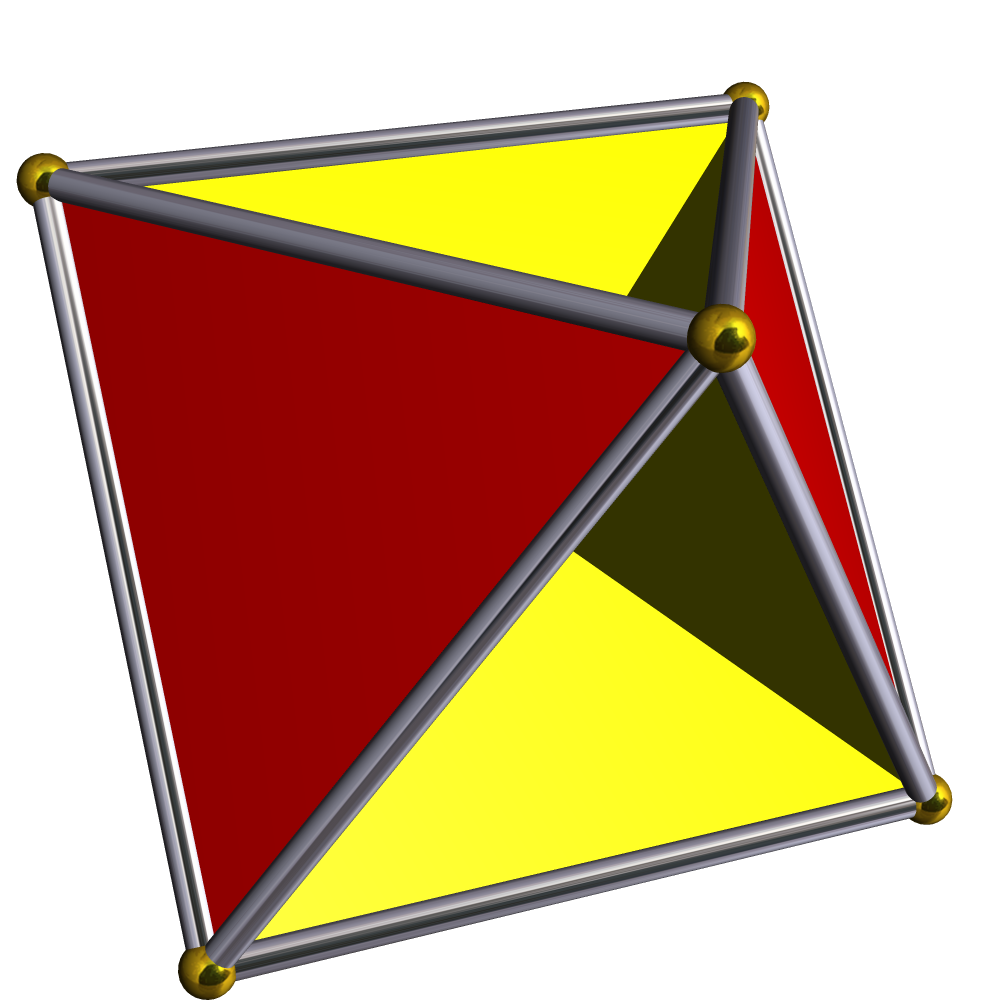
\includegraphics{Figures/Tetrahemihexahedron.png}
%https://en.wikipedia.org/wiki/Euler_characteristic#/media/File:Tetrahemihexahedron.png
\caption[Tetrahemihexaedro]{Tetrahemihexaedro regular. Algunas de sus caras se
intersecan entre sí, haciendo que su topología sea diferente a la de la bola
cerrada. Imagen: \cite{Tetra}.}
\end{marginfigure}

Un espacio topológico $X \subset \mb{R}^n$ 2AN y Hausdorff es una superficie
si, dado $p \in X$, existe un entorno abierto $U \subset X$ de $p$ homeomorfo
a una bola de $\mb{R}^2$. Desde un punto de vista geométrico, podemos decir
que los puntos de $X$ perciben el mundo en dos dimensiones, al igual que los
personajes de la novela \emph{Planilandia}. Algunas superficies pueden ser
representadas utilizando poliedros regulares, que podemos clasificar en
función de su característica de Euler. Cuando una superficie sea homeomorfa a
algún poliedro regular, diremos que es poliédrica.

A partir de un espacio topológico, podemos generar una familia de grupos
abelianos llamados \emph{grupos de homología}. Los grupos de homología nos
permiten utilizar técnicas de álgebra conmutativa para conocer algunas de las
propiedades topológicas de un espacio, permitiendo probar resultados que están
fuera del alcance de la topología conjuntista. En particular, veremos una
demostración del teorema del punto fijo de Brouwer, que establece la
existencia de puntos fijos para cualquier aplicación continua entre conjuntos
convexos.

Este texto está fuertemente basado en \cite{Vick94}, un texto dirigido a
estudiantes de máster y doctorado (conocido en Estados Unidos como el
\emph{graduate level}), por lo que las explicaciones son más breves y muchos
detalles se asumen triviales. Mi objetivo es adaptar estos textos, de
forma que sean lo más asequible posible a estudiantes de 3º y 4º de carrera.

Dado que la información en \cite{Vick94} está muy concentrada, se han tomado
los dos primeros capítulos y convertido en partes. Se recomienda al lector
tratar de entender y computar ejemplos antes de pasar a la parte siguiente.

La primera parte de este texto corresponde al capítulo 1, \emph{Singular
Homology Theory}, donde se introducen los grupos de homología singular y las
sucesiones de Mayer-Vietoris. Las sucesiones de Mayer-Vietoris son la técnica
básica para calcular los grupos de homología de un espacio topológico, y
son válidas para cualquier espacio.

La segunda parte corresponde al capítulo 2, \emph{Attaching Spaces with Maps},
donde se introducen los espacios CW-complejos y los grupos de homología
celular. La homología celular es una forma más directa de computar los grupos
de homología, pero requiere que nuestro espacio admita una estructura especial,
la \emph{estratificación por CW-complejos}.

Finalmente, los apéndices presentan información adicional que no es necesaria
para poder seguir el texto, pero he considerado interesante y digma de
discusión.

El objetivo de este texto es introducir al lector en la teoría de homología
singular, y está dirigido principalmente a estudiantes de la \emph{Universitat
de València}. Como consecuencia, el lector se asume familiarizado con el
contenido cubierto por las asignaturas de Estructuras algebraicas y Topología
de segundo curso.


\pagelayout{wide} % No margins
\addpart{Homología singular de un espacio topológico}
\pagelayout{margin} % Restore margins
\setchapterpreamble[u]{\margintoc}

\chapter{Grupos de homología singular}
\section{Símplices singulares}
Decimos que una familia de puntos $S=\{x_0, \dots, x_p\} \subset \mb{R}^n$ es \textbf{afínmente independiente} si, dados $\lambda_1,\dots,\lambda_n, \mu_1,\dots,\mu_n \in \mb{R}$ tales que
	\begin{align*}
		\sum^p_{i=0}\lambda_ix_i=\sum^p_{i=0}\mu_ix_i; && \sum^p_{i=0}\lambda_i=\sum^p_{i=0}\mu_i
	\end {align*}
se verifica que $\lambda_i=\mu_i$ para todo $1\leq i \leq n$.

\begin{proposition}
	La familia de puntos $S=\{x_0, \dots, x_p\} \subset \mb{R}^n$ es afínmente independiente si y sólo si la familia de vectores
		\[T=\{x_1-x_0,\dots,x_p-x_0\}\]
	es linealmente independiente.
\end{proposition}

\begin{proof}
	Supongamos que $S$ es afínmente independiente y sean $\lambda_1,\dots, \lambda_p$ tales que
	\begin{equation}\label{CombLinNula}
		\sum^p_{i=1}\lambda_i(x_i-x_0)=0 \iff \sum^p_{i=1}\lambda_ix_i=x_0\sum^p_{i=1}\lambda_i
	\end{equation}

Definimos $\lambda_0=-\lambda_1-\dots-\lambda_p$.
Por construcción, se verifica que $\lambda_0+\lambda_1+\dots+\lambda_p=\lambda_0-\lambda_0=0$.
Aplicando \eqref{CombLinNula},
	\[0=\sum^p_{i=1}\lambda_i(x_i-x_0)=\sum^p_{i=1}\lambda_i x_i-x_0\sum^p_{i=1}\lambda_i=\sum^p_{i=0}\lambda_i x_i\]

Por otro lado, también podemos escribir $0=0x_0+\dots+0x_p$.
Dado que $S$ es una familia afínmente independiente, $\lambda_i=0$ para todo $i=1,\dots,n$.
Por tanto, $T$ es linealmente independiente.

Recíprocamente, sean $T$ una familia linealmente independiente y $\mu_0,\alpha_0,\dots,\mu_p,\alpha_p \in \mb{R}$ tales que
\begin{align*}
	\sum_{i=0}^p \mu_ix_i=\sum_{i=0}^p \alpha_ix_i; && \sum_{i=0}^p \mu_i=\sum_{i=0}^p \alpha_i
\end{align*}
Combinando ambas igualdades, deducimos que
\begin{align*}
0=\sum^p_{i=0}(\mu_i-\alpha_i)x_i
	&=\sum^p_{i=0}(\mu_i-\alpha_i)x_i-0x_0=\\
	&=\sum^p_{i=0}(\mu_i-\alpha_i)x_i-
	\left(\sum^p_{i=0}(\mu_i-\alpha_i)\right)x_0=\\
	&=\sum^p_{i=1}(\mu_i-\alpha_i)(x_i-x_0)
\end{align*}

Dado que $T$ es linealmente independiente, se sigue que
	\[\mu_i-\alpha_i=0 \iff \mu_i=\alpha_i \quad (i=1,\dots, p)\]

Sabiendo que la suma de todos los $\mu_i$ es la misma que la de todos los $\alpha_i$, se sigue que $\mu_0=\alpha_0$.
Por tanto, $S$ es afínmente independiente.
\end{proof}

\begin{marginfigure}
\begin{tikzpicture}[scale=0.6]
%Puntos
\draw (3,3)[fill=black] circle (1pt);
\draw (3,3.5) node {$a$};

\draw (0,0)[fill=black] circle (1pt);
\draw (0,-.5) node {$b$};

\draw (-3,3)[fill=black] circle (1pt);
\draw (-3,3.5) node {$c$};

%Vectores
\draw[-to] (0,0) -- (1,1);
\draw[-to] (0,0) -- (-1,1);

%Líneas
\draw[dashed] (-1,-1) -- (4,4);
\draw (2,1.5) node {$L_1$};

\draw[dashed] (1,-1) -- (-4,4);
\draw (-2,1.5) node {$L_2$};
\end{tikzpicture}
\caption[Puntos afínmente independientes]{La independencia afín es una forma de definir independencia lineal en conjuntos afines, donde los elementos son puntos y no vectores.}
\end{marginfigure}

Sea $S \subset \mb{R}^n$ un conjunto afínmente independiente y $(a,b,c)$ una terna de elementos de $S$ con $a\neq b \neq c$.
Si $S$ es afínmente independiente, debe pasar que los vectores $a-b$ y $b-c$ sean linealmente independientes.

Como $a-b\neq 0$, existe una recta afín $L_1 \subset \mb{R}^n$ que tiene a $a-b$ como vector director.
De la misma forma, existe otra recta afín $L_2 \subset \mb{R}^n$ que tiene a $b-c$ como vector director.
Por independencia lineal, se tiene que $L_1$ no es paralelo a $L_2$, por lo que $a \not\in L_2$ y $c \not\in L_1$.

Por tanto, un conjunto afínmente independiente es aquel en el que no hay tres puntos colineales.

\begin{definition}
	Un \textbf{$p$-símplice} es la envoltura convexa de una familia de puntos $\{x_0, \dots,x_p\} \subset \mb{R}^n$ afínmente independientes.
	Dichos puntos reciben el nombre de \textbf{vértices} del símplice.
\end{definition}

\marginnote{
\begin{kaobox}[frametitle=Envoluta convexa]
Un $C \subseteq \mb{R}^n$ no vacío es convexo si, dados $x,y \in C$, $C$ contiene al segmento $[x,y]=\{xt+y(1-t)\colon t \in [0,1]\}$.
Si $A \subset \mb{R}^n$ es no vacío, se define su envoltura convexa como el menor subconjunto convexo que contiene a $A$,
	\[\con(A)=\bigcup_{x,y \in A}[x,y]\]
\end{kaobox}
}

Sea $A$ una familia de puntos afínmente independientes de $\mb{R}^n$ y
	\[i\colon \mb{R}^n \hookrightarrow \mb{R}^m\]
la inclusión.
Se tiene que $i(A)$ es una familia de puntos afínmente independiente de $\mb{R}^m$, por lo que los símplices de $\mb{R}^n$ son también símplices en $\mb{R}^m$.
Por tanto, no es necesario especificar dónde estamos considerando los símplices.

\begin{proposition}\labprop{BaseVertices}
	Sea $S\subset \mb{R}^n$ un $p$-símplice y $\{x_0,\dots x_p\}$ una familia afínmente independiente de puntos contenidos en $S$.
	Dado un punto $x \in S$, existe una familia única de escalares $t_0,\dots, t_p \in [0,1]$ tales que
	\begin{align*}
		x=\sum^p_{i=0}t_ix_i; && \sum^p_{i=0}t_i=1
	\end{align*}
	Por lo que una familia de vértices de un símplice es el equivalente a una base en un espacio vectorial.
\end{proposition}

Decimos que un $p$-símplice está \textbf{ordenado} cuando se aplica una relación de orden determinada sobre sus vértices.

\begin{example}
	Sean $a=(1,0,0)$, $b=(0,1,0)$ y $c=(0,0,1)$.
	La envoltura convexa de $\{a,b,c\}$ es un 2-símplice, que denotaremos como $\sigma$.
	Si $e_1=a$, $e_2=b$ y $e_3=c$, la relación de orden
		\[e_i \leq e_j \iff i \leq j\]
	hace que $\sigma$ sea un 2-símplice ordenado.
\end{example}

\begin{marginfigure}
\centering
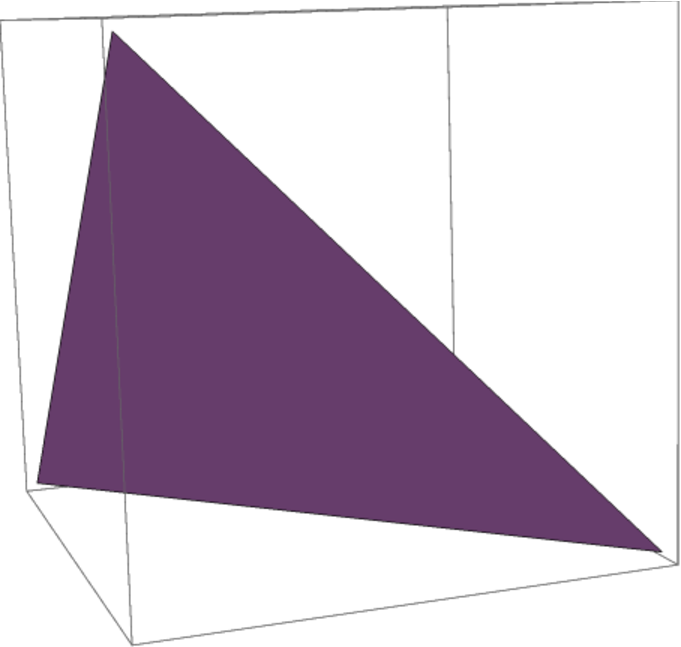
\includegraphics{2Simplice.pdf}
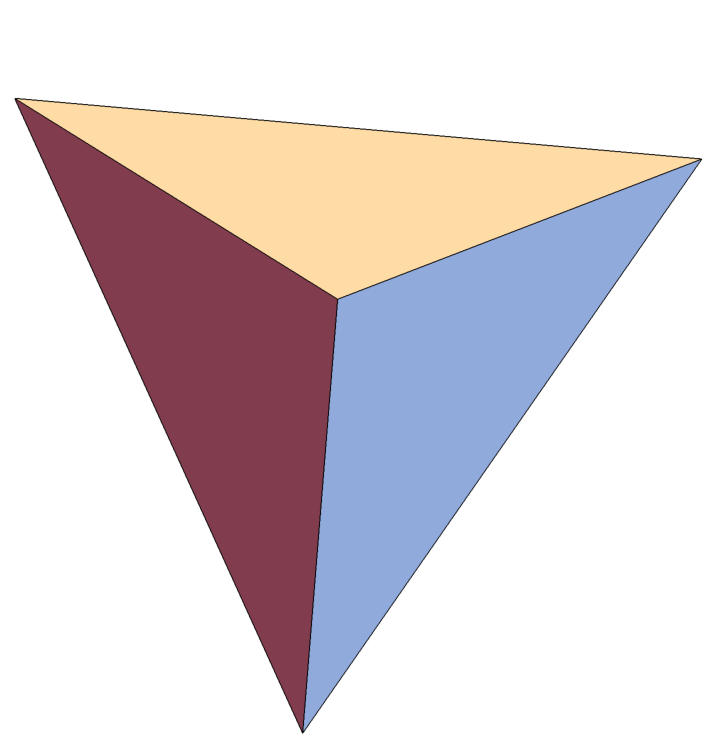
\includegraphics{Simplice.pdf}
\caption[Triángulo y tetraedro]{Los triángulos y tetraedros constituyen ejemplos de símplices. Podemos crear una teoría de homología utilizando sólo símplices, pero se limitaría a espacios topológicos contenidos en $\mb{R}^n$.}
\labfig{123Simplice}
\end{marginfigure}

Sea $\{e_1, \dots, e_{n+1}\}$ la base canónica de $\mb{R}^{n+1}$.
La envoltura convexa de los puntos $\{e_1, \dots, e_{n+1}\}$ es un $n$-símplice, que denotaremos como $\sigma_n$.
Por \refprop{BaseVertices}, los puntos de $\sigma_n$ son de la forma
\begin{align*}
	(t_1,\dots,t_{n+1}) \in \mb{R}^{n+1}; && t_1+\dots+t_{n+1}=1
\end{align*}

Sea $S=\{x_0,\dots,x_n\}\subset \mb{R}^m$ una familia de puntos afínmente independientes: la aplicación continua
\begin{funcion}
f\colon \sigma_n \arrow[r]                   & \con(S)            \\
{(t_0,\dots,t_n)} \arrow[r, maps to] & \displaystyle\sum^n_{i=0}t_ix_i
\end{funcion}
establece una biyección entre $\sigma_n$ y $\con(S)$.
Dado que $\sigma_n$ es compacto y $\con(S)$ es un espacio de Hausdorff, $f$ es un homeomorfismo, por lo que $\con(S)$ es homeomorfo a $\sigma_n$.

De la observación anterior, se sigue que todo $p$-símplice de $\mb{R}^{p+1}$ es homeomorfo a $\sigma_p$, por lo que podemos considerarlo como el representante canónico de todos los $p$-símplices.
En consecuencia, $\sigma_p$ recibe el nombre de \textbf{$p$-símplice estándar}.

\begin{example}
	\labexample{012simp}
	\begin{enumerate}
		\item El conjunto $\sigma_0$ es el singulete formado por el punto $1 \in \mb{R}$.
		\item El conjunto $\sigma_1$ es el segmento que une los puntos $(1,0)$ y $(0,1)$ de $\mb{R}^2$.
		\item El conjunto $\sigma_2$ es el triángulo de vértices $e_1, e_2, e_3 \in \mb{R}^3$. 
	\end{enumerate}
\end{example}

Si nos limitamos a subespacios topológicos en $\mb{R}^n$, podemos crear una teoría de homología utilizando sólo símplices (\sidecite{Lujan18}).
Sin embargo, si queremos definir una teoría que cubra todos los espacios topológicos, necesitamos transportar el símplice utilizando aplicaciones continuas.

\begin{definition}
Sea $X$ un espacio topológico.
Un \textbf{$p$-símplice singular} de $X$ es una aplicación continua
	\[\phi\colon \sigma_p \to X\]
\end{definition}

\begin{example}\labexample{S1Complejo}
Sea $\mb{D}=\{z \in \mb{C}: |z|=1\}$.
La aplicación
\begin{funcion}
	\phi\colon \sigma_1 \arrow[r]	& \mb{D}\\
	(t_0,t_1) \arrow[maps to,r] 	& e^{\pi i t_0}
\end{funcion}
es un símplice singular, que envía al 1-símplice estándar en la mitad superior del 1-símplice mostrado en \reffig{Circunferencia}.
Notemos que $\phi(\sigma_1)$ no es un segmento desde el punto de vista geométrico porque tiene curvatura no nula, pero sí lo es desde un punto de vista topológico, ya que $\phi$ es un homeomorfismo y $\sigma_1$ es un segmento.
\end{example}

\begin{marginfigure}
	\resizebox{\textwidth}{!}{
\begin{tikzpicture}[scale=0.8]
\draw [to-to] (-2.5,0) -- (2.5,0);
\draw [to-to] (0,-2.5) -- (0,2.5);

\draw[thick,dashed] (0,0) circle (2cm);

\draw[thick] (2,0) arc (0:180:2);
\draw (1,2.2) node {$\phi(\sigma_1)$};
\end{tikzpicture}
}
	\caption[Circunferencia]{La curva $\phi(\sigma_1)$ dada por el símplice singular $\phi$ de \refexample{S1Complejo}.
	Los símplices singulares amoldan el símplice estándar al espacio de llegada usando su continuidad.}
	\labfig{Circunferencia}
\end{marginfigure}

Dado un $p \in X$ y un espacio topológico $Y$, toda aplicación constante $\cte_p\colon Y \to X$ se identifica con el $0$-símplice singular $\phi_p\colon \sigma_0 \to X$ que envía al punto $1$ en $p$.
De la misma forma, si $I$ es un intervalo cerrado de $\mb{R}$, todo camino $\alpha\colon I \to X$ se identifica con el $1$-símplice singular
\begin{funcion}
\psi\colon	\sigma_1 \arrow[r]             & X            \\
		{(t_0,t_1)} \arrow[r, maps to] & \alpha(t_0)
\end{funcion}

Sean $X$, $Y$ espacios topológicos.
Dada una aplicación continua $f\colon X \to Y$ y un $p$-símplice singular $\phi\colon \sigma_p \to X$, la aplicación
	\[f_\#(\phi):=f\circ \phi\colon \sigma_p \to Y\]
es un $p$-símplice singular en $Y$ por ser composición de aplicaciones continuas.
Esto hace que toda aplicación continua dé lugar a una aplicación que envía $p$-símplices singulares de $X$ en $p$-símplices singulares de $Y$.

\begin{proposition}\labprop{ComposicionAlmohadilla}
	\begin{enumerate}
	\item Si $\id_X$ es la aplicación identidad, $(\id_X)_\#$ también es la aplicación identidad.
	\item Si $f\colon X \to Y$ y $g\colon Y \to Z$ son aplicaciones continuas,
		\[(g\circ f)_\#=g_\#\circ f_\#\]
	\end{enumerate}
\end{proposition}

Sea $X$ un espacio topológico, $\phi\colon \sigma_p \to X$ un $p$-símplice singular y $0 \leq i \leq p$.
Se define la \textbf{cara $i$-ésima de $\phi$} como el $(p-1)$-símplice singular
\begin{funcion}
	\p_{(i)}\phi\colon \sigma_{p-1} \arrow[r] & X \\
	{(t_0,\dots,t_{p-1})} \arrow[r, maps to] &
	\phi(t_0,\dots,t_{i-1},0,t_{i},\dots,t_{p-1})
\end{funcion}

\begin{example}
Considérese el 2-símplice singular
\begin{funcion}
	\phi\colon  \sigma_2 \arrow[r] & \mb{R}^3 \\
	(x,y,z) \arrow[r, maps to] & (2x+2,2y+2,2z+2)
\end{funcion}

Las caras de $\phi$ son los $1$-símplices singulares
\begin{align*}
\p_{(0)}\phi(u,v)=\phi(0,u,v)=(2,2u+2,2v+2)\\
\p_{(1)}\phi(u,v)=\phi(u,0,v)=(2u+2,2,2v+2)\\
\p_{(2)}\phi(u,v)=\phi(u,v,0)=(2u+2,2v+2,2)
\end{align*}

Desde un punto de vista geométrico, $\p_{(i)}\phi(\sigma_1)$ son las caras del tetraedro $\phi(\sigma_2)$ para $i=0,1,2$.
\end{example}

\section{Grupos libres}
Sea $G$ un grupo abeliano y $n \in \mb{Z}$ un entero no nulo.
Dado un $g \in G$, se define el producto $ng$ como
\begin{align*}
ng:=\sum^n_{j=0}g	&& ng:=\sum^{-n}_{j=0}-g\\
(n>0)				&& (n < 0)
\end{align*}
Si $n=0$, se considera que $0g=0$ para todo $g \in G$.

Decimos que un subconjunto $S \subset G$ es un \textbf{sistema generador} de $G$
si, dado un $g \in G$, podemos hallar $b_1,\dots,b_n \in S$ y enteros
$\mu_1,\dots,\mu_n$ tales que
\[g=\mu_1b_1+\mu_2b_2+\dots+\mu_nb_n\]

\begin{definition}
Sea $G$ un grupo abeliano. Un sistema generador $B$ de $G$ es una \textbf{base}
si, dados $b_1,\dots,b_n \in B$ y enteros $\lambda_1,\dots,\lambda_n$,
\begin{align}
\label{SisLibre} \sum^n_{i=1}\lambda_ib_i=0 \implies \lambda_i=0
\end{align}
Decimos que $G$ es un \textbf{grupo libre} si admite una base.
\end{definition}

\begin{example}
Supongamos que $\mb{Q}^+=(\mb{Q},+)$ es un grupo libre generado por un cierto
conjunto $B \subseteq \mb{Q}$. Dados $\frac{a}{b}, \frac{c}{d} \in B$, se tiene
que
\[cb\frac{a}{b}-ad\frac{c}{d}=0\]
por lo que $B$ está formado por un único elemento.

Sea $p$ un número primo coprimo con $b$. Por ser $\mb{Q}^+$ libre, existirá un
entero $\alpha$ tal que
\[\frac{1}{p}=\alpha\frac{a}{b}\]
pero esto implica que $b=\alpha pa$, en contradicción con la premisa de que $p$
es coprimo con $b$. Por tanto, $\mb{Q}^+$ no es un grupo libre.
\end{example}

\subsection{Grupo libre generado por un conjunto}
\marginnote[-2.2cm]{
\begin{kaobox}[frametitle=Aplicaciones nulas casi por todas partes]
Sea $A$ un conjunto no vacío. Decimos que una aplicación $f\colon A
\to \mb{Z}$ es \textbf{nula casi por todas partes} si podemos hallar un
subconjunto $B \subseteq A$ finito tal que $f(x)=0$ para todo
$x \in A\backslash B$.
\end{kaobox}
}
\begin{proposition}
Sea $A \neq\emptyset$. Se define el grupo libre generado por $A$ como la familia
$\mc{F}(A)$ de todas las aplicaciones $f\colon A \to \mb{Z}$ que se
hacen cero casi por todas partes. Entonces, $\mc{F}(A)$ es un grupo libre dotado
con la suma elemento a elemento.
\end{proposition}

\begin{proof}
Dado un $a \in A$, se define $\mc{X}_a\colon A \to \mb{Z}$ como
\[\mc{X}_a(x)=\begin{cases}
1&\mbox{ si }x=a\\
0&\mbox{ si }x\neq a
\end{cases}\]
Notar que $\mc{X}_a$ es una aplicación nula casi por todas partes, por lo que
$\mc{X}_a \in \mc{F}(A)$. La base de $\mc{F}(A)$ será el conjunto
\[X:=\{\mc{X}_a: a\in A\} \subseteq \mc{F}(A)\]

Dada una aplicación $f \in \mc{F}(A)$, se define $\tilde{f}$ como
\[\tilde{f}=\sum_{a \in A}f(a)\mc{X}_a\]
Dado un $x \in A$,
\begin{equation}
\label{tildef}\tilde{f}(x)=\sum_{a \in A} f(a)\mc{X}_a(x)=
f(x)\underbrace{\mc{X}_x(x)}_{=1}+
\sum_{a \neq x}f(a)\underbrace{\mc{X}_a(x)}_{=0}=f(x)
\end{equation}
por lo que $\tilde{f}=f$. Por tanto, toda aplicación de $\mc{F}(A)$ es
combinación lineal de elementos de $X$, de forma que $X$ es un sistema generador
de $\mc{F}(A)$.

Sean $\mu_1,\dots,\mu_n$ enteros y $a_1,\dots,a_n \in A$ tales que
$\mu_1\mc{X}_{a_1}+\dots+\mu_n\mc{X}_{a_n}=0$. Dado un $1 \leq j \leq n$,
\[0=\sum^n_{i=1}\mu_i\mc{X}_{a_i}(a_j)=
\mu_j\underbrace{\mc{X}_{a_j}(a_j)}_{=1}+
\sum^n_{i \neq j}\mu_i\underbrace{\mc{X}_{a_i}(a_j)}_{=0}=\mu_j\]
por lo que $\mu_1,\dots,\mu_n=0$. Por tanto, $X$ es una base.
\end{proof}

Por convenio, se considera que $\{0\}=\mc{F}(\emptyset)$.

\begin{example}
$\mc{F}(\mb{N})$ es el conjunto de todas las sucesiones $(a_n)_{n=1}^\infty$
de $\mb{Z}$ con $a_n=0$ para casi todo $n \in \mb{N}$. Es decir, el anillo de
polinomios sobre $\mb{Z}$.
\end{example}

Notar que, si $A=\{a_1,\dots,a_n\}$, la aplicación
\begin{funcion}
\Psi\colon \mc{F}(A) \arrow[r]	& \mb{Z}^n\\
f \arrow[maps to,r]			& (f(a_1),\dots,f(a_n))
\end{funcion}
es un isomorfismo de grupos.

\section{Complejos de cadenas}
\begin{definition}
Un \textbf{grupo graduado} es una colección de grupos $G=\{G_n: n \in \mb{Z}\}$.
Diremos que $G$ es \textbf{abeliano} si todos los grupos $G_n$ lo son.
\end{definition}

Sean $G,H$ grupos graduados. Un \textbf{homomorfismo graduado} $f\colon G
\rightarrow H$ es una colección de homomorfismos
\[f_i\colon G_i \to H_{i+r} \quad (i \in \mb{Z})\]
siendo $r \in \mb{Z}$ un valor común para todos los $f_i$. Dicho entero se
denomina \textbf{grado} de $f$.

\begin{definition}
Dos grupos graduados $G$, $H$ son \textbf{isomorfos} si, dado un entero $p$,
existe un isomorfismo $f_p\colon G_p \to H_p$. Al homomorfismo
graduado $f=\{f_p\}_{p \in \mb{Z}}$ se le denomina \textbf{isomorfismo graudado}.
\end{definition}

\marginnote[-2.2cm]{
\begin{kaobox}[frametitle=Subgrupo normal]
Un subgrupo $H \leq G$ es normal si, dados $g \in G$ y $n \in N$, $ng=gm$ para
algún $m \in N$. Esta condición es importante para poder garantizar que las
clases del espacio cociente están bien definidas, pero se puede obviar cuando
$G$ es abeliano.
\end{kaobox}
}

Si $G, H$ son grupos graduados, decimos que $H$ es un \textbf{subgrupo graduado}
de $G$ si, dado un entero $n$, $H_n \leq G_n$. En particular, si
$H_n$ es un subgrupo normal para todo $n$, se define el \textbf{grupo graduado
cociente} como
\[\frac{G}{H}:=\left\{\frac{G_i}{H_i}: i \in \mb{Z}\right\}\]

\begin{definition}
Un \textbf{complejo de cadenas} es un par de la forma $(G,\p)$, siendo $G$ un
grupo graduado y $\p$ un endomorfismo de grado -1 tal que
\[\im  \p_n \leq \ker \p_{n-1}\]
La aplicación $\p$ recibe el nombre de \textbf{operador borde}.
\end{definition}

Diremos que un complejo de cadenas $(C,d)$ es \textbf{abeliano} si lo es $C$.

\begin{definition}
Sean $(C,d)$ y $(C',d')$ dos complejos de cadenas. Una \textbf{aplicación de
cadenas} es un homomorfismo graduado $\Phi\colon C \to C'$ de grado
$0$ tal que el siguiente diagrama es conmutativo para todo $n$:
\begin{diagram}
C_{n+1} \arrow{r}{d_{n+1}} \arrow{d}{\Phi_{n+1}} & C_n \arrow{d}{\Phi_n} \\
C'_{n+1} \arrow{r}{d'_{n+1}}                     & C'_n                   
\end{diagram}
\end{definition}

\subsection{Grupo de homología asociado a un complejo de cadenas}
Sea $(C,d)$ un complejo de cadenas. Se definen los grupos graduados
\begin{align*}
Z_*(C)&:=\ker d=\{\ker d_n: n \in \mb{Z}\};	& Z_n(C)&:=\ker d_n\\[0.2cm]
B_*(C)&:=\im d=\{\im d_n: n \in \mb{Z}\}; 	& B_n(C)&:=\im d_n
\end{align*}
Diremos que dos elementos $p,q \in Z_n(C)$ son \textbf{homólogos} si
$p-q \in B_n(C)$.

\begin{definition}
Sea $C$ un complejo de cadenas. Se definen el \textbf{grupo graduado de
homología} y el \textbf{grupo de homología} de orden $n$ de $C$ como 
\begin{align*}
H_*(C):=\frac{Z_*(C)}{B_*(C)}; && H_n(C)=\frac{Z_n(C)}{B_n(C)}
\end{align*}
Diremos que dos complejos de cadenas tienen el mismo \textbf{tipo de homología}
si sus grupos de homología son isomorfos.
\end{definition}

Sea $f\colon (C,d) \to (D,\p)$ una aplicación de cadenas. Dado un
$c \in Z_n(C)$,
\[d_n(c)=0 \implies \p_n[f_n(c)]=f_{n-1}[d_n(c)]=f_{n-1}(0)\]
Como $f_{n-1}$ es un homomorfismo de grupos, $f_{n-1}(0)=0$, por lo que
$f_n(c)\in Z_n(D)$ y $f_n[Z_n(C)]\leq Z_n(D)$.

Análogamente, $f_n(B_n(C)) \leq B_n(D)$. Por tanto, $f$ induce un homomorfismo
entre grupos de homología,
\[f_*\colon H_*(C) \to H_*(D)\]

\subsection{El grupo de las cadenas singulares}
\begin{definition}
Se define el grupo de \textbf{$n$-cadenas
singulares} $S_n(X)$ como el grupo libre generado por todos los símplices
singulares $\phi\colon \sigma_n \to X$. Los elementos de $S_n(X)$
reciben el nombre de $n$-\emph{cadenas singulares} de $X$.
\end{definition}

A partir los grupos de cadenas singulares, podemos definir el grupo graduado
\[S_*(X)=\{S_n(X): n \geq 0\}\]
Para poder completar el grupo graduado, simplemente se considera que $S_p(X)=0$
para todo $p < 0$.

El objetivo de esta sección es definir un operador borde sobre $S_*(X)$, de
forma que $(S_*(X),\p)$ forme una complejo de cadenas. Podemos extender el
operador cara a $S_n(X)$ tomando
\[\p_{(j)}\left(\sum_{i=1}^n k_i\phi_i\right)= \sum^n_{i=1}k_i\,\p_{(j)}\phi_i\]
Este proceso da lugar a $n+1$ operadores cara diferentes, pero ninguno de ellos
define un operador borde.

\begin{definition}
Se define el \textbf{operador borde} $\p\colon S_n(X) \to
S_{n-1}(X)$ asociado a $S_*(X)$ como
\[\p=\sum^n_{j=0}(-1)^j\partial_{(j)}\]
\end{definition}

\begin{theorem}\labthm{OperadorBorde}
Dado un espacio topológico $X$, $\im \p \leq \ker \p$. Esto implica que $(S_*(X),
\p)$ es un complejo de cadenas.
\end{theorem}

\marginnote[-2.2cm]{
\begin{kaobox}[frametitle=Ejercicio]
Esta demostración se basa en la cuenta de la vieja, pero la naturaleza de los
operadores cara pueden hacerlo engorroso de seguir.
Antes de leer la prueba, intenta probarlo para $n=4$. Si puedes hacerlo sin
ayuda, puedes ignorar la prueba.
\end{kaobox}
}

\begin{proof}
Sea $c \in S_n(X)$. Dado que $S_n(X)$ es un grupo libre y $\p$ es un
homomorfismo, podemos suponer sin pérdida de generalidad que $c$ es un símplice
singular $\sigma_n \to X$.

Por definición de $\p$,
\begin{equation}
\label{Borde2c}
\p^2c=\sum^{n-1}_{p=0}(-1)^p\p_{(p)}(\p c)=
\sum^n_{q=0}\sum^{n-1}_{p=0}(-1)^{p+q}\p_{(p)}\p_{(q)}c
\end{equation}

Para continuar, necesitamos la siguiente identidad: dados $0 \leq p, q \leq n$
con $p < q-1$,

\begin{align*}
\p_{(p)}\p_{(q)}&c(t_0,\dots,t_{n-2})
	=\p_{(q)}c(t_0,\dots,t_{p-1},\stackrel{(p)}{0},t_p,\dots,t_{n-2})=\\
	&=c(t_0,\dots,t_{p-1},\stackrel{(p)}{0},t_p,\dots,t_{q-2},
	\stackrel{(q)}{0},t_{q-1},\dots,t_{n-2})=\\
	&=\p_{(p)}c(t_0,\dots,t_{q-2},\stackrel{(q-1)}{0},t_{q-1},\dots,t_{n-2})=\\[9pt]
	&=\p_{(q-1)}\p_{(p)}c(t_0,\dots,t_{n-2})
\end{align*}

Combinando ambas expresiones,
\begin{align*}
\p^2c
	&\stackrel{\eqref{Borde2c}}{=}
	\sum_{q=1}^n\sum_{p < q-1}(-1)^{p+q}\p_{(p)}\p_{(q)}c+
	\sum^n_{q=0}\sum_{p > q}(-1)^{p+q}\p_{(p)}\p_{(q)}c
\end{align*}

\begin{marginfigure}
\resizebox{\textwidth}{!}{
\begin{tikzpicture}[scale=.5]
%Región p > q
\filldraw[draw opacity=0, fill=red!30] (0,0) -- (5,5) -- (6,5) -- (6,0) -- cycle;
\draw[dashed] (0,0) -- (5,5);

\draw (0,5.5) -- (0,0) -- (6.5,0);
\draw (7,0) node {$q$};
\draw (0,6) node {$p$};

%q axis
\foreach \x in {0,...,4}
{
\draw (\x,-0.125) -- (\x,0.125);
\draw (\x,-0.5) node {$\x$};
}

\draw (5,-.5) node {$\dots$};

\draw (6,-0.125) -- (6,0.125);
\draw (6,-.5) node {$n$};

%p axis
\foreach \x in {0,...,3}
{
\draw (-0.125,\x) -- (0.125,\x);

\draw (-.5,\x) node {$\x$};
}

\draw (-.5,4) node {$\vdots$};

\draw (-0.125,5) -- (0.125,5);
\draw (-1,5) node {$n-1$};

\draw (4,2) node {$p > q$};
\end{tikzpicture}
}
\caption[Gráfica auxiliar que ilustra el cambio de índices.]{Gráfica auxiliar
para visualizar el cambio de índices descrito en la ecuación
\eqref{CambioIndices}.}
\end{marginfigure}
Obseremos que
\begin{multline} \label{CambioIndices}
\{(p,q)\colon q=0,\dots,n,\, 0\leq p<q\}=\\
\{(q,p)\colon p=0,\dots,n-1,\, p < q \leq n\}
\end{multline}
por lo que $\p^2c$ se puede escribir como
\begin{align*}
	&\sum_{q=1}^n\sum_{p < q-1}(-1)^{p+q}\p_{(q-1)}\p_{(p)}c+
	\sum^n_{q=0}\sum_{p < q}(-1)^{p+q}\p_{(p)}\p_{(q)}c=\\ 
	&=\sum_{q=0}^{n-1}\sum_{p < q}(-1)^{p+q+1}\p_{(q)}\p_{(p)}c+
	\sum^{n-1}_{p=0}\sum_{q > p}(-1)^{p+q}\p_{(q)}\p_{(p)}c=\\
	&=\sum_{q=0}^{n-1}\left(-\sum_{p < q}(-1)^{p+q}\p_{(q)}\p_{(p)}c+
	\sum_{p < q}(-1)^{p+q}\p_{(q)}\p_{(p)}c\right)=0
\end{align*}
\end{proof}

Dado que $S_*(X)$ es abeliano por definición, su grupo de homología asociado
está bien definido. Además, como todo espacio topológico $X$ define un grupo
graduado $S_*(X)$ de forma única, podemos introducir la siguiente notación sin
ambigüedades:
\begin{align*}
Z_n(X):=Z_n(S_*(X)); && B_n(X):=B_n(S_*(X))
\end{align*}

\begin{definition}
Sea $X$ un espacio topológico. Se define el \textbf{grupo de homología de orden
$n$ asociado a $X$} como
\[H_n(X):=H_n(S_*(X))=\frac{Z_n(X)}{B_n(X)}\]
\end{definition}

\begin{example}\labexample{Camino1ciclo}
Sea $f\colon [0,1] \to X$ un camino. Se define el 1-símplice singular
\begin{funcion}
\psi\colon \sigma_1 \arrow[r] & X\\
(t_0,t_1) \arrow[r,maps to] & f(t_0)
\end{funcion}
Se tiene entonces que $\psi$ es un 1-ciclo si y sólo si
\[\p \psi=0 \iff \psi(0,1)=\p_{(0)}\psi=\p_{(1)}\psi=\psi(1,0)\]
Dado que $\psi(0,1)=f(0)$ y $\psi(1,0)=f(1)$, un camino es un 1-ciclo si y sólo
si $f$ es un lazo.
\end{example}

\subsection{Morfismo inducido en homología}
Sea $f\colon X \to Y$ una aplicación continua. Habíamos definido una
aplicación $f_\#$ que convierte símplices de $X$ en símplices de $Y$, al igual
que el operador cara convertía $n$-símplices en $(n-1)$-símplices. Podemos extender $f_\#$ a todo el grupo de cadenas singulares de forma que la
aplicación resultante sea un homomorfismo:
\[f_\#\left(\sum^k_{j=1}n_j\phi_j\right)=\sum^k_{j=1}n_jf_\#(\phi_j)\]
Esta aplicación recibe el nombre de \textbf{morfismo inducido en homología} por
$f$.

\begin{proposition}
Todo morfismo inducido por una aplicación continua es una aplicación de cadenas.
Como consecuencia, si $f\colon X \to Y$ es continua, $f_\#$ induce
una familia de homomorfismos
\begin{funcion}
f_*: H_n(X) \arrow[r] &H_n(Y)\\
\left[x\right] \arrow[maps to,r]    &\left[f_\#(x)\right]
\end{funcion}
para $n \geq 0$.
\end{proposition}

Dadas $f\colon X \to Y$ y
$g\colon Y \to Z$ continuas, deducimos de \refprop{ComposicionAlmohadilla} y de este resultado que
\[(g\circ f)_*=g_*\circ f_*\]
Por tanto, deducimos que los grupos de homología son invariantes topológicos:

\begin{theorem}
Sean $X,Y$ espacios topológicos. Si $f\colon X \to Y$ es un homeomorfismo, $f_*\colon H_k(X) \to H_k(Y)$ es un isomorfismo para todo $k \geq 0$. Por tanto, el
grupo de homología es un invariante topológico.
\end{theorem}

\section{Interpretación geométrica de los grupos de homología}
Sea $X=\mb{R}^2\backslash\{(0,0)\}$ con la topología inducida por $\mb{R}^2$. El
espacio $\mb{R}^2$ no es homeomorfo a $X$; sin embargo, no es posible probar
este resultado utilizando sólo topología conjuntista. En esta sección, veremos
cómo la teoría de homología nos permite probar que no existe un homeomorfismo
entre $\mb{R}^2$ y $X$.

Definimos un \textbf{camino orientado} en un espacio topológico $X$ como una
terna $(\gamma; A,B)$, siendo $\gamma\colon [0,1] \to X$ un camino
con $\gamma(0)\neq \gamma(1)$ y $A,B \in \gamma(\{0,1\})$ con $A\neq B$. Diremos
que $(\gamma; A,B)$ está \textbf{orientado positivamente} (resp.
\textbf{negativamente}) si $A=\gamma(0)$ y $B=\gamma(1)$.

\begin{example}
Sea $\eta\colon [0,1] \to \mb{R}^2$ el camino dado por
\[\eta(t)=(\sin(\pi t),-\cos(\pi t))\]
La orientación negativa de $\eta$ (que podemos ver en
\reffig{MotivHomologia}) viene dada por $A=\eta(1)=(0,1)$ y $B=\eta(0)=(0,-1)$.
\end{example}

\marginnote[-2.2cm]{
\begin{kaobox}[frametitle=Caminos compatibles]
Diremos que dos caminos orientados $(\alpha;A_1,B_1)$ y $(\beta;A_2,B_2)$ en $X$
son \textbf{compatibles} si el camino $\gamma\colon [0,1] \to X$
dado por
\[\gamma(t)=
\begin{cases}
\alpha(2t) & 0 \leq t \leq \frac{1}{2}\\
\beta(2t-1) & \frac{1}{2} \leq t \leq 1
\end{cases}\]
es continuo y $B_1=A_2$.
Por ejemplo, los caminos $\phi$ y $\eta$ de \reffig{MotivHomologia} son compatibles.
\end{kaobox}
}

Consideremos los siguientes caminos positivamente orientados en $\mb{R}^2$:
\begin{align*}
\eta(t)	&=(\sin(\pi t),-\cos(\pi t)); &&\phi(t)=(\cos(\pi t),\sin(\pi t));\\
\mu(t)	&=(2\sin(\pi t),-\cos(\pi t));
\end{align*}

Los caminos $\phi$ y $\eta$ tienen orientaciones compatibles, y forman una
circunferencia cuyo interior está contenido en $\mb{R}^2$. Por tanto, podemos
hallar una cadena singular cuyo borde sea $\phi+\eta$. Si tomamos clases módulo
$B_1(\mb{R}^2)$,
\[\phi+\eta \in B_1(\mb{R}^2) \iff -[\eta]=[\phi]\]

Los caminos $\eta$ y $\mu$ forman una figura homotópica a una circunferencia, y
sus orientaciones son compatibles. Podemos encontrar una cadena singular cuyo
borde sea $\phi+\mu$. Tomando clases,
\[\phi+\mu \in B_1(\mb{R}^2) \iff [\phi]=-[\mu]\]

\begin{marginfigure}
\resizebox{\textwidth}{!}{
\begin{tikzpicture}
\draw[thick] (0,0) circle (2cm);
\draw (0,0) node {$\star$};

\draw[fill=black] (0,2) circle (1.5pt);
\draw (0,2.5) node {$A$};

\draw [-stealth] (2,0) -- (2,1);
\draw (2.5,0.5) node {$\eta$};

\draw[fill=black] (0,-2) circle (1.5pt);
\draw (0,-2.5) node {$B$};

\draw [-stealth] (-2,0) -- (-2,-1);
\draw (-2.5,-0.5) node {$\phi$};

%Primera distancia -> Eje horizontal
%Segunda distancia -> Eje vertical
\draw[thick] (0,2) arc (90:-90:4cm and 2cm);

\draw [-stealth] (4,0) -- (4,-1);
\draw (4.5,-0.5) node {$\mu$};
\end{tikzpicture}
}
\caption{Varios caminos en $\mb{R}^2$.\labfig{MotivHomologia}}
\end{marginfigure}

Consieremos ahora el plano perforado, $X=\mb{R}^2\backslash\{(0,0)\}$. La
aplicación $\phi|_X+\eta|_X$ ya no forma el borde de una cadena singular, dado
que los caminos encierran al punto $(0,0)$, que no está. Por tanto, las clases
de $\phi|_X$ y $\mu|_X$ serán diferentes. En cambio, $\phi$ y $\psi$ siguen
siendo homólogas, porque sus orientaciones son compatibles y no contienen al
punto que hemos quitado.

Dado que el grupo de homología es un invariante topológico, concluimos que
$\mb{R}^2$ no es homeomorfo a $X$.

\section{Característica de Euler}
\begin{definition}
Sea $A$ un grupo abeliano. Se denomina \textbf{subgrupo de torsión} de $A$ al
subgrupo $T$ formado por todos los elementos de orden finito de $A$. Decimos que
$A$ es \textbf{libre de torsión} si $T=0$, y que $A$ es un \textbf{grupo de
torsión} si $T=A$.
\end{definition}

Si $T$ es el subgrupo de torsión de un cierto grupo abeliano $A$,
$A/T$ es un grupo libre de torsión.

\begin{example}
\begin{enumerate}
\item El grupo aditivo $\mb{Z}_n=\mb{Z}/n\mb{Z}$ es un grupo de torsión: dado un $\overline{p} \in
\mb{Z}_n$,
\[n\overline{p}=\sum^{n|p|}_{i=1}\overline{1}=\sum^{|p|}_{i=1}\overline{n}=
\sum^{|p|}_{i=1}0=0\]
Por la misma razón, todo cuerpo de característica mayor que cero define un grupo de torsión.
\item El grupo aditivo $\mb{Z}$ es un grupo libre de torsión porque no tiene divisores de cero: si $n > 0$ y $p \in \mb{Z}$ es tal que $np=0$, necesariamente se cumple que $p=0$.
\end{enumerate}
\end{example}

\begin{example}
Consideremos el grupo $\mb{Z}\times \mb{Z}_n$. Dado un $\overline{q} \in \mb{Z}_n$,
\[n(0,\overline{q})=\sum^n_{i=1}(0,\overline{q})=(0,n\overline{q})=(0,0)\]
por lo que el subgrupo de torsión de $\mb{Z}\times \mb{Z}_n$ contiene a
$\{0\}\times\mb{Z}_n$. Sin embargo, si $m > 0$ y $p \in \mb{Z}$,
\[m(p,\overline{q})=\sum^m_{i=1}(p,\overline{q})=(mp,m\overline{q})=(0,0)\]
Ésto es tanto como decir que $n$ divide a $mq$ y $p=0$. Por tanto, el subgrupo
de torsión de $\mb{Z}\times \mb{Z}_n$ es $\{0\}\times\mb{Z}_n$.
\end{example}

Sea $A$ un grupo abeliano y $T$ el subgrupo de torsión de $A$, que es un
subgrupo normal por ser $A$ abeliano. Se define el \textbf{rango} de $A$ como el
mínimo número de generadores que posee $A/T$.

\begin{definition}
Sea $X$ un espacio topológico. Se define el \textbf{$n$-ésimo número de Betti}
$\beta_n(X)$ como el rango de $H_n(X)$. Si existe un $k \in \mb{N}$ tal que
$\beta_p(X)=0$ para todo $p > k$, se define la \textbf{característica de Euler}
de $X$ como 
\[\mc{X}(X):=\sum^k_{n=0}(-1)^n\beta_n(X)\]
\end{definition}

\setchapterpreamble[u]{\margintoc}

\section{Homología de un espacio arcoconexo}
Sea $X$ un espacio topológico arcoconexo.
Dados dos puntos $x,y \in X$, existe un camino $L_{x,y}\colon [0,1] \to X$ tal que $L_{x,y}(0)=x$ y $L_{x,y}(1)=y$.
Como vimos en \refexample{Camino1ciclo}, $L_{x,y}$ induce un $1$-símplice singular $\phi\colon \sigma_1 \to X$.
En particular, $L_{x,x}=\cte_x$ es una aplicación constante que queda totalmente determinada por $x$, por lo que podemos identificar $x$ con $L_{x,y}$.

Dado que $\cte_x \in S_0(X)$, existirán $x_1,\dots,x_n \in X$ y enteros $\mu_1,\dots,\mu_n$ tales que
\[x \equiv \cte_x=\sum^n_{i=1}\mu_i\cte_{x_i} \equiv \sum^n_{i=1}\mu_ix_i\]

Consideremos el último tramo del complejo de cadenas $S_*(X)$:
\begin{diagram}
	S_1(X) \arrow{r}{\p_1} & S_0(X) \arrow{r}{\p_0} & 0
\end{diagram}
Dado que $\p_0=0$, $S_0(X)=Z_0(X)$ y podemos construir el siguiente homomorfismo entre $S_0(X)$ y $\mb{Z}$:
\begin{funcion}
	\beta\colon S_0(X) \arrow{r}           & \mb{Z}          \\
	n_1x_1+\dots+n_px_p \arrow[r, maps to] & n_1+\dots+n_p
\end{funcion}
Como $X\neq\emptyset$, $\beta$ es epimorfismo, ya que $p=\beta(px)$ para todo $x \in X$.

Sea $\phi \in S_1(X)$: como $\p$ es un homomorfismo de grado $-1$, $\p\phi \in S_0(X)$.
En particular, $\phi$ es una aplicación continua que depende de dos variables no negativas, $t_0$ y $t_1$, cuya suma siempre es 1.
Si computamos el operador borde,
\begin{align*}
	\p\phi			&=\phi(0,t_0)-\phi(t_0,0)=\phi(0,1)-\phi(1,0);\\
	\beta(\p\phi)	&=\beta(\phi(0,1)-\phi(1,0))=1-1=0,
\end{align*}
por lo que $\p\phi \in \ker\beta$.
Si $c=n_1\phi_1+\dots+n_p\phi_p$,
	\[\beta(\p c)=
		\beta(n_1\p\phi_1+\dots+n_p\phi_p)=
		n_1\beta(\p\phi_1)+\dots+n_p\beta(\p\phi_p)=0\]
Pero $\p c$ son los elementos de $B_0(X)$, por lo que $B_0(X) \subseteq\ker \beta$.

Recíprocamente, sea $c \in \ker \beta$: identificando cada punto con la aplicación constante que lleva a todo el espacio en ese punto, existirán $x_1,\dots,x_k \in X$ tales que $c=n_1x_1+\dots+n_kx_k$.
Como $X$ es arcoconexo, dado un $x \in X$, podemos construir la cadena singular $d=n_1L_{x,x_1}+\dots+n_kL_{x,x_k}$ y
	\[\p d=
		\sum^p_{i=1}n_i(L_{x,x_i}(1)-L_{x,x_i}(0))=
		\sum^k_{i=1}n_ix_i-x\sum^k_{i=1}n_i.\]
Como $c \in \ker \beta$, se sigue que
	\[\sum^p_{i=1}n_i=\beta(c)=0 \implies \p d=\sum^p_{i=1}n_ix_i=c.\]

\marginnote[-2.2cm]{
	\begin{kaobox}[frametitle=Teorema de isomorfía]
		Dado un homomorfismo $f\colon G \to H$,
			\[\im f\cong \frac{G}{\ker f}\]
	\end{kaobox}
}

Por tanto, $c \in B_0(X)$ y $B_0(X)=\ker \beta$.
Aplicando el teorema de isomorfía,
	\[H_0(X)=\frac{Z_0(X)}{B_0(X)}=\frac{S_0(X)}{\ker \beta} \cong \mb{Z}\]

\begin{proposition}
	Sea $X$ un espacio topológico arcoconexo.
	El grupo $H_0(X)$ tiene un único generador.
\end{proposition}

\begin{example}
Sea $X=\{\star\}$.
Dado un $n \geq 0$, existe un único $n$-símplice singular $\phi_n\colon\sigma_n \to X$, que es la aplicación constante.
Las caras de la aplicación constante son la aplicación constante, por lo que
\begin{align*}
\p\phi_n=
	\begin{cases}
	\phi_{n-1}	&\mbox{ si }n\mbox{ es par}\\
	0          	&\mbox{ si }n\mbox{ es impar}
	\end{cases}
\end{align*}

Dado que $S_n(X)=\la \phi_n\ra$, el operador borde $\p_n\colon S_n(X) \to S_{n-1}(X)$ es un isomorfismo si $n$ es par y cero si $n$ es impar.
Por tanto, $H_n(X)=0$ para todo $n > 0$ y $H_0(X)\cong \mb{Z}$.
\end{example}

\subsection{Sumas directas en homología}
Sea $\{G_\alpha\}_{\alpha \in A}$ una familia de grupos abelianos.
Se define el \textbf{producto directo} de los grupos $G_\alpha$ como el grupo
\[G=\prod_{\alpha \in A} G_\alpha:=
	\left\{\left.f\colon A \to \bigcup_{\alpha \in A}G_\alpha\,\right|f(\alpha) \in G_\alpha \quad \forall \alpha \in A\right\}\]
Denotaremos a las aplicaciones $f \in G$ como tuplas de la forma $f=(f_\alpha)_{\alpha \in A}=\{f(\alpha)\}_{\alpha \in A}$
Los elementos $f_\alpha$ reciben el nombre de \textbf{componentes} de $f$.

\begin{example}\labexample{SumaDirectaZ}
Sea $A=\{0,\dots, n\}$. El producto directo
\[G=\prod_{\alpha \in A}\mb{Z}\]
es isomorfo al subgrupo de $\mb{Z}[x]$ formado por polinomios de grado menor
o igual que $n$, por lo que podemos identificar $f \in G$ con un polinomio
\[f(x)=f_0+f_1x+f_2x^2+\dots+f_nx^{n}\]

Tomando $A=\mb{N}$, $G$ es isomorfo al grupo aditivo $\mb{Z}[x]$. Sin embargo,
también podemos verlo como el grupo de sucesiones en $\mb{Z}$ junto con la suma.
\end{example}

\begin{definition}\labdef{SumaDirecta}
Sea $\{G_\alpha\}_{\alpha \in A}$ una familia de grupos abelianos con producto
directo $G$. Se define la \textbf{suma directa} de $\{G_\alpha\}_{\alpha \in A}$
como el subgrupo $H$ de $G$ formado por las aplicaciones nulas casi por todas
partes.
\end{definition}

Cuando consideramos una familia finita de grupos abelianos, no hace falta
distinguir entre la suma y el producto directo. La diferencia entre las sumas y
los productos directos sólo se manifiesta cuando consideramos una familia
infinita:

Una serie de potencias sobre $\mb{Z}$ se define como una suma formal de la forma
\begin{equation}
f(x)=\sum^\infty_{j=0}f_jx^j \quad (f_j \in \mb{Z}) \label{SeriePotencias}
\end{equation}
La familia de todas las series de potencias sobre $\mb{Z}$ se denota como
$\mb{Z}[[x]]$.

Podemos ver $\mb{Z}[[x]]$ como el producto directo de $\mb{Z}$ consigo mismo una
cantidad numerable de veces. Es claro que $\mb{Z}[x]$ es un subgrupo de
$\mb{Z}[[x]]$: la suma formal \eqref{SeriePotencias} es un polinomio si y sólo si
$f_j=0$ para todo $j$ mayor que un cierto $j_0$. Sin embargo, no todas las series
de potencias son polinomios: no existe ningún polinomio que sea igual a
\begin{equation}
\sum^\infty_{n=0}x^n=\frac{1}{1-x} \label{UnoMenosX}
\end{equation}

Como consecuencia de esta inclusión estricta, $\mb{Z}[x]$ tiene propiedades que
$\mb{Z}[[x]]$ no cumple. Por ejemplo, todo elemento de $\mb{Z}[x]$ da lugar a una
función $f\colon \mb{Q} \to \mb{Z}$, pero la suma formal \eqref{UnoMenosX} diverge
en la topología estándar de $\mb{Q}$ cuando $x \geq 1$.

Dada una familia de complejos de cadenas $\{C^\alpha\}_{\alpha \in A}$, se define
el grupo graduado
\[C=\sum_{\alpha \in A}C^\alpha:=
\left\{\sum_{\alpha \in A}C^\alpha_p:\; p \in \mb{Z}\right\}\]

Dado un $c \in C_p$, existen $\alpha_1,\dots,\alpha_n \in A$ tales que
$c(\alpha)=0$ para todo $\alpha \in A\backslash \{\alpha_1,\dots,\alpha_n\}$.
Podemos entonces identificar $c$ con un elemento
$(c^{\alpha_1},\dots,c^{\alpha_n}) \in
C^{\alpha_1}_p\oplus\dots\oplus C^{\alpha_n}_p$. Si denotamos al operador borde
de $C^{\alpha_j}$ como $\p^{\alpha_j}$,
\[\left(\p^{\alpha_1}_pc^{\alpha_1},\dots,\p^{\alpha_n}_pc^{\alpha_n}\right) \in
C^{\alpha_1}_{p-1}\oplus\dots\oplus C^{\alpha_n}_{p-1}\]
Por tanto, definimos la siguiente aplicación:
\begin{diagram}
\p_p\colon C_p \arrow[r]             & C_{p-1}                   \\[-8mm]
c \arrow[r, maps to] &
(\p^{\alpha_1}_pc^{\alpha_1}_p,\dots,\p^{\alpha_n}c^{\alpha_n}_p)
\end{diagram}
Dado que $\p_p$ actúa componente a componente, es inmediato que esta construcción
da lugar a un operador borde.

\begin{lemma}\lablemma{HomoSumaDir}
Dada una familia de complejos de cadenas $\{C^\alpha\}_{\alpha \in A}$ con suma
directa $C$,
\[H_*(C)\cong\sum_{\alpha \in A}H_*(C^\alpha)\]
\end{lemma}

\subsection{Descomposición en arcocomponentes}
Supongamos $\Omega$ es un espacio topológico formado por dos arcocomponentes,
$\Omega_1$ y $\Omega_2$, como los que se muestran en \reffig{FigPentaHexa}. Si
$f(x) \in \Omega_1$, por continuidad, $f(\sigma_p) \subseteq \Omega_1$. De esta
forma, todos los elementos de la base de $H_p(\Omega)$ están en $H_p(\Omega_1)$ o
en $H_p(\Omega_2)$; es decir,
\[H_p(\Omega)\cong H_p(\Omega_1)\oplus H_p(\Omega_2)\]

\begin{marginfigure}
\resizebox{\textwidth}{!}{
\begin{tikzpicture}
\draw[fill=blue, fill opacity=0.5] (-1,-1) circle (1cm);
\draw (-2,0) node {$\Omega_1$};

\draw[thick] (-1,-1) arc (15:114:0.5);

\draw[fill=green, fill opacity=0.5] (1,1) circle (1cm);
\draw (0,2) node {$\Omega_2$};

\draw[thick] (1,1) arc (0:95:0.5);

\draw[thick, dashed] (-1,-1) -- (1,1);
\end{tikzpicture}
}
\caption[Dos espacios arcoconexos, cada uno conteniendo la imagen de un
símplice singular, junto con una línea discontinua que sale de uno de ellos
para entrar en el otro.]{\labfig{FigPentaHexa}Los arcos de circunferencia son
$1$-símplices singulares de $\Omega$, pero la línea discontinua uniéndolos no
lo es, ya que se sale del espacio.}
\end{marginfigure}

\begin{proposition}
\labprop{SumaDirArco} Sea $X$ un espacio topológico y $\{X_\alpha\colon \alpha
\in A\}$ la familia de arcocomponentes de $X$.
\[H_*(X) \cong \sum_{\alpha \in A} H_*(X_\alpha)\]
\end{proposition}

\begin{proof}
Considérese la aplicación
\begin{diagram}
\Psi_k\colon\sum_\alpha S_k(X_\alpha) \arrow[r] & S_k(X)          \\[-0.8cm]
(g_\alpha)_\alpha \arrow[r, maps to]            & \sum_\alpha g_\alpha
\end{diagram}

Toda cadena singular $g \in S_k(X)$ admite una descomposición única como
combinación lineal de $k$-símplices singulares. Dado que cada símplice va a parar
a una única componente conexa de $X$, se sigue que
\[\Psi_k(g)=\Psi_k(h) \implies g=h\]
por lo que $\Psi_k$ es inyectiva.

Sea $\phi\colon \sigma_k \to X$ un $k$-símplice singular. Las aplicaciones
continuas preservan la arcoconexión, por lo que $\phi(\sigma_k)$ está en alguna
componente arcoconexa $X_\alpha \subseteq X$. Por tanto, podemos hallar un
$\phi_\alpha \in S_k(X_\alpha)$ tal que
\[\Psi_k(\phi_\alpha)=\phi\]
por lo que $\Psi_k$ es sobreyectiva.

Dado $g=(g_\alpha)_\alpha$,
\[\Psi_k(\p g)=
\Psi_k({\p^\alpha g_\alpha})=
\sum_{\alpha \in A}\p^\alpha g_\alpha=
\p \sum_{\alpha \in A}g_\alpha=\p \Psi_k(g)\]
Se sigue que $\Psi$ es aplicación de cadenas y
\[H_*(X)=H_*[S_*(X)]\cong H_*\left[\sum_{\alpha \in A}S_*(X_\alpha)\right]\]

Finalmente, aplicando \reflemma{HomoSumaDir},
\[H_*\left[\sum_{\alpha \in A}S_*(X_\alpha)\right]\cong
\sum_{\alpha \in A}H_*[S_*(X_\alpha)]=
\sum_{\alpha \in A}H_*\left(X_\alpha\right)\]
\end{proof}
Como consecuencia de este resultado, podemos asumir que todo espacio topológico es
arcoconexo.

Sea $X_\alpha$ una arcocomponente de $X$ y $x,y \in Z_0(X_\alpha)$. Si $a,b \in
\mb{Z}$, $ax+by \in Z_0(X_\alpha)$. Teniendo en cuenta que
\[ax+by=ax+ay-ay+by=a(x-y)+y(a+b)\]
siendo $x-y$ el borde de un 1-símplice y $a+b$ un entero, se tiene que
\[[ax+by]=[a(x-y)+y(a+b)]=a[x-y]+(a+b)[y]=(a+b)[y]\]
Es decir,
\[H_0(X_\alpha)=\la [y]\ra \cong \mb{Z}\]
Si $X$ tiene $n$ arcocomponentes, existirán $y_i \in H_0(X_i)$ ($1 \leq i \leq n$) tales que
\[H_0(X)=\sum^n_{\alpha=1}\la [y_\alpha]\ra\cong
\sum^n_{i=1}\mb{Z} \cong \mb{Z}^n\]

\begin{corollary}
Si $X$ tiene $n$ arcocomponentes,
\[H_0(X)\cong \mb{Z}^n\]
\end{corollary}

\subsection{Homología de un conjunto convexo}
El objetivo de este apartado es probar que todo conjunto convexo tiene el tipo de
homología de un punto. Es decir: si $X$ es un espacio convexo,
\begin{align*}
H_0(X)\cong \mb{Z}; && H_p(X)=0 \quad (p > 0)
\end{align*}
Ya sabemos que $H_0(X)$ tiene un único generador. Por tanto, nos queda probar la
segunda igualdad.

\begin{lemma}\lablemma{ConvexoLema}
Sea $X$ un conjunto convexo. Dado un símplice singular $\phi\colon \sigma_{p} \to
X$, la aplicación $T_p(\phi)\colon \sigma_{p+1} \to X$ dada por
\[(t_0,\dots,t_{p+1})\mapsto
\begin{cases}
\displaystyle(1-t_0)
\phi\left(\frac{t_1}{1-t_0},\dots,\frac{t_{p+1}}{1-t_0}\right)+t_0x
&\mbox{ si }t_0 < 1\\
x & \mbox{ si }t_0=1
\end{cases}\]
es un símplice singular.
\end{lemma}

\begin{proof}
Veamos primero que $T_p(\phi)$ está bien definida: si $t_0 < 1$,
\begin{equation}\label{BienDef}
\sum^{p+1}_{j=0}t_j=
1 \iff \sum^{p+1}_{j=1}t_j=
1-t_0 \iff \sum^{p+1}_{j=1}\frac{t_j}{1-t_0}=1
\end{equation}
por lo que los puntos de la forma $\frac{t_j}{1-t_0}$ están en $\sigma_p$ y
$T_p(\phi)$ está bien definida.

Sea $\tau_j=\frac{t_j}{1-t_0}$. La aplicación $T_p(\phi)$ es claramente continua
en todos los puntos con $t_0 < 1$ por ser composición de funciones continuas.
Pasemos al caso $t_0=1$:
\begin{multline*}
0	\leq \|T_p(\phi)(t_0,\dots,t_{p+1})-x\|=
\|(1-t_0)\phi(\tau_1,\dots,\tau_{p+1})-(1-t_0)x\|\leq\\
	\leq (1-t_0)(\|\phi(\tau_1,\dots,\tau_{p+1})\|+\|x\|)
\end{multline*}

Dado que $\phi$ es continua y $\sigma_p$ es compacto, $\phi(\sigma_p)$ es un
subconjunto compacto de $\mb{R}^n$, por lo que está acotado. Podemos encontrar un
$M > 0$ tal que $\|\phi(\tau_1,\dots,\tau_{p+1})\|$, por lo que
\[0 \leq \|T_p(\phi)(t_0,\dots,t_{p+1})-x\| \leq (1-t_0)(M+\|x\|)\]
De estas desigualdades, concluimos que
\[\lim_{t_0 \to 1}T_p(\phi)(t_0,\dots,t_{p+1})=x\]
y $T_p(\phi)$ es un símplice singular.
\end{proof}

\begin{theorem}\labthm{Convexo}
Sea $X \subset \mb{R}^n$ un conjunto convexo. Dado un $p > 0$,
\[H_p(X)=0\]
\end{theorem}

\begin{proof}
Dado un $p$-símplice singular $\phi$, sea $T_p(\phi)$ el símplice definido en el
lema \reflemma{ConvexoLema}. Queremos ver que
\begin{equation}
\phi=\p T_p(\phi)+T_p(\p \phi) \label{IdTp}
\end{equation}

Por un lado, $\p T_p(\phi)(t_0,\dots,t_p)=\phi(t_0,\dots,t_p)$ por lo que
$\p\circ T_p$ es la identidad. Por otro lado, dado $i=1,\dots,p+1$,
\begin{align*}
T_p(\p_{(i-1)}\phi)(t_0,\dots,t_p)
	&=(1-t_0)(\p_{(i-1)}\phi)(\tau_1,\dots,\tau_p)+t_0x=\\
	&=(1-t_0)\,\phi(\tau_1,\dots,\tau_{i-1},0,\tau_{i-1},\dots,\tau_p)+t_0x=\\
	&=T_p(\phi)(t_0,\dots,t_{i-1},0,t_i,\dots,t_p)=\\
	&=\p_{(i)}T_p(\phi)(t_0,\dots,t_p)
\end{align*}
de forma que $\p_{(i)}(T_p\phi)=T_p(\p_{(i-1)}\phi)$. Combinando ambas
identidades,
\begin{align*}
\p T(\phi)
	&=\p_{(0)}T(\phi)+\sum^{p+1}_{i=1}(-1)^i\partial_{(i)}(T_p\phi)=\\
	&=\phi+\sum^p_{i=0}(-1)^{i+1}T_p(\p_{(i)}\phi)=
	\phi-\sum^p_{i=0}(-1)^iT_p(\p_{(i)}\phi)
\end{align*}
de donde se sigue la identidad deseada.

Sea $z \in Z_p(X)$. Usando \eqref{IdTp}, $z=\p T_p(z)+T_p(\p z)=\p T_p(z)$,
por lo que $z \in B_p(X)$ y
\[H_p(X)=\frac{B_p(X)}{B_p(X)}=0\]
\end{proof}

\section{Homotopías en el grupo de homología}\labsec{HomoHomo}
\begin{definition}
Sea $X$ un espacio topológico. Decimos que $X$ es \textbf{contráctil} si existe
un punto $p \in X$ y una homotopía $F_p$ tal que
\[F_p\colon \id_X \simeq \cte_p\]
\end{definition}

Sea $X$ un espacio contráctil. Por definición, existe un punto $p \in X$ y una
homotopía $F\colon X \times [0,1] \to X$ tales que $F\colon \id_X \simeq
\cte_p$. Si ahora consideramos dos puntos $x,y \in X$, podemos construir el
camino $\alpha\colon [0,1] \to X$ dado por
\[\alpha(t)=
\begin{cases}
F(x,2t) & \text{ si $t < 1/2$}\\
F(y,1-2t) & \text{ si $t \geq 1/2$}
\end{cases}\]

Observamos que $F(x,1)=p=F(y,1)$, de forma que $\alpha$ es continua en
$t=1/2$. Por tanto, podemos hallar un camino que conecta todo par de puntos en
$X$, de forma que $X$ es arcoconexo.

\begin{example}
Sea $A \subseteq \mb{R}^n$ un conjunto convexo. Por ser convexo, dado un $a \in
A$, el segmento $[0,a]$ está contenido en $A$. Eso nos permite definir la
aplicación continua
\begin{diagram}
F\colon A\times I \arrow[r] & A                      \\[-0.8cm]
(a,t) \arrow[r, maps to]      & (1-t)a
\end{diagram}
por lo que $F\colon \id_A \simeq \cte_0$
\end{example}

\begin{marginfigure}
\resizebox{\textwidth}{!}{
\begin{tikzpicture}
\draw (0,4) -- (0,0) -- (3.5,0);

\foreach \x in {1,...,15}
{
\draw (3.5/\x,4) -- (3.5/\x,0);
}

\draw (3.5,-.35) node {$(1,0)$};
\draw (3.5/2,-.35) node {$(\frac{1}{2},0)$};
\draw (3.5/4,-.35) node {$\hdots$};
\draw (0,-.35) node {$(0,0)$};

\draw (3.5,4.35) node {$(1,1)$};
\draw (3.5/2,4.35) node {$(\frac{1}{2},1)$};
\draw (3.5/4,4.35) node {$\hdots$};
\draw (0,4.25) node {$(0,1)$};
\end{tikzpicture}
}
\caption[Peine del topólogo.]{\labfig{Peine} Primeras $15$ iteraciones del
peine del topólogo. La iteración $w$ añade el segmento correspondiente a
$x=1/w$.}
\end{marginfigure}

\begin{example}
Sea $\Sh$ (pronunciado \emph{sh}) el peine del topólogo. Consideremos la
aplicación continua
\begin{diagram}
F\colon \Sh\times I \arrow[r]             & \Sh                   \\[-8mm]
(x,y,t) \arrow[r, maps to] & (x,(1-t)y)
\end{diagram}
y la proyección sobre el eje de abscisas, $\pi\colon \mb{R}^2 \to \mb{R}$. La
aplicación $F$ es una homotopía que baja las púas de $\Sh$:
\[F: \id_\Sh \simeq (\pi\times \cte_0)\]
Dado que $\pi \simeq \cte_{(1,0)}$, $\Sh$ es un espacio contráctil.
\end{example}

\begin{definition}
Un subespacio $A$ de $X$ es un \textbf{retracto débil} si podemos hallar una
aplicación continua $r\colon X \to A$ tal que $r|_A\simeq \id_A$. Si podemos
construir $r$ de forma que $r|_A=\id_A$, decimos que $A$ es un \textbf{retracto
fuerte} (o simplemente \textbf{retracto}) y $r$ es una \textbf{retracción}.
\end{definition}

Sea $A$ un retracto de $X$ y $r\colon X \to A$ una retracción. Por definición de
retracto, si $i\colon A \hookrightarrow X$ es la inclusión,
\[r\circ i=\id_A \implies \id_{H_n(A)}=(1_A)_*=(r\circ i)_*=r_*\circ i_*\]
por lo que $r_*$ es sobreyectiva e $i_*$ es inyectiva.

\begin{example}
Sea $D^2$ la bola de centro $p=(0,0)$ y radio 1 de $\mb{R}^2$. Se considera la
aplicación
\begin{diagram}
r\colon D^2-\{p\} \arrow[r]             & S^1                   \\[-8mm]
x \arrow[r, maps to] & \frac{x}{\|x\|}
\end{diagram}
La aplicación $r$ es continua por ser cociente de funciones continuas. Además,
$r|_{S^1}=\id_{S^1}$. Se sigue que $S^1$ es un retracto de $D^2-\{p\}$.
\end{example}

\begin{example}[\cite{Spanier66}, p. 28]
Sea $X=[0,1]\times[0,1]$ el cuadrado unidad en $\mb{R}^2$. La inclusión $i\colon
\Sh \hookrightarrow X$ define un retracto débil. Sin embargo, se puede probar que
$\Sh$ no es un retracto fuerte de $X$.
\end{example}

\begin{definition}
Sea $A$ un subespacio de $X$. Decimos que $X$ es \textbf{deformable} en $A$ si
existe una aplicación continua $r\colon X \to A$ llamada \textbf{deformación} tal
que $i\circ r \simeq \id_X$, siendo $i\colon A \hookrightarrow X$ la inclusión.
\end{definition}

Dado que $i\circ r\simeq \id_X$, $i_*$ es sobreyectiva y $r_*$ es inyectiva.

\begin{example}\labexample{Deformacion}
\begin{enumerate}
\item Sea $\pi\colon \mb{R}^2 \to \mb{R}$ la proyección sobre el eje de abscisas.
Tomando la aplicación $r(t)=(\cos(2\pi t),\sin(2\pi t))$, se tiene que $r\circ
\pi\colon D^2 \to S^1$ es una deformación. No obstante, si tomamos el punto
$(0,1) \in S^1$,
\[(r\circ \pi)(0,1)=r(0)=(\cos 0,\sin 0)=(1,0)\neq (0,1)\]
por lo que $r\circ \pi$ no es una retracción.
\item Sea $X$ un espacio contráctil a un cierto punto $q$. Si $A$ es un
subespacio de $X$ que contiene a $q$, se tiene que $\cte_q\colon X \to A$ es
una deformación de $X$ en $A$ por definición de espacio contráctil. Por tanto,
$X$ es deformable en cualquier subespacio que contenga a $q$.
\end{enumerate}
\end{example}

\begin{definition}
Decimos que un subespacio $A$ es un \textbf{retracto por deformación fuerte} de
$X$ si podemos hallar una homotopía $F\colon X\times I \to X$ tal que 
\begin{enumerate}
\item dado un $x \in X$, $F(x,0)=x$;
\item $F(X,1) \subseteq A$;
\item dado un $a \in A$ y un $t \in I$, $F(a,t)=a$.
\end{enumerate}
\end{definition}

En particular, observamos que un retracto por deformación fuerte describe
tanto una deformación (ítem 2) como una retracción (ítem 3).

\begin{example}
El peine del topólogo no es un retracto por deformación fuerte del cuadrado
unidad, ya que no es un retracto fuerte.
\end{example}

Sea $i\colon A \hookrightarrow X$ la inclusión. Si $A$ es un retracto por
deformación de $X$, $X$ es deformable en $A$ ($i_*$ es un epimorfismo), pero
$A$ es un retracto de $X$ ($i_*$ es un monomorfismo). Por tanto, se tiene el
siguiente corolario:

\begin{corollary}\label{RDFHomo}
Los retractos por deformación fuerte no alteran el tipo de homología de un
espacio topológico.
\end{corollary}

\subsection{Homotopías de cadenas}
Sean $C$ y $D$ complejos de cadenas, con $f,g\colon C \to D$ aplicaciones de
cadenas. Queremos hallar una condición suficiente para poder afirmar que $f$ y $g$
inducen el mismo homomorfismo entre $H_p(C)$ y $H_p(D)$. Una forma de comprobar
esto es verificar que la aplicación de cadenas $\alpha=f-g\colon C \to D$ induce
el homomorfismo nulo en homologías:
\[f_*=g_* \iff \alpha_*=f_*-g_*=0\]

Sea $c \in Z_p(C) \leq C_p$. Supongamos que existe un $b \in D_{p+1}$ tal que
$\alpha(c)=\p b$. Por cómo se define $B_p(D)$, es inmediato que
\[\alpha_*([c])=[\p b]=0+B_p(D)\]
Existirá una homomorfismo $S\colon C_p \to D_{p+1}$ tal que $\alpha=\p \circ S$.
Pero esta no es una aplicación de cadenas, por lo que no sabemos si va a inducir
un homomorfismo entre los grupos de homología.

Como $S$ es un homomorfismo, $S(0)=0$; así, si tomamos $T=S|_{Z_p(C)}$, se
verifica que $\alpha=\p \circ T + T \circ \p$. Veamos que esta nueva definición
de $\alpha$ conmuta con el operador borde:
\begin{align*}
\p \circ \alpha &=
\p^2 \circ T+\p \circ T \circ \p =
\p \circ T \circ \p=\\
&=\p \circ T \circ \p + T \circ \p^2 =
\alpha \circ \p
\end{align*}

Por construcción, $\alpha_*$ es el homomorfismo nulo. Pero $\alpha=f-g$, por lo
que hemos encontrado una condición suficiente para que $f$ y $g$ induzcan el
mismo homomorfismo entre grupos de homología.

\begin{definition}
Sean $C$ y $D$ complejos de cadenas. Dos aplicaciones de cadenas
$f,g\colon C \to D$ son \textbf{homotópicas} si existe un homomorfismo $T\colon
C \to D$ de grado 1 tal que
\[f-g=\p \circ T+T\circ \p\]
La aplicación $T$ recibe el nombre de \textbf{homotopía de cadenas} entre $f$ y
$g$.
\end{definition}

\subsection{Aplicaciones homotópicas}
\begin{theorem}[Teorema de invarianza homotópica de la homología]
Dadas dos aplicaciones continuas $f,g\colon X \to Y$ homotópicas, $f_*=g_*$.
\end{theorem}

\begin{proof}
Sea $F\colon X \times I \to Y$ una homotopía entre $f$ y $g$. Se definen las
aplicaciones $\alpha,\beta\colon X \to X\times I$ dadas por las expresiones
\begin{align*}
\alpha(x)=(x,0); && \beta(x)=(x,1)
\end{align*}
de forma que $f=F\circ \alpha$ y $g=F\circ \beta$.

Supongamos que existe una homotopía de cadenas $T\colon S_*(X) \to
S_*(X\times I)$ entre $\alpha$ y $\beta$. $T$ induce una homotopía de cadenas
entre $f_\#$ y $g_\#$ de la siguiente forma:
\begin{align*}
f_\#-g_\#&=F_\#\circ\alpha_\#-F_\#\circ\beta_\#=
	F_\#\circ(\alpha_\#-\beta_\#)=\\
	&=F_\#\circ(\p \circ T+T\circ\p)=
	(F_\#\circ\p)\circ T+(F_\#\circ T)\circ\p
\end{align*}
Como $F_\#$ es una aplicación de cadenas,
\begin{align*}
(F_\#\circ\p)\circ T+(F_\#\circ T)\circ\p&=
(\p\circ F_\#)\circ T+(F_\#\circ T)\circ\p=\\
&=\p\circ (F_\#\circ T)+(F_\#\circ T)\circ\p
\end{align*}
por lo que $f_*=g_*$, que es lo que queríamos probar. Por tanto, bastará con
probar que $T$ existe.

Sea $\tau_n\colon \sigma_n \to\sigma_n$ la aplicación identidad. Procedemos a
construir $T$ de forma inductiva: supongamos que $X=\sigma_0$. El símplice
$\sigma_0$ es el espacio puntual formado por el punto 1, de forma que definimos
la 0-cadena
\[c=\alpha_\#(\tau_0)-\beta_\#(\tau_0)=\alpha-\beta \in S_0(\sigma_0\times I)\]
Como $S_0(\sigma_0\times I)=Z_0(\sigma_0\times I)$, $c$ es un 0-ciclo.

Dado que $\sigma_0$ es un espacio puntual, podemos identificar $\alpha$ con
$\alpha(1)=(1,0)$ y $\beta$ con $\beta(1)=(1,1)$. Como $\sigma_0\times I$ es
arcoconexo, existe un camino
\[b\colon I \to \sigma_0\times I\]
tal que $b(0)=(1,0)\equiv \alpha$ y $b(1)=(1,1)\equiv\beta$. Se sigue que $c=
\p b$. Definimos entonces $T_{\sigma_0}(\tau_0):=b$.

Si $X$ es un espacio topológico arbitrario y $\phi\colon \sigma_0 \to X$ un
0-símplice singular, definimos
\[T_X(\phi):=(\phi \times \id_I)_\#(T_{\sigma_0}(\tau_0))\]
La aplicación $T_X$ induce un homomorfismo de $S_0(X)$ en $S_1(X\times I)$ de
forma única.

Sea $X$ un espacio topológico arbitrario y $n > 0$. Supongamos construida para
todo $i < n$ una aplicación $T_X: S_i(X) \to S_{i+1}(X\times I)$ que verifique las
siguientes condiciones:
\begin{enumerate}
\item $\p\circ T_X+T_X\circ\p=\alpha_\#-\beta_\#$ ($\star$) \label{AlfaBetaHomo},
\item $T_X\circ h_\#=(h_\#\times 1_I)\circ T_X$ para toda aplicación continua
$h\colon X \to Y$.
\end{enumerate}

Dado un $d \in S_n(\sigma_n)$, $\p d \in S_{n-1}(\sigma_n)$, por lo que la cadena
singular
\begin{equation}
c=\alpha_\#(d)-\beta_\#(d)-T_{\sigma_n}(\p d)\label{PasoInductivo}
\end{equation}
está bien definida por hipótesis de inducción. Si calculamos $\p c$,
\begin{align*}
\p c&=\p\alpha_\#(d)-\p\beta_\#(d)-\p T_{\sigma_n}(\p d)
\stackrel{\hyperref[AlfaBetaHomo]{(\star)}}{=}\\
	&=\p\alpha_\#(d)-\p\beta_\#(d)-\p\alpha_\#(d)+\p\beta_\#(d)+
	T_{\sigma_n}(\p^2 d)=0
\end{align*}
por lo que $c \in Z_n(\sigma_n\times I)$. Dado que $\sigma_n\times I$ es convexo,
\[H_n(\sigma_n\times I)=
	0 \iff Z_n(\sigma_n\times I)=
	B_n(\sigma_n\times I)\]
por lo que $c \in B_n(\sigma_n\times I)$ Existirá entonces un $b \in
S_{n+1}(\sigma_n\times I)$ tal que $\p b=c$. Se define $T_{\sigma_n}(d)=b$.

Al igual que hicimos en el caso $n=0$, definimos
\[T_X(\phi)=(\phi\times \id_I)_\#(T_{\sigma_n}(\tau_n))\]
Nos queda ver que $T_X$ verifica las dos condiciones descritas en la hipótesis de
inducción.

Veamos que $T_{\sigma_n}$ verifica la condición
$\hyperref[AlfaBetaHomo]{(\star)}$:
\begin{align*}
\p T_{\sigma_n}(d)+T_{\sigma_n}(\p d)&=
\p b+T_{\sigma_n}(\p d)=
c+T_{\sigma_n}(\p d)
\stackrel{\eqref{PasoInductivo}}{=}\\
&=\alpha_\#(d)-\beta_\#(d)-
T_{\sigma_n}(\p d)+T_{\sigma_n}(\p d)=\\
&=\alpha_\#(d)-\beta_\#(d)
\end{align*}
Como la elección de $d$ es arbitraria, se deduce que
$\p\circ T_{\sigma_n}+T_{\sigma_n}\circ\p=\alpha_\#-\beta_\#$.

Sea $\phi\colon \sigma_p \to X$ un $p$-símplice singular. Antes de probar la
primera condición, notar que $\phi_\#(\tau_n)=\phi\circ\tau_n=\phi$, por lo que
\begin{equation}
(T_X\circ\phi_\#)(\tau_n)=T_X(\phi)=(\phi\times 1_I)_\#T_{\sigma_n}(\tau_n)
\label{TConmutaTau}
\end{equation}
De esta forma,
\begin{align*}
\p T_X(\phi)+T_X(\p \phi)
	&=[\p\circ (\phi\times \id_I)_\#\circ T_{\sigma_n}](\tau_n)+
	(T_X\circ\p\circ\phi_\#)(\tau_n)=\\
	&=[\p\circ(\phi\times \id_I)_\#\circ T_{\sigma_n}](\tau_n)+
	(T_X\circ \phi_\#)(\p\tau_n)\stackrel{\eqref{TConmutaTau}}{=}\\[8pt]
	&=[\p\circ(\phi\times \id_I)_\#\circ T_{\sigma_n}](\tau_n)+
	[(\phi\times 1_I)_\#\circ T_{\sigma_n}](\p\tau_n)=\\[8pt]
	&=[(\phi\times \id_I)_\#\circ\p\circ T_{\sigma_n}](\tau_n)+
	[(\phi\times 1_I)_\#\circ T_{\sigma_n}](\p\tau_n)=\\
	&=[(\phi\times \id_I)_\#\circ(\p\circ T_{\sigma_n}+
	T_{\sigma_n}\circ\p)](\tau_n)
	\stackrel{\hyperref[AlfaBetaHomo]{(\star)}}{=}\\[8pt]
	&=(\phi\times \id_I)_\#(\alpha_\#-\beta_\#)(\tau_n)
\end{align*}
Observamos que los diagramas
\begin{center}
\begin{minipage}{0.4\textwidth}
\begin{diagram}
\sigma_n \arrow{d}{\phi} \arrow{r}{\alpha} &
\sigma_n\times I \arrow{d}{\phi\times \id_I}\\
X \arrow{r}{\alpha}& X\times I&
\end{diagram}
\end{minipage}
%
\begin{minipage}{0.4\textwidth}
\begin{diagram}
\sigma_n \arrow{d}{\phi} \arrow{r}{\beta} &
\sigma_n\times I \arrow{d}{\phi\times \id_I}\\
X \arrow{r}{\beta}& X\times I&
\end{diagram}
\end{minipage}
\end{center}
son conmutativos, por lo que también conmutan cuando los
convertimos en aplicaciones de cadenas. De aquí se sigue que
\[[(\phi\times \id_I)_\#\circ(\alpha_\#-\beta_\#)](\tau_n)=
[(\alpha_\#-\beta_\#)\circ\phi_\#](\tau_n)=(\alpha_\#-\beta_\#)(\phi)\]
por lo que $\p\circ T_X+T_X\circ\p=\alpha_\#-\beta_\#$.

Para la segunda condición, consideramos $h\colon X \to W$ continua y $\phi \in
S_n(X)$:
\begin{align*}
T_W[h_\#(\phi)]&=
	(T_W \circ h_\#\circ \phi_\#) (\tau_n)=
	[T_W\circ(h\circ \phi)_\#](\tau_n)\stackrel{\eqref{TConmutaTau}}{=}\\[8pt]
	&=[(h\circ\phi)\times \id_I]_\#[T_{\sigma_n}(\tau_n)]=\\[8pt]
	&=[(h\times \id_I)\circ(\phi\times \id_I)]_\#[T_{\sigma_n}(\tau_n)]=\\
	&=[(h\times \id_I)_\#\circ(\phi\times \id_I)_\#][T_{\sigma_n}(\tau_n)]
	\stackrel{\eqref{TConmutaTau}}{=}\\[8pt]
	&=(h\times 1_I)[T_X(\phi)]
\end{align*}
por lo que se cumple la segunda condición.

De esta forma, se construye una homotopía de cadenas entre $\alpha$ y $\beta$.
\end{proof}

Sea $f\colon X \to Y$ una aplicación continua. Decimos que $f$ es una
\textbf{equivalencia de homotopía} si existe una aplicación $g\colon Y \to X$,
llamada \textbf{inversa homotópica}, tal que
\begin{align*}
f\circ g \simeq 1_Y; && g \circ f \simeq 1_X
\end{align*}

\begin{corollary}\label{Contractil}
Si $f\colon X \to Y$ es una equivalencia de homotopía,
\[f_*: H_*(X) \to H_*(Y)\]
es un isomorfismo de grado 0. En particular, si $X$ es un espacio contráctil,
\[H_n(X)\cong H_n(\{\star\})\cong
\begin{cases}
\mb{Z} 	& \text{ si $n=0$}\\
0		& \text{ si $n \neq 0$}
\end{cases}\]
\end{corollary}

\section{Sucesiones exactas}
\begin{definition}
Una colección de grupos y homomorfismos
\[G_0 \xrightarrow{ f_1 } G_1 \xrightarrow{ f_2 } G_2 \xrightarrow{ f_3 }
\dots \xrightarrow{ f_n } G_n\]
es una \textbf{sucesión exacta finita} si $\im f_j=\ker f_{j+1}$ para todo $j$.
\end{definition}

Si $n=4$ y $G_0=0=G_4$, se obtiene una sucesión exacta finita de la forma
\[0 \rightarrow G_1 \xrightarrow{ f_2 } G_2
\xrightarrow{ f_3 } G_3 \rightarrow 0\]
En este caso, hablamos de \textbf{sucesión exacta corta}. Notar que, por
definición de sucesión exacta, $f_2$ es un monomorfismo (su núcleo es el grupo 0)
y $f_3$ es un epimorfismo (su imagen es todo $G_3$).

\begin{definition}
Una colección de grupos y homomorfismos
\[G_0 \xrightarrow{ f_1 } G_1 \xrightarrow{ f_2 } G_2
\xrightarrow{ f_3 } \dots \xrightarrow{ f_n } G_n \xrightarrow{f_{n+1}} \dots\]
es una \textbf{sucesión exacta larga} si $\im f_j=\ker f_{j+1}$ para todo $j$.
\end{definition}

Sean $C,D,E$ complejos de cadenas. Considérese la sucesión exacta corta
\begin{equation}
0 \to C \xrightarrow{ f } D \xrightarrow{ g } E \to 0 \label{SecExactafg}
\end{equation}
siendo $f$ y $g$ aplicaciones de cadenas de grado 0. Por ser aplicaciones de
cadenas, dado un $p \geq 0$, podemos construir el diagrama
\[H_p(C) \xrightarrow{ f_* } H_p(D) \xrightarrow{ g_* } H_p(E)\]
Esta secuencia no es extacta, ya que $f_*$ (resp. $g_*$) podría no ser inyectiva
(resp. sobreyectiva). Lo que sí se cumple es que $\im f_*=\ker g_*$.

Para ver esta identidad, sea $c \in Z_p(C)$. Usando que \eqref{SecExactafg} es
una secuencia exacta,
\[(g\circ f)_*([c])=[(g\circ f)(c)]=0\]
por lo que $\im f_* \leq \ker g_*$.

Análogamente, sea $[z] \in \ker g_* \leq H_p(D)$. Sabemos que $[g(z)]=0$, por
lo que $g(z)=\p d$ para algún $d \in D_{p+1}$. Como $g\colon D_{p+1} \to
E_{p+1}$ es sobreyectivo, podemos hallar un $y \in D_{p+1}$ tal que $d=g(y)$.
Dado que $g$ es aplicación de cadenas,
\[g(z)=\p d=\p g(y)=g(\p y) \implies z-\p y \in \ker g\]

Usando $\ker g=\im f$, existirá un $x \in C_p$ tal que $z-\p y=f(x)$. Como
$[z] \in H_p(D)$, $z \in Z_p(D)$, luego
\[f(\p x)=\p f(x)=\p z-\p^2 y=0 \implies \p x \in \ker f\]
Pero $f$ es un monomorfismo, luego $\p x =0$ y $x \in Z_p(C)$. Esto nos permite
tomar clases módulo $B_p(C)$: usando $f(x)=z-\p y$,
\[f_*([x])=[z-\p y]=[z]\]

Por tanto, $[z] \in \im f_*$, luego $\ker g_* \leq \im f_*$.

Para poder generar una sucesión exacta larga, vamos a introducir un homomorfismo
$\Delta\colon H_*(E) \to H_*(C)$ (llamado \textbf{homomorfismo de conexión}) que
nos permita conectar $H_n(D)$ con $H_{n-1}(C)$. El resultado será una secuencia
exacta
\[\dots \xrightarrow{\Delta} H_n(C) \xrightarrow{ f_* } H_n(D) \xrightarrow{ g_* } H_n(E)
\xrightarrow{ \Delta } H_{n-1}(C)\xrightarrow{f_*}\dots\]

Sea $z \in Z_n(E)$. Como $g\colon D \to E$ es un epimorfismo de grado 0, existe
un $d \in D_n$ tal que $z=g(d)$. Como $z\in \ker \p$ y $g$ es aplicación de
cadenas,
\[g(\p d)=0 \implies \p d \in \ker g=\im f\]
A su vez, $f\colon C \to D$ es un homomorfismo de grado 0. Existirá un $c \in
C_{n-1}$ tal que $\p d=f(c)$. Pero $f$ es aplicación de cadenas inyectiva, por
lo que
\[0=\p d=\p f(c)=f(\p c) \implies c \in \ker f=0 \implies c \in Z_{n-1}(C)\]
Esto define una correspondencia $\delta\colon z \mapsto c$ que depende
implícitamente de $d$.

\begin{proposition}
La aplicación $\Delta\colon H_*(Z) \longrightarrow H_*(C)$ dada por
$\Delta([z])=[\delta c]$ está bien definida y es un homomorfismo.
\end{proposition}

\begin{proof}
Sean $z,z' \in Z_n(E)$ con $z-z' \in B_n(E)$. Existe un $e \in E_{n+1}$ tal que
$\p e=z-z'$.

Sean $d,d' \in D_n$ tales que $g(d)=z$ y $g(d')=z'$, y sean $c,c' \in C_n$ tales
que $\p d=f(c)$ y $\p d'=f(c')$. Dado que $g$ es un epimorfismo, existe un
$a \in D_{n+1}$ tal que $g(a)=e$. Como $g$ es aplicación de cadenas,
\[g(\p a)=\p e=z-z'=g(d-d')\]
de donde se sigue que $d-d'-\p a\in \ker g=\im f$. Podemos elegir entonces un
$b \in C_n$ tal que $f(b)=d-d'-\p a$. Usando que $f$ es aplicación de cadenas,
\[f(\p b)=\p(d-d'-\p a)=\p (d- d')=f(c-c')\]
por lo que $\p b-c-c'\in\ker f$.

Usando que $f$ es inyectiva, concluimos que $c-c'=\p b \in B_{n-1}(C)$.
\end{proof}

\begin{theorem}\labthm{SucExacHomo}
Sean $C, D, E$ complejos de cadenas y
\[0 \to C \xrightarrow{ f } D \xrightarrow{ g } E \to 0\]
una sucesión exacta corta. Si $\Delta\colon H_*(E) \to H_*(C)$ es un homomorfismo
de conexión,
\[H_n(C) \xrightarrow{ f_* } H_n(D) \xrightarrow{ g_* } H_n(E)
\xrightarrow{ \Delta } H_{n-1}(C)\] es una sucesión exacta larga.
\end{theorem}

\begin{proof}
La demostración consiste en dos pasos: probar que $\im g_*=\ker \Delta$ y que
$\im \Delta = \ker f_*$. Empecemos por la primera igualdad: dado un $[z] \in \im
g_*$, existe un $d \in Z_n(D)$ tal que $[g(d)]=[z]$. Dado que $g$ es aplicación
de cadenas y $z$ es un $n$-ciclo,
\[0=\p z=g(\p d) \implies \p d \in \ker g_*=\im f_*\]
Existirá un $c \in C_{n-1}$ de forma que $\p d=f(c)$, por lo que $\Delta([z])=
[c]$. Por otro lado,
\[d \in Z_n(D) \implies \p d=0 \implies f(c)=0\]
pero $f$ es un monomorfismo, así que $c=0$. Esto nos lleva a que $z \in
\ker \Delta$.

Sea $[z] \in \ker \Delta$. Existe un $d \in D_n$ de forma que $g(d)=z$ y $f(c)=
\p d$. En particular, podemos tomar $c=0$, ya que la clase de $c$ será la del 0.
Esto implica que
\[\p d=0 \implies d \in Z_n(D) \iff [d] \in H_n(D)\]
De aquí se sigue que $g_*([d])=[g(d)]=[z]$.

Sea $[c] \in \im \Delta$. Existe un $z \in Z_n(E)$ tal que $[c]=\Delta([z])$, luego
existirá un $d \in D_n$ de forma que $f(c)=d$ y $g(d)=z$. Ahora bien,
	\[f(c)= \p d \implies f(c) \in B_n(D) \iff [f(c)]=0\]
Pero $[f(c)]=f_*([c])$, luego $[c] \in \ker f_*$.

Sea $[c] \in \ker f_*$.
Sabemos que $f(c) \in B_n(D)$, luego existirá un $d \in D_n$ tal que $f(c)=\p d$. Sea $z=g(d) \in E_n$.
Como $\ker g=\im f$, $\p z=g(\p d)=(g\circ f)(c)=0$.
	De aquí se tiene que $z \in Z_n(E)$ y
\[\Delta([z])=[c] \implies [c] \in \im \Delta\]
\end{proof}

\setchapterpreamble[u]{\margintoc}

\chapter{Sucesiones de Mayer-Vietoris}\labch{MVTema}
\section{Espacios de Mayer-Vietoris}
Dado un espacio topológico $X$ y una familia de subconjuntos $\mc{U}=
\{U_\alpha\colon \alpha \in A\}$ de $X$, definimos
\[\mathring{\mc{U}}=\{\mathring{U}: U \in \mc{U}\}\]
Diremos que un par $(X,\mc{U})$ es un \textbf{espacio de Mayer-Vietoris}
si $\mathring{\mc{U}}$ es un recubrimiento de $X$.

Sea $(X,\mc{U})$ un espacio de Mayer-Vietoris y $A \subseteq X$. Diremos
que $\phi\colon \sigma_n \to X$ es un $\mc{U}$-símplice si $\phi(\sigma_n)
\subset U$ para algún $U \in \mc{U}$. Dado un $n > 0$, definimos el grupo
$S^\mc{U}_n(X)$ como el subgrupo de $S_n(X)$ generado por los
$\mc{U}$-símplices de $X$. Si $\phi$ es un $\mc{U}$-símplice y $0
\leq i \leq n$, observamos que
\[\p_{(i)}\phi(\sigma_{n-1}) \subseteq \phi(\sigma_n)\]
por lo que las caras de un $\mc{U}$-símplice son de nuevo
$\mc{U}$-símplices y $S^\mc{U}_*(X)$ es un subcomplejo de cadenas de
$S_*(X)$. Además, la inclusión $i\colon S^\mc{U}_*(X) \hookrightarrow
S_*(X)$ es claramente una aplicación de cadenas.

\marginnote[-2.2cm]{
\begin{kaobox}[frametitle=Subcomplejo de cadenas]
Sea $C=(C,d)$ un complejo de cadenas. Un subcomplejo de cadenas de $C$
es un subgrupo graduado $C' \leq C$ tal que $d_n(C'_n) \leq C'_{n-1}$
para todo $n$.
\end{kaobox}
}

Sea $(Y,\mc{V})$ otro espacio de Mayer-Vietoris. Una aplicación $f\colon
(X,\mc{U}) \to (Y,\mc{V})$ es una \textbf{aplicación de Mayer-Vietoris} si,
dado un $U \in \mc{U}$, existe un $V \in \mc{V}$ tal que $f(U) \subseteq V$.
Si $f$ es una aplicación de  Mayer-Vietoris y $\phi$ es un $\mc{U}$-símplice,
existirá un $V \in \mc{V}$ tal que $f_\#(\phi)(\sigma_p) \subseteq V$,
por lo que $f$ induce una aplicación de cadenas
\[f_\#\colon S^\mc{U}_*(X) \to S^\mc{V}_*(Y)\]

\begin{theorem}[\cite{Vick94}, Apéndice I]\labthm{IncIso}
Sea $(X,\mc{U})$ un espacio de Mayer-Vietoris. La aplicación $i_*\colon
H_n(S_n^\mc{U}(X)) \to H_n(X)$ es un isomorfismo.
\end{theorem}

Sea $\mc{U}=\{U,V\}$. Si denotamos como $A$ (resp. $B$) al conjunto de
$n$-símplices singulares sobre $U$ (resp. $V$),
\begin{align*}
S_n(U)=F(A);	&& 	S_n(X)=F(A\cup B);\\
S_n(V)=F( B);	&&	S_n(U\cap V)=F(A \cap B)
\end{align*}

Consideremos las aplicaciones $g\colon F(A\cap B) \to F(A)\oplus F(B)$ y
$h\colon F(A)\oplus F(B) \to F(A\cup B)$ dadas por
\begin{align*}
g(\alpha)=(\alpha,-\alpha); && h(\alpha,\beta)=\alpha+\beta
\end{align*}
Es fácil ver que $g$ es inyectivo y $h$ es sobreyectivo.

\begin{proposition}
La secuencia
\[0 \longrightarrow S_n(U \cap V) \xrightarrow{ g } S_n(U)\oplus S_n(V)
\xrightarrow{ h } S_n^\mc{U}(X) \longrightarrow 0\]
es una sucesión exacta corta.
\end{proposition}

\begin{proof}
Por un lado, dado $c\in F(A\cap B)$,
\[(h\circ g)(c)=h(c,-c)=0\]
por lo que $\im g \leq \im h$. Por otro lado, como $h$ es sobeyectivo,
existen $a \in F(A)$ y $b \in F(B)$ tales que
\[0=h(a,b)=a+b \iff a=-b \in F(B)\]
Esto implica que $a \in F(A\cap B)$ y
\[(a,b)=(a,-a)=g(a)\]
por lo que $\ker k \leq \im g$.
\end{proof}

Definimos $S_*(U)\oplus S_*(V):=\{S_n(U)\oplus S_n(V)\colon
n \in \mb{Z}\}$, de forma que la sucesión exacta anterior da lugar a la
sucesión exacta
\[0 \longrightarrow S_*(U \cap V) \xrightarrow{ g } S_*(U)\oplus S_*(V)
\xrightarrow{ h } S^\mc{U}_*(X) \longrightarrow 0\]

Vamos a aplicar el \refthm{SucExacHomo} para obtener una sucesión exacta
en homología a partir de esta sucesión exacta corta. Para ello, observamos
que
\[H_n(S_*(U)\oplus S_*(V))\cong H_n(S_*(U))\oplus H_n(S_*(V))\cong
H_n(U)\oplus H_n(V)\]
Además, el teorema \refthm{IncIso} nos dice que $H_n(S^\mc{U}_*(X)) \cong
H_n(X)$.

\begin{definition}
Sea $(X,\mc{U})$ un espacio de Mayer-Vietoris con $\mc{U}=\{U,V\}$. Si
$\Delta\colon H_*(X) \to H_*(U \cap V)$ es el homomorfismo de conexión,
se define la \textbf{sucesión de Mayer-Vietoris} asociada a $\mc{U}$ como
la sucesión exacta
\[H_n(U \cap V) \xrightarrow{ g_* } H_n(U)\oplus H_n(V)
\xrightarrow{ h_* } H_n(X) \xrightarrow{ \Delta } H_{n-1}(U \cap V)\]
\end{definition}

El siguiente resultado establece una condición suficiente para saber
cuándo dos $1$-símplices singulares son homólogos.

\begin{lemma}
Dados dos lazos homotópicos $f,g\colon [0,1] \to X$, $[f]=[g]$.
\end{lemma}

\begin{proof}
Como sabemos por el \refexample{Camino1ciclo}, $f$ y $g$ se identifican
con $1$-ciclos de $X$ por ser caminos cerrados, por lo que $f,g \in Z_1(X)$.
Sean
\[F\colon f \simeq g\]
y $\sim$ la relación de equivalencia dada por $(t,0) \sim (t,1)$ con $t \in
[0,1]$. El espacio cociente $C=[0,1]^2/\sim$ describe un cilindro plano.

Consideremos la aplicación $F_C\colon C \to X$ inducida por $F$. Podemos
identificar $F$ con $F_C$, dado que $f$ y $g$ son lazos. Dividimos $C$ en dos
símplices orientados $c_1$ y $c_2$, como se muestra en la
\reffig{CilindroSimplices}.

\begin{marginfigure}
\resizebox{\textwidth}{!}{
\begin{tikzpicture}
\draw (0,0) -- (0,3) -- (3,3) -- (3,0) -- cycle;

\draw[-stealth] (0,1) -- (0,2);
\draw[-stealth] (1,3) -- (2,3);
\draw[-stealth] (3,2) -- (3,1);
\draw[-stealth] (2,0) -- (1,0);

\draw (1,1) node {$c_1$};
\draw (2,2) node {$c_2$};

\draw (3,0) -- (0,3);
\draw[-stealth] (1-1/5,2-1/5) -- (2-1/5,1-1/5);
\draw[stealth-] (1+1/5,2+1/5) -- (2+1/5,1+1/5);
\end{tikzpicture}
}
\labfig{CilindroSimplices}
\caption{$C$ queda dividido en dos triángulos, $A$ y $B$, a los cuales
asignamos orientaciones contrarias.}
\end{marginfigure}

Sean $\alpha,\beta\colon \sigma_2 \to C$ los símplices singulares
\begin{align*}
\alpha(t_0,t_1,t_2)=[(t_0,t_1)]; && \beta(t_0,t_1,t_2)=[(t_0+t_1,t_0+t_2)]
\end{align*}
Usando que $(t,0)\sim (t,1)$,
\begin{align*}
\p(\beta-\alpha)(t_0,t_1)&=[(1,t_0)]-[(0,t_0)]+[(t_0,0)]-[(t_0,0)]=\\
						&=[(1,t_0)]-[(0,t_0)]
\end{align*}

Si ahora consideramos $F_\#\colon S_*(C) \to S_*(X)$,
\begin{align*}
\p [F_\#(\beta-\alpha)](t_0,t_1)=&F_\#[\p(\beta- \alpha)](t_0,t_1)=\\
                                       =&F(1,t_0)-F(0,t_0)=f(t_0)-g(t_0)
\end{align*}
Dado que $F_\#(\beta-\alpha)=F_\#(\beta)-F_\#(\alpha)$ es un 2-símplice
singular de $X$, se deduce que $f-g \in B_1(X)$. Por tanto, $f$ y $g$ son
caminos homólogos.
\end{proof}

\section{Grupo de homología de $S^1$}
Sean $U=S^1\backslash\{(1,0)\}$ y $V=S^1\backslash\{(-1,0)\}$. El espacio
$U\cap V$ es la unión disjunta de dos arcos de circunferencia, $C_1$ y $C_2$,
que son conjuntos arcoconexos. Aplicando la \refprop{SumaDirArco},
\[H_n(U\cap V) \cong H_n(C_1)\oplus H_n(C_2)\]
para todo $n \geq 0$.

En particular, el espacio puntual es un retracto por deformación fuerte de
$C_1$ y $C_2$. Usando el corolario \ref{RDFHomo} y el axioma de la dimensión,
\[H_n(C_1)\cong H_n(C_2)\cong H_n(\{\star\})\cong
\begin{cases}
\mb{Z} & \text{ si $n=0$}\\
0 & \text{ si $n\neq0$}
\end{cases}\]
Por otro lado, $U$ y $V$ son arcos de circunferencia, por lo que el mismo
razonamiento nos lleva a que
\[H_n(U)\cong H_n(V) \cong
\begin{cases}
\mb{Z} & \text{ si $n=0$}\\
0 & \text{ si $n\neq0$}
\end{cases}\]

Consideremos el siguiente tramo de la sucesión de Mayer-Vietoris asociada a
este recubrimiento:
\begin{diagram}
H_1(U)\oplus H_1(V) \arrow{r}{h_1} \arrow{d}{\cong} &
H_1(S^1) \arrow{r}{\Delta_1} \arrow{d}{\cong} &
H_0(U \cap V) \arrow{d}{\cong}\\
0\arrow{r}	&H_1(S^1) \arrow{r}	&\mb{Z}^2
\end{diagram}

Como la sucesión es exacta, $\im h_1=0$, luego $\ker_1 \Delta = \im h_1=0$, de
forma que $\Delta$ es un monomorfismo. Se sigue que
\[H_1(S^1)\cong \im \Delta = \ker g_1 \leq H_0(U\cap V)\cong \mb{Z}^2\]

Como $H_1(S^1) \cong \ker g_*$, podemos calcular dicho grupo estudiando cómo se
comporta el homomorfismo $g_*$.

Sea $w \in Z_0(U \cap V)$ y $[w]$ su clase módulo $B_0(U \cap V)$. Existirán
$x,y \in U \cap V$, uno en cada componente conexa, y $a,b \in \mb{Z}$ tales que
$[w]=[ax+by]$. Considérense las aplicaciones inclusión
\begin{align*}
i_*\colon H_0(U \cap V) \hookrightarrow H_0(U); &&
j_*\colon H_0(U \cap V) \hookrightarrow H_0(V)
\end{align*}
Si $[w] \in \ker g_*$, se tiene que
\[0=g_*([w])=(i_*([w]),-j_*([w])) \iff
\begin{cases}
i_*([w])=0\\
j_*([w])=0
\end{cases}\]
Pero $i_*([w]) \in H_0(U)$, por lo que $i_*([x])$ es homólogo a $i_*([y])$ y
\[0=i_*([ax+by])=i_*([ax+bx])=(a+b)i_*([x]) \iff a+b=0\]
De aquí se tiene entonces que los elementos de $\ker g_*$ son de la forma
$[ax-ay]$ con $a \in \mb{Z}$. Por tanto,
\[H_1(S^1) =\ker g_*=\la[x-y]\ra \cong \mb{Z}\]

Sea $n > 1$. Se tiene la sucesión exacta
\begin{diagram}
H_n(U)\oplus H_n(V) \arrow{r}{h_n} \arrow{d}{\cong}	&
H_n(S^1) \arrow{r}{\Delta_n} \arrow{d}{\cong}&
H_{n-1}(U \cap V) \arrow{d}{\cong}\\
0\arrow{r}	&H_n(S^1) \arrow{r}	& 0
\end{diagram}

Como esta sucesión es exacta, $\ker \Delta_n=\im h_n=0$. Por el primer teorema
de isomorfia,
\[H_n(S^1) \cong \frac{H_n(S^1)}{0}=\frac{H_n(S^1)}{\ker \Delta_n} \cong
\im \Delta_n=0\]

\begin{theorem}\labthm{HomoS1}
\begin{align*}
H_n(S^1)\cong
\begin{cases}
\mb{Z}&\mbox{ si }n < 2\\
0     &\mbox{ si }n \geq 2
\end{cases}
&&
\beta_n(S^1)=
\begin{cases}
1 &\mbox{ si }n < 2\\
0 &\mbox{ si }n \geq 2
\end{cases}
\end{align*}
\[\mc{X}(S^1)=1-1=0\]
\end{theorem}

Habíamos visto en el \refexample{Deformacion} que $S^1$ es una deformación de
$D^2$ y un retracto de $D^2\backslash \{(0,0)\}$. En general, esto es válido
para cualquier $p \in (D^2)^o$, no sólo para $p=(0,0)$, pero $S^1$ \textbf{no}
es un retracto de todo $D^2$.

Supongamos que existe un retracto $r\colon D^2 \to S^1$: todo retracto induce
un epimorfismo $r_*: H_1(D^2) \to H_1(S^1)$ en homología. El grupo $H_1(D^2)$
es 0 porque $D^2$ es un conjunto convexo, y acabamos de ver que $H_1(S^1)$
tiene rango 1. Dado que $r_*$ es un epimorfismo, si llamamos $\alpha$ al
generador de $H_1(S^1)$, existirá un $b \in H_1(D^2)$ tal que $r_*(b)=\alpha$.

Dado que $b \in H_1(D^2)=0$, $b=0$, por lo que $\alpha=r_*(b)=0$. Pero eso es
imposible, ya que $\alpha$ es el generador de un grupo no trivial. Por tanto,
no existen retracciones de $D^2$ en $S^1$.

\subsection{Grupo de homología de $S^n$}
La $n$-esfera se define como el conjunto $S^n\subset \mb{R}^{n+1}$ de puntos
$x$ tales que $\|x\|^2=1$. Si $\mc{N}=(0,\dots,0,1)$ y $\mc{S}=
(0,\dots,0,-1)$, consideramos el recubrimiento dado por $U=S^n\backslash
\mc{N}$ y $V=S^n\backslash \mc{S}$.

Podemos ver $S^{n-1}$ como el ecuador de $S^n$ (i.e. el subespacio de $S^n$
dado por $x_{n+1}=0$), en cuyo caso la inclusión $i\colon S^{n-1}
\hookrightarrow U\cap V$ es una equivalencia de homotopía y
\[H_*(U\cap V)\cong H_*(S^{n-1})\]
Por otro lado, $U$ y $V$ son contractos retráctiles, por lo que tienen el
tipo de homología de un punto.

Supongamos por hipótesis de inducción que, para $n-1 \geq 1$,
\[H_m(S^{n-1})\cong
\begin{cases}
\mb{Z}&\text{ si $m =0,n-1$}\\
0     &\text{ si no}
\end{cases}\]

Consideremos el siguiente tramo de la sucesión de Mayer-Vietoris:
\begin{diagram}
H_n(U)\oplus H_n(V) \arrow{r}{h_n} & H_n(S^n) \arrow{d}{\Delta_n} &\\
& H_{n-1}(U\cap V) \arrow{r}{g_n} & H_{n-1}(U)\oplus H_{n-1}(V)
\end{diagram}
Esta sucesión es equivalente a
\begin{diagram}
0 \arrow{r} & H_n(S^n) \arrow{r}{\Delta_n} & H_{n-1}(S^{n-1}) \arrow{r} & 0
\end{diagram}
de donde se sigue que $\ker \Delta_n=0$ y $H_n(S^n)\cong \im \Delta_n=
H_{n-1}(S^{n-1})$.

Para $m > n$, el tramo
\begin{diagram}
H_m(U)\oplus H_m(V) \arrow{r}{h_m} & H_m(S^n) \arrow{r}{\Delta_m} &
 H_{m-1}(U\cap V)
\end{diagram}
es equivalente a
\begin{diagram}
0 \arrow{r} & H_m(S^n) \arrow{r}{\Delta_m} & 0
\end{diagram}
por lo que $\ker\Delta_m=0=\im\Delta_m$ y $H_m(S^n)=0$.

Para $m=1$, 
\begin{diagram}
H_1(U)\oplus H_1(V) \arrow{r}{h_n} & H_1(S^n) \arrow{d}{\Delta_1} &
 H_0(S^n) \arrow{r} & 0\\
& H_{0}(U\cap V) \arrow{r}{g_0} & H_{0}(U)\oplus H_{0}(V) \arrow{u}{h_0}
\end{diagram}
es equivalente a
\begin{diagram}
0 \arrow{r} & H_1(S^n) \arrow{r}{\Delta_m} & \mb{Z} \arrow{r}{g_0} &
\mb{Z}^2 \arrow{r}{h_0} & \mb{Z} \arrow[r] &0
\end{diagram}
Usando exactitud, tenemos que
\begin{align*}
\mb{Z} \cong \im h_0 \cong \frac{\mb{Z}^2}{\ker h_0} \implies &
\ker h_0\cong \mb{Z};\\
\mb{Z} \cong \ker h_0=\im g_0\cong \frac{\mb{Z}}{\ker g_0} \implies & 
\ker g_0=0
\end{align*}
por lo que
\[H_1(S^n) \cong \frac{H_1(S^n)}{\ker \Delta_1}\cong \im \Delta_1=\ker g_0=0\]

Supongamos que $n > 2$: para $n > m > 1$,
\begin{diagram}
H_m(U)\oplus H_m(V) \arrow{r}{h_m} & H_m(S^n) \arrow{r}{\Delta_m} &
H_{m-1}(U\cap V)
\end{diagram}
es equivalente a
\begin{diagram}
0 \arrow{r} & H_m(S^n) \arrow{r}{\Delta_m} & 0
\end{diagram}
Por exactitud, $\ker \Delta_m=0=\im \Delta_m$ y $H_m(S^n)=0$. Por tanto,
\[H_m(S^n)\cong
\begin{cases}
\mb{Z}&\text{ si $m =0,n$}\\
0     &\text{ si no}
\end{cases}\]

\begin{theorem}\labthm{HomoS1}
\begin{align*}
H_m(S^n)\cong
\begin{cases}
\mb{Z}&\text{ si $m =0,n$}\\
0     &\text{ si no}
\end{cases}
&&
\beta_m(S^n)=
\begin{cases}
1 &\mbox{ si $m =0,n$}\\
0 &\mbox{ si no}
\end{cases}
\end{align*}
\end{theorem}

\section{Grupo de homología de la figura ocho}
Dados $z \in \mb{C}$, $r > 0$, sea $C(z,r)$ el conjunto de puntos $w \in
\mb{C}$ tales que $|z-w|=r$. Definimos la figura $\mathbb{8}$ como la unión de
las circunferencais tangentes $C(-1,1)$ y $C(1,1)$. La figura $\mathbb{8}$ define
un espacio de Mayer-Vietoris tomando $U,V \subset \mathbb{8}$ de forma que $S^1$
sea un retracto for deformación fuerte de ambos espacios (ver \reffig{ocho}).

\begin{marginfigure}
\resizebox{\textwidth}{!}{
\begin{tikzpicture}
\draw[thick] (1,0) circle (1cm);
\draw[thick] (-1,-1) arc (-90:90:1);
\draw[dashed] (-1,1) arc (90:270:1);
\end{tikzpicture}
}
\caption{\labfig{ocho} Figura ocho en línea discontinua, con un posible
conjunto $U$ dibujado en línea sólida gruesa.}
\end{marginfigure}

En particular, $U\cap V$ serán dos arcos tangentes. Por construcción,
\begin{align*}
H_*(U)\cong H_*(V)\cong H_*(S^1)^2; && H_*(U\cap V)\cong H_*(\{\star\})
\end{align*}

Para $n > 1$, se tiene la sucesión exacta corta
\begin{diagram}
H_n(U\cap V) \arrow{r}{g_n} \arrow{d}{\cong} &
H_n(U)\oplus H_n(V) \arrow{r}{h_n} \arrow{d}{\cong} &
H_n(\mathbb{8}) \arrow{r}{\Delta_n} \arrow{d}{\cong} &
H_{n-1}(U\cap V) \arrow{d}{\cong}\\
0 \arrow{r} & 0 \arrow{r} & H_n(\mathbb{8}) \arrow{r} & 0
\end{diagram}
Por exactitud,
\[0=\im h_n\cong \frac{H_n(8)}{\ker h_n}=\frac{H_n(8)}{\im g_n}\cong H_n(8)\]

Consideremos el siguiente tramo:
\begin{diagram}
H_1(U\cap V) \arrow{r}{g_1} \arrow{d}{\cong} &
H_1(U)\oplus H_1(V) \arrow{r}{h_1} \arrow{d}{\cong} &
H_1(\mathbb{8}) \arrow{r}{\Delta_1} \arrow{d}{\cong} &
H_0(U\cap V) \arrow{d}{\cong}\\
0 \arrow{r} & \mb{Z}^2 \arrow{r} & H_1(\mathbb{8}) \arrow{r} & \mb{Z}
\end{diagram}
Por exactitud,
\begin{align*}
\frac{H_1(\mathbb{8})}{\ker \Delta_1}\cong \im \Delta_1=\ker g_0;&&
\ker \Delta_1=\im h_1 \cong \frac{\mb{Z}^2}{\ker h_1} \cong \mb{Z}^2;
\end{align*}
Es decir,
\begin{equation}
\ker g_0\cong\frac{H_1(\mathbb{8})}{\mb{Z}^2} \label{H1ocho}
\end{equation}

Consideremos el siguiente tramo:
\begin{diagram}
H_0(U\cap V) \arrow{r}{g_0} \arrow{d}{\cong} &
H_0(U)\oplus H_0(V) \arrow{r}{h_0} \arrow{d}{\cong} &
H_0(\mathbb{8}) \arrow{r}{\Delta_0} \arrow{d}{\cong} &
0 \arrow{d}{\cong}\\
\mb{Z} \arrow{r} & \mb{Z}^2 \arrow{r} & \mb{Z} \arrow{r} & 0
\end{diagram}
Por exactitud,
\begin{align*}
\mb{Z} \cong \ker \Delta_0=\im h_0 \cong \frac{\mb{Z}^2}{\ker h_0}
&\implies \ker h_0\cong \mb{Z}\\
\mb{Z}\cong \ker h_0=\im g_0\cong \frac{\mb{Z}}{\ker g_0} & \implies
\ker g_0=0
\end{align*}
Aplicando esta información en la ecuación \eqref{H1ocho}, concluimos que
$H_1(\mathbb{8})\cong \mb{Z}^2$.

\begin{theorem}
\begin{align*}
H_n(\mathbb{8})\cong
\begin{cases}
\mb{Z}		&\mbox{ si }n =0\\
\mb{Z}^2	&\mbox{ si }n =1\\
0     &\mbox{ si }n \geq 2
\end{cases}
&&
\beta_n(\mathbb{8})=
\begin{cases}
1 &\mbox{ si }n = 0\\
2 &\mbox{ si }n = 1\\
0 &\mbox{ si }n \geq 2
\end{cases}
\end{align*}
\[\mc{X}(\mathbb{8})=1-2=-1\]
\end{theorem}

\subsection{La rosa del topólogo}
La figura ocho se puede construir utilizando cocientes, lo que nos permite
generalizar esta construcción. Sean $p \in \mb{R}^2$ y $I \subset \mb{R}$
un intervalo cerrado y acotado. Si
\[R=\p I\sqcup \p I\sqcup \{p\}\]
la figura ocho antes descrita se puede representar como
\[\frac{I\sqcup\{p\}\sqcup I}{R}\]
Podemos extender esta construcción para añadir tantos lóbulos como queramos,
de forma que conseguimos una figura llamada \textbf{rosa} o \textbf{buqué}.

Dado un $n > 0$, se define la rosa de $n$ pétalos ($B_n$) como
\begin{align*}
J_1	&=I\sqcup \{p\}; 	& R_1	&=\{p\}\sqcup \p I;		&
B_1	&=\frac{J_1}{R_1}\cong S^1;\\
J_2	&=J_1\sqcup I;		& R_2	&=R_1\sqcup \p I; 		&
B_2	&=\frac{J_2}{R_2}\cong \mathbb{8};\\
	&\hdots				& 		&\hdots					&
\hdots\\
J_n	&=J_{n-1}\sqcup I;	& R_n	&=R_{n-1}\sqcup \p I;	&
B_n	&=\frac{J_n}{R_n}
\end{align*}
Esto crea una recurrencia que nos lleva a la definición de $B_n$.

Hasta ahora, sabemos que
\begin{align*}
H_n(B_1)\cong
\begin{cases}
\mb{Z}	&\mbox{ si $n =0$}\\
\mb{Z}	&\mbox{ si $n =1$}\\
0    	&\mbox{ si $n \geq 2$}
\end{cases}
&&
H_n(B_2)\cong
\begin{cases}
\mb{Z}		&\mbox{ si $n =0$}\\
\mb{Z}^2 	&\mbox{ si $n =1$}\\
0		    &\mbox{ si $n \geq 2$}
\end{cases}
\end{align*}
Conjeturamos entonces que
\[H_n(B_p)\cong
\begin{cases}
\mb{Z}		&\mbox{ si $n =0$}\\
\mb{Z}^p	&\mbox{ si $n =1$}\\
0     &\mbox{ si $n \geq 2$}
\end{cases}\]

\marginnote[-2.2cm]{
\begin{kaobox}[frametitle=Conjunto estrellado]
Un conjunto $A \subseteq \mb{R}^n$ es estrellado si existe un $a_0 \in A$ tal
que $[a_0,x] \subseteq A$ para todo $x \in A$. Un conjunto estrellado es un
punto intermedio entre un conjunto contráctil y un conjunto convexo. Típicos
ejemplos de conjuntos estrellados incluyen el símbolo asterisco y la letras
X e Y.
\end{kaobox}
}

Consideremos entonces la rosa de $p+1$ pétalos, $B_{p+1}$. Definimos el
espacio de Mayer-Vietoris donde $B_p$ es un retracto por deformación fuerte
de $U$ y $S^1$ es un retracto por deformación fuerte de $V$. Observamos que
$U\cap V$ describe un conjunto estrellado, por lo que tiene el tipo de
homología de un punto.

Para $n > 1$,

\begin{tikzcd}
H_n(U\cap V) \arrow{r}{g_n} \arrow{d}{\cong} &
H_n(U)\oplus H_n(V) \arrow{r}{h_n} \arrow{d}{\cong} &
H_n(B_{p+1}) \arrow{r}{\Delta_n} \arrow{d}{\cong} &
H_{n-1}(U\cap V) \arrow{d}{\cong}\\
0 \arrow{r} & 0 \arrow{r} & H_n(B_{p+1}) \arrow{r} & 0
\end{tikzcd}

Por exactitud, $\ker \Delta_n=0$ y $\im \Delta_n=0=H_{n-1}(U\cap V)$, por lo
que $\Delta$ es un isomorfismo. Se sigue que
\[H_n(B_{p+1}) \cong H_{n-1}(U\cap V)=0\]

\begin{marginfigure}
\resizebox{\textwidth}{!}{
\begin{tikzpicture}
\draw (0,0) .. controls (2,1) and (1,2) .. (0,0);
\draw (0,0) .. controls (1,2) and (-1,2) .. (0,0);
\draw (0,0) .. controls (-1,2) and (-2,1) .. (0,0);
\draw (0,0) .. controls (-2,1) and (-2,-1) .. (0,0);
\draw (0,0) .. controls (-2,-1) and (-1,-2) .. (0,0);
\draw[dashed] (0,0) .. controls (-1,-2) and (1,-2) .. (0,0);
\draw (0,0) .. controls (1,-2) and (2,-1) .. (0,0);
\draw (0,0) .. controls (2,-1) and (2,1) .. (0,0);
\end{tikzpicture}
}
\caption[Rosa de 8 pétalos.]{Rosa de $8$ pétalos. La línea discontinua
representa la adición de un nuevo pétalo.}
\end{marginfigure}

Consideremos el siguiente tramo:
\begin{diagram}
H_1(U\cap V) \arrow{r}{g_1} \arrow{d}{\cong} &
H_1(U)\oplus H_1(V) \arrow{r}{h_1} \arrow{d}{\cong} &
H_1(B_{p+1}) \arrow{r}{\Delta_1} \arrow{d}{\cong} &
H_0(U\cap V) \arrow{d}{\cong}\\
0 \arrow{r} & \mb{Z}^{p+1} \arrow{r} & H_1(B_{p+1}) \arrow{r} & \mb{Z}
\end{diagram}
Por exactitud,
\begin{align*}
\frac{H_1(B_{p+1})}{\ker \Delta_1}\cong \im \Delta_1=\ker g_0;&&
\ker \Delta_1=\im h_1 \cong \frac{\mb{Z}^{p+1}}{\ker h_1} \cong \mb{Z}^{p+1};
\end{align*}
Es decir,
\begin{equation}
\ker g_0\cong\frac{H_1(B_{p+1})}{\mb{Z}^{p+1}} \label{H1rosa}
\end{equation}

Consideremos el siguiente tramo:
\begin{diagram}
H_0(U\cap V) \arrow{r}{g_0} \arrow{d}{\cong} &
H_0(U)\oplus H_0(V) \arrow{r}{h_0} \arrow{d}{\cong} &
H_0(B_{p+1}) \arrow{r}{\Delta_0} \arrow{d}{\cong} &
0 \arrow{d}{\cong}\\
\mb{Z} \arrow{r} & \mb{Z}^2 \arrow{r} & \mb{Z} \arrow{r} & 0
\end{diagram}
Por exactitud,
\begin{align*}
\mb{Z} \cong \ker \Delta_0=\im h_0 \cong \frac{\mb{Z}^2}{\ker h_0}
&\implies \ker h_0\cong \mb{Z}\\
\mb{Z}\cong \ker h_0=\im g_0\cong \frac{\mb{Z}}{\ker g_0} & \implies
\ker g_0=0
\end{align*}
Aplicando esta información en la ecuación \eqref{H1rosa}, concluimos que
\\$H_1(B_{p+1})\cong \mb{Z}^{p+1}$. Esto confirma nuestra conjetura.

\begin{theorem}
\begin{align*}
H_n(B_p)\cong
\begin{cases}
\mb{Z}		&\mbox{ si }n =0\\
\mb{Z}^p	&\mbox{ si }n =1\\
0     &\mbox{ si }n \geq 2
\end{cases}
&&
\beta_n(B_p)=
\begin{cases}
1 &\mbox{ si }n = 0\\
p &\mbox{ si }n = 1\\
0 &\mbox{ si }n \geq 2
\end{cases}
\end{align*}
\[\mc{X}(B_p)=1-p\]
\end{theorem}

\section{Grupo de homología del toro}
El \textbf{toro de Clifford} o \textbf{toro llano} se define como el espacio cociente
\[T=\frac{[0,1]^2}{\sim}\]
donde $\sim$ es la menor relación de equivalencia tal que $(t,0) \sim (t,1)$ y
$(0,t) \sim (1,t)$ para todo $t \in [0,1]$. Podemos inducir una estructura de
espacio de Mayer-Vietoris tomando los conjuntos
\begin{align*}
U=\left\{[(x,y)] \in T\colon x > \frac{1}{3} \right\}; &&
V=\left\{[(x,y)] \in T\colon y < \frac{2}{3} \right\};
\end{align*}
Los conjuntos $U$, $V$ y $U\cap V$ son cilindros, por lo que tienen el tipo
de homología de $S^1$.

\begin{marginfigure}
\resizebox{\textwidth}{!}{
\begin{tikzpicture}
\draw (0,0) -- (0,3) -- (3,3) -- (3,0) -- cycle;

%Left
\draw[-stealth] (0,0) -- (0,1);
\draw[-stealth] (0,1) -- (0,2);

%Right
\draw[-stealth] (3,0) -- (3,1);
\draw[-stealth] (3,1) -- (3,2);

%Up and down
\draw[-stealth] (1,0) -- (1.5,0);
\draw[-stealth] (1,3) -- (1.5,3);
\end{tikzpicture}
}
\labfig{Clifford}
\caption[Toro de Clifford]{Representación plana del toro de Clifford.}
\end{marginfigure}

Sea $n > 2$. Consideramos la siguiente sucesión exacta:
\begin{diagram}
H_n(U\cap V) \arrow{r}{g_n} \arrow{d}{\cong} &
H_n(U)\oplus H_n(V) \arrow{r}{h_n} \arrow{d}{\cong} &
H_n(T) \arrow{r}{\Delta_n} \arrow{d}{\cong} &
H_{n-1}(U\cap V) \arrow{d}{\cong}\\
0 \arrow{r} & 0 \arrow{r} & H_n(T) \arrow{r} & 0
\end{diagram}
Al igual que en los ejemplos anteriores, $H_n(T)=0$.

Para $n=0$,
\begin{diagram}
H_0(U\cap V) \arrow{r}{g_0} \arrow{d}{\cong} &
H_0(U)\oplus H_0(V) \arrow{r}{h_0} \arrow{d}{\cong} &
H_0(T) \arrow{r}{\Delta_0} \arrow{d}{\cong} &
0 \arrow{d}{\cong}\\
\mb{Z} \arrow{r} & \mb{Z}^2 \arrow{r} & \mb{Z} \arrow{r} & 0
\end{diagram}
Dado que esta sucesión es exacta, $\im h_0=\ker \Delta_0 \cong \mb{Z}$ y
$\im g_0=\ker h_0\cong \mb{Z}$, luego
\begin{align*}
\frac{\mb{Z}^2}{\ker h_0} \cong \im h_0 \cong \mb{Z} &\implies
\ker h_0\cong\mb{Z}\\
\frac{\mb{Z}}{\ker g_0} \cong \im g_0 \cong \mb{Z} &\implies
\ker g_0=0
\end{align*}

Pasemos a $n=1$:
\begin{diagram}
H_1(U\cap V) \arrow{r}{g_1} \arrow{d}{\cong} &
H_1(U)\oplus H_1(V) \arrow{r}{h_1} \arrow{d}{\cong} &
H_1(T) \arrow{r}{\Delta_1} \arrow{d}{\cong} &
H_0(U\cap V) \arrow{d}{\cong}\\
\mb{Z} \arrow{r} & \mb{Z}^2 \arrow{r} & H_1(T) \arrow{r} & \mb{Z}
\end{diagram}

Dado que la sucesión es exacta, $\im \Delta_1=\ker g_0=0$ y
\begin{equation}
\label{H1toro}H_1(T)=\ker \Delta_1=\im h_1 \cong
\frac{\mb{Z}^2}{\ker h_1}=\frac{\mb{Z}^2}{\im g_1}
\end{equation}

Pasemos a $n=2$:
\begin{diagram}
H_2(U\cap V) \arrow{r}{g_2} \arrow{d}{\cong} &
H_2(U)\oplus H_2(V) \arrow{r}{h_2} \arrow{d}{\cong} &
H_2(T) \arrow{r}{\Delta_2} \arrow{d}{\cong} &
H_1(U\cap V) \arrow{d}{\cong}\\
0 \arrow{r} & 0 \arrow{r} & H_2(T) \arrow{r} & \mb{Z}
\end{diagram}

Una serie de operaciones basadas en la exactitud de esta secuencia nos
lleva a que $H_2(T)\cong\ker g_1$, pero no podemos hallar $\ker g_1$ usando
sólo exactitud. Necesitamos calcular $\ker g_1$ directamente.

Por definición, $g_1\colon H_1(S^1) \longrightarrow H_1(S^1)^2$ se define como
\[g([c])=([c],[-c])\]
Sea $[c] \in \ker g_1$ y $x,y \in Z_1(S^1)$, $x\neq y$, tales que $[x]$ e
$[y]$ son generadores de $H_1(S^1)$. Notemos que $x$ e $y$ son homólogos, ya
que $H_1(S^1)$ tiene rango $1$. Existen $\alpha,\beta$ enteros tales que
\[c=\alpha x+\beta y\]
Consideramos las inclusiones $i\colon U \cap V \hookrightarrow U$ y
$j\colon U \cap V \hookrightarrow V$. Tenemos que
\[0=g_*([c])=([c],-[c])=(i_*[c],-j_*[c]) \iff \begin{cases}i_*([c])
\\
j_*([c])=0\end{cases}\]
Dado que $x$ e $y$ son homólogos,
\[i_*([c])=i_*([\alpha x+\beta y])=i_*([\alpha x+\beta x])=
(\alpha+\beta)i_*([x])=0 \iff \alpha=-\beta\]
por lo que $H_2(T)\cong \ker g_1\cong \mb{Z}$. Usando esta información y la identidad \eqref{H1toro},
\[\im g_1 \cong \frac{\mb{Z}}{\ker g_1}=0 \implies H_1(T)\cong \mb{Z}^2\]

\begin{theorem}\label{HomoToro}
\[\begin{array}{ccc}
H_n(T)=
\begin{cases}
\mb{Z}		&\mbox{ si }n =0,2\\
\mb{Z}^2	&\mbox{ si }n =1\\
0     &\mbox{ si }n > 2
\end{cases}
&\implies&
\beta_n(T)=
\begin{cases}
1 &\mbox{ si }n = 0,2\\
2 &\mbox{ si }n = 1\\
0 &\mbox{ si }n > 2
\end{cases}
\end{array}\]
\[\mc{X}(T)=1-2+1=0\]
\end{theorem}

Más adelante veremos que se pueden hallar los grupos de homología del toro de
forma mucho más directa.




\pagelayout{wide} % No margins
\addpart{Homología relativa y celular}
\pagelayout{margin} % Restore margins
\setchapterpreamble[u]{\margintoc}

\chapter{Grupos de homología relativa}
Como vinos en el capítulo anterior, el grupo de homología de orden $1$ de la
rosa tiene un generador por cada pétalo. Esto parece decirnos que la acción
de \emph{añadir un pétalo} (\textbf{adjunción}) provoca la aparición de
nuevos generadores. No obstante, diferentes adjunciones provocan diferentes
alteraciones:

\begin{itemize}
\item Si pegamos sólo uno de los extremos del segmento a $B_p$ y dejamos el
otro libre, $B_p$ es un retracto por deformación fuerte de la figura
resultante, de forma que no aparecen nuevos generadores.
\item Si lo pegamos por ambos lados, aparece un pétalo nuevo y un nuevo
generador.
\end{itemize}

Dado un espacio topológico $X$ y un subespacio $A \subseteq X$, el grupo de
homología relativa estudia cómo $A$ está pegado con su complementario,
$X\backslash A$. Diremos que dos cadenas son \textit{iguales módulo $A$} si
su diferencia es una cadena en $A$. En particular, tendremos que una cadena
será un \textit{ciclo módulo $A$} si su borde está contenido en $A$.

\section{Complejo de cadenas cociente}
\begin{definition}
Sea $(C,\partial)$ un complejo de cadenas y $(D,\partial')$ un subcomplejo de
cadenas, con $D$ subgrupo normal de $C$. Se define el \textbf{complejo
cociente} como el grupo graduado $C/D$ dotado del operador borde
\begin{diag}
\frac{C_p}{D_p} \arrow[r]& \frac{C_{p-1}}{D_{p-1}}\\[-8mm]
\overline c \arrow[r, maps to] & \overline{\p c}
\end{diag}
\end{definition}

Si $\pi\colon C \to C/D$ es el epimorfismo canónico e $i\colon D
\hookrightarrow C$ es la inclusión, la sucesión
\[0 \longrightarrow D \xrightarrow{i} C \xrightarrow{\pi} \frac{C}{D}
\longrightarrow 0\]
es exacta. Según el \refthm{SucExacHomo}, si podemos hallar un
homomorfismo de conexión $\Delta\colon H_*(C/D) \to H_*(C)$, la sucesión
\begin{equation}
\label{SECociente}
H_*(D) \xrightarrow{i_*} H_*(C) \xrightarrow{\pi_*}
H_*(C/D) \xrightarrow{\Delta} H_*(D)
\end{equation}
será exacta.

Para construir el homomorfismo de conexión, sea $\overline c \in Z_n(C/D)$.
Tenemos que
\[\overline{\p c}=0 \implies \partial c \in D_{n-1}\]
Como $\p^2c=0$, $\p c \in Z_{n-1}(D)$, luego $[\partial c] \in H_{n-1}(D)$.
Definimos entonces el homomorfismo $\Delta_n\colon H_n(C/D) \to H_{n-1}(D)$
como
\[\Delta_n(\overline c)=[\p c]\]
de forma que $\Delta=\{\Delta_n: n \in \mb{Z}\}$ es un homomorfismo de
conexión.

\begin{lemma}[Teorema de isomorfia para grupos graduados]\lablemma{TTIGG}
Sea $C$ un complejo de cadenas y $E,D$ subcomplejos normales de $C$. Si $E$
es un subcomplejo de $D$,
\[\frac{C}{D} \cong \frac{C/E}{D/E}\]
\end{lemma}

\marginnote[-2.2cm]{
\begin{kaobox}[frametitle=Tercer teorema de isomorfía]
Sea $C$ un grupo y $D,E$ subgrupos normales de $C$. Si $E \leq D$, $E$ es
un subgrupo normal de $D$ y
\[\frac{C}{D}\cong\frac{C/E}{D/E}\]
\end{kaobox}
}

\begin{proof}
Sea $p \in \mb{Z}$. Por definición de subcomplejo y subcomplejo normal,
$D_p,E_p \trianglelefteq C_p$ y $E_p \leq D_p$. Por el tercer teorema de
isomorfia, existe un isomorfismo
\[f_p\colon \frac{C_p}{D_p} \longrightarrow \frac{C_p/E_p}{D_p/E_p}\]

Si $f$ es un homomorfismo graduado,
\[f\colon \frac{C}{D} \longrightarrow \frac{C/E}{D/E}\]
es un isomorfismo graduado por ser una colección de isomorfismos. Por tanto,
$C/D$ es isomorfo a $(C/E)/(D/E)$.
\end{proof}

Sea $C$ un complejo de cadenas y $E \leq D$ subcomplejos normales de $C$. Por
el \reflemma{TTIGG}, existe un isomorfismo graduado $f\colon (C/E)/(D/E)
\to C/D$. Si ahora consideramos el epimorfismo canónico
\[\pi\colon C/E\longrightarrow \frac{C/E}{D/E}\]
la aplicación
\[\Pi\colon \frac{C}{E} \xrightarrow{\pi} \frac{C/E}{D/E} \xrightarrow{f}
\frac{C}{D}\]
es un epimorfismo graduado entre $C/E$ y $C/D$. De aquí se
obtiene la sucesión exacta corta
\[0 \longrightarrow \frac{D}{E} \xrightarrow{i} \frac{C}{E}
\xrightarrow{\Pi}\frac{C}{D} \longrightarrow 0\]

Sea $p\colon D \to D/E$ el epimorfismo canónico. Este homomorfismo induce un
homomorfismo de grado 0 en homología,
\[p_*\colon H_*(D) \longrightarrow H_*(D/E)\]
Si $\Delta\colon H_*(C/D) \to H_*(D)$ es el homomorfismo graduado
\eqref{SECociente},
\begin{equation}
\label{DeltaCPrima}
\Delta'\colon H_*(C/D) \xrightarrow{\Delta} H_*(D) \xrightarrow{p_*} H_*(D/E)
\end{equation}
es un homomorfismo de conexión, por lo que el \eqref{SucExacHomo} nos dice
que
\begin{equation}
\label{SECociente2}
H_n(D/E) \xrightarrow{i_*} H_n(C/E) \xrightarrow{\Pi_*} H_n(C/D)
\xrightarrow{\Delta'} H_{n-1}(D/E)
\end{equation}
es una sucesión exacta larga.

Sea $C'$ otro complejo de cadenas, con $E'\leq D'$ subcomplejos normales de
$C'$. Considérese una aplicación de cadenas $g\colon C \to C'$ tal que
$g(D) \leq D'$ y $g(E) \leq E'$. Como acabamos de ver, se puede construir
una sucesión exacta corta
\[0 \longrightarrow \frac{D'}{E'} \longrightarrow \frac{C'}{E'}
\longrightarrow \frac{C'}{D'} \longrightarrow 0\]
que induce una sucesión exacta larga en homología similar a
\eqref{SECociente2}. Dado que $g$ es una aplicación de cadenas, podemos
conectar ambas sucesiones exactas usando $g_*$:
\begin{diag}
H_n(D/E) \arrow{r}{i_*} \arrow{d}{g_*} &
H_n(C/E) \arrow{r}{\Pi_*} \arrow{d}{g_*} &
H_n(C/D) \arrow{r}{\Delta'} \arrow{d}{g_*} &
H_{n-1}(D/E) \arrow{d}{g_*}\\
H_n(D'/E') \arrow{r}{\tilde i_*} &
H_n(C'/E') \arrow{r}{\tilde\Pi_*} &
H_n(C'/D') \arrow{r}{\tilde\Delta'} &
H_{n-1}(D'/E')
\end{diag}

Por cómo está construida \eqref{SECociente2}, se puede probar que cada uno
de los cuadrados del diagrama anterior es conmutativo. Se dice entonces que
$g_*$ es una \textbf{transformación natural} o que cumple la
\textbf{hipótesis de naturalidad}.

\section{Homología singular relativa}
\begin{definition}
Un \textbf{par de espacios} es un par ordenado de la forma $(X,A)$, donde
$X$ es un espacio topológico y $A \subseteq X$.
\end{definition}

Sea $(X,A)$ un par de espacios y $n > 0$. Dado un $c \in S_n(X)$, existen
$n$-símplices singulares $\phi_1,\dots,\phi_p\colon \sigma_n \to X$ y enteros
$\mu_1,\dots,\mu_p$
\[c=\sum^p_{i=1}\mu_i\phi_i\]
Si $\phi_i(\sigma_n) \subseteq A$ para cada $i=1,\dots,p$, se tiene entonces
que $c \in S_n(A)$. De aquí se sigue que $S_n(A) \leq S_n(X)$.

Por otro lado, dado un $i=0,\dots,n$,
\[\p_{(i)} \phi(\sigma_{n-1}) \subset \phi(\sigma_n) \subset A
\implies \p_{(i)}\phi \in S_{n-1}(A)\]
por lo que $S_*(A)$ es un subcomplejo de cadenas de $S_*(X)$. En el lenguaje
de la teoría de categorías, decimos que $S_*$ es un \emph{funtor covariante},
la que respeta el orden de las inclusiones.

Se define el \textbf{complejo de cadenas singulares de $X$ módulo $A$} como
el complejo cociente
\[S_*(X,A):=\frac{S_*(X)}{S_*(A)}\]
De la misma forma, se definen los grupos graduados
\begin{align*}
Z_*(X,A):=\frac{Z_*(X)}{Z_*(A)};&&
B_*(X,A):=\frac{B_*(X)}{B_*(A)};
\end{align*}

\begin{definition}
Sea $(X,A)$ un par de espacios. Se define el \textbf{grupo $n$-ésimo de
homología singular relativa de $X$ módulo $A$} como
\[H_n(X,A):=H_n(S_*(X,A))=\frac{Z_n(X,A)}{B_n(X,A)}\]
\end{definition}

\marginnote[-2.2cm]{
\begin{kaobox}[frametitle=Espacio cociente]
Si $X$ es un espacio topológico y $A \subset X$, $X/A$ es el espacio
resultante de identificar todos los puntos de $A$ en uno. La topología de un
espacio cociente se toma de forma que la proyección
\[\pi\colon X \longrightarrow X/A\]
sea continua. En particular, $U \subset X/A$ es abierto si y sólo si
$\pi^{-1}(U)$ es abierto en $X$.
\end{kaobox}
}

\begin{example}\labexample{CilindroEsfera}
\begin{enumerate}
\item Sea $X$ un cilindro con tapas, y $A$ la unión de las dos tapas.
Consideramos sobre $X$ la circunferencia $e$, paralela a las anillas del
cilindro, y un segmento $f$ que conecta las dos componentes conexas de $A$.

Por un lado, el camino $e$ es un ciclo en $X$ por ser un lazo, y también lo
es en $(X,A)$. Por otro lado, el segmento $f$ no es un ciclo en $X$, pero
sí lo es en $(X,A)$.
\item Sea $X$ la esfera, y $c,d \subset X$ dos circunferencias paralelas. Si
$d$ es la circunferencia mayor, llamaremos $A$ a la componente conexa de $X
\backslash d$ que no contiene a $c$.

Usando el \refexample{Camino1Ciclo}, $c$ forma un ciclo en $X$ por ser un
lazo, por lo que $\p c=0$. Por cómo se define el operador borde del complejo
de cadenas cociente,
\[\p\overline c=\overline{\p c}=0\]
por lo que $c$ forma un ciclo en $(X,A)$.

Sea $e$ un camino que une $c$ y $d$ en $X$, y $\tilde{A}=A\cup d$. El camino
$e$ no es un ciclo en $X$ porque no es un lazo, y tampoco es un ciclo en
$(X,\tilde{A})$. No obstante, sí es un ciclo en $(X,\tilde{A}\cup c)$.
\end{enumerate}
\end{example}

\begin{marginfigure}
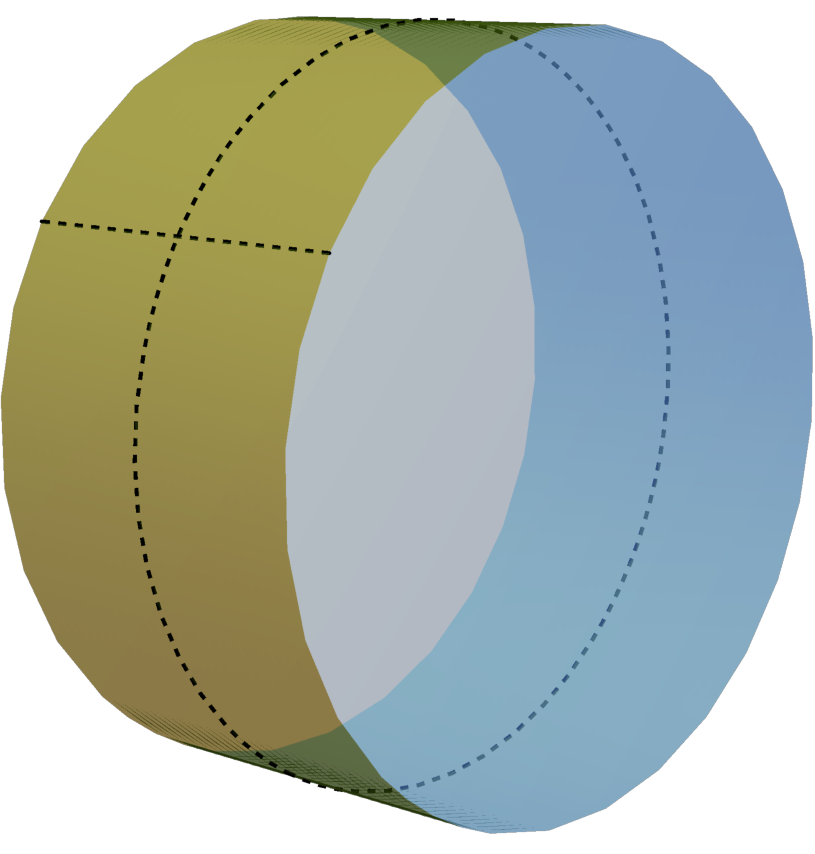
\includegraphics{Figures/Cilindro.pdf}
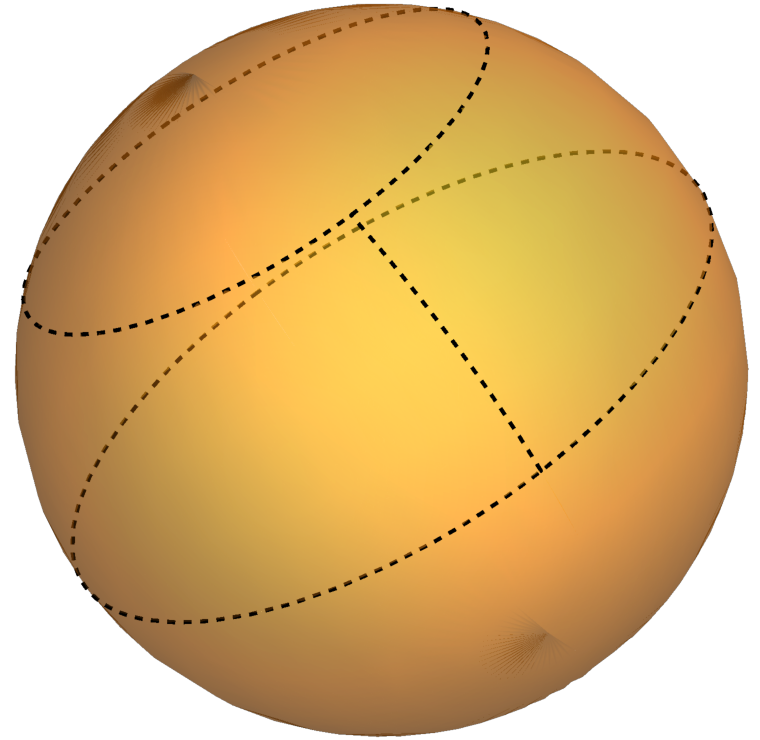
\includegraphics{Figures/Esfera.pdf}
\caption{Esfera y cilindro del \refexample{CilindroEsfera}. \labfig{Esfera}}
\end{marginfigure}

\begin{definition}
Sea $(X,A)$ un par de espacios. Tomando $C=S_*(X)$ y $D=S_*(A)$ en la
sucesión exacta (\ref{SECociente}), se obtiene la \textbf{sucesión exacta
asociada al par $(X,A)$}:
\[H_*(A) \xrightarrow{i_*} H_*(X) \xrightarrow{\pi_*} H_*(X,A)
\xrightarrow{\Delta} H_*(A)\]
\end{definition}

\begin{proposition}
$i_*$ es un isomorfismo si y sólo si $H_n(X,A)=0$ para todo $n \geq 0$.
\end{proposition}

Una \textbf{tríada de espacios} es una terna $(X,A,B)$, donde $(X,A)$ y
$(A,B)$ son pares de espacios.

Sea $(X,A,B)$ una tríada de espacios. Tomando $D=S_*(A)$, $E=S_*(B)$ y
$C=S_*(X)$ en \eqref{SECociente2}, se obtiene la sucesión exacta larga
\[H_n(A,B) \xrightarrow{i_*} H_n(X,B) \xrightarrow{j_*} H_n(X,A)
\xrightarrow{\Delta'} H_{n-1}(A,B)\]
donde $i_*$ y $j_*$ son los homomorfismos inducidos en homología por las
inclusiones $i\colon S_*(A) \hookrightarrow S_*(X)$ y $j\colon S_*(B)
\hookrightarrow S_*(A)$ y $\Delta'$ es la aplicación \eqref{DeltaCPrima}.

Recordemos que el grupo libre generado por el vacío es el grupo trivial, de
forma que $S_*(\emptyset)=0$. Esto nos permite establecer un isomorfismo
natural entre $S_*(X)$ y $S_*(X,\emptyset)$:
\begin{diag}
S_*(X) \arrow[r] & S_*(X,\emptyset)\\[-8mm]
c \arrow[r, maps to] & \overline c
\end{diag}
De la misma forma, se tiene que $S_*(X,A,\emptyset) \cong S_*(X,A)$ y
$S_*(X)\cong S_*(X,\emptyset,\emptyset)$.

\section{Aplicaciones entre pares}
\begin{definition}
Sean $(X,A)$ e $(Y,B)$ dos pares de espacios topológicos. Una
\textbf{aplicación de pares}
\[f\colon (X,A) \longrightarrow (Y,B)\]
es una aplicación continua $f\colon X \longrightarrow Y$ tal que $f(A)
\subseteq B$.
\end{definition}

Si $\phi\colon \sigma_p \to X$ es un símplice singular tal que
$\phi(\sigma_p) \subset A$ y $f\colon (X,A) \to (Y,B)$ es una
aplicación de pares, $(f\circ\phi)(\sigma_p) \subset B$, por lo que
$f_\#(\phi)$ es un $p$-símplice singular de $B$. Dado que la elección de
$\phi$ es arbitraria y los $p$-símplices singulares conforman una base de
$S_*(A)$,
\[f_\#(S_*(A)) \subseteq S_*(B)\]
por lo que $f$ induce una aplicación de cadenas
\begin{diag}
f_\#\colon S_*(X,A) \arrow[r] & S_*(Y,B)\\[-8mm]
\overline c \arrow[r, maps to] & \overline{f(c)}
\end{diag}
que induce a su vez un homomorfismo entre los grupos de homología relativa,
\begin{diag}
f_*\colon H_*(X,A) \arrow[r] & H_*(Y,B)\\[-8mm]
\left[\overline c\right] \arrow[r, maps to] & \left[\overline{f(c)}\right]
\end{diag}

Sean $f,g\colon (X,A) \to (Y,B)$ aplicaciones entre pares de espacios.
Decimos que $f$ es \textbf{homotópica} a $g$ si existe una aplicación entre
pares de espacios $F\colon (X\times I, A\times I) \to (Y,B)$ tal que
$F(x,0)=f(x)$ y $F(x,1)=g(x)$. Observar que $F$, al ser aplicación de pares,
se supone continua y verifica que $F(A\times I) \subset B$.

\begin{theorem}
Si $f,g\colon (X,A) \to (Y,B)$ son homotópicas como aplicaciones de pares,
\[f_*=g_*\colon H_*(X,A) \longrightarrow H_*(Y,B)\]
\end{theorem}

Tomando $A=\emptyset=B$, se obtiene el teorema de invarianza homotópica.

\begin{proof}
Sean $i_0,i_1\colon (X,A) \to (X\times I,A\times I)$ las aplicaciones
\begin{align*}
i_0(x)=(x,0); && i_1(x)=(x,1)
\end{align*}
Tenemos que $f=F\circ i_0$ y $g=F\circ i_1$. Para probar que $f_*=g_*$,
basta con probar que $(i_0)_\#$ e $(i_1)_\#$ son homotópicas como
aplicaciones de cadenas. La demostración es análoga al teorema de invarianza
homotópica.
\end{proof}

\begin{example}
Sean $X=[0,1]$, $Y=S_1 \subset \mb{R}^2$, $A=\{0,1\}$ y $B=\{(1,0)\}$.
Considérense las aplicaciones continuas $f,g\colon X \to Y$ definidas como
\begin{align*}
f(x)=e^{2\pi i x}; && g(x)=(1,0)
\end{align*}
Las aplicaciones $f$ y $g$ son homotópicas vía
\[F(x,t)=f(x)(1-t)+t\]
y además $f(A)=g(A)=B$, pero no forman una homotopía de pares entre $(X,A)$
e $(Y,B)$.
\end{example}

\subsection{Teorema de escisión}
\begin{lemma}[Lema de los cinco, \cite{FiveLemma}]
Sean $A_1,B_1,\dots,A_5,B_5$ grupos abelianos. Considérese el diagrama
conmutativo
\begin{diag}
A_1 \arrow{r} \arrow{d}{\alpha} & A_2 \arrow{r} \arrow{d}{\beta_1} &
A_3 \arrow{r} \arrow{d}{\gamma} & A_4 \arrow{r} \arrow{d}{\beta_2} &
A_5 \arrow{d}{\delta}\\
B_1 \arrow{r} & B_2 \arrow{r} & B_3 \arrow{r} & B_4 \arrow{r} & B_5
\end{diag}
cuyas filas forman sucesiones exactas. Si $\alpha$ es un epimorfismo,
$\beta_1$, $\beta_2$ son isomorfismos y $\delta$ es un monomorfismo,
$\gamma$ es un isomorfismo.
\end{lemma}

\begin{theorem}[Teorema de escisión]
Sea $(X,A)$ un par de espacios y $U \subset A$ tal que $\overline{U}
\subset \mathring A$. La aplicación inclusión $i\colon
(X\backslash U,A\backslash U) \hookrightarrow (X,A)$ induce un isomorfismo
\[i_*\colon H_*(X\backslash U,A\backslash U) \longrightarrow H_*(X,A)\]
\end{theorem}

\begin{marginfigure}
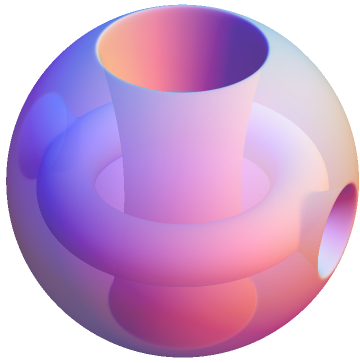
\includegraphics{Figures/HoleHoleHole.png}
\caption[Agujero en un agujero en un agujero]{El teorema de escisión nos dice
que la homología relativa de $X$ módulo $A$ sólo concierne a la frontera de
$A$. La estructura global del espacio no es relevante. Imagen: \cite{Hole}.}
\end{marginfigure}

\begin{proof}
Sea $\mc{U}=\{X\backslash U, \mathring A\}$. Tenemos por hipótesis que
\[(X\backslash U)^o=X\backslash\overline{U} \supset X\backslash\mathring{A}\]
por lo que $(X,\mc{U})$ es un espacio de Mayer-Vietoris. Si $\mc{U}'=
\{\mathring A,A\backslash U\}$, $(A,\mc{U}')$ también describe un espacio de
Mayer-Vietoris.

Los homomorfismos
\begin{align*}
i\colon S_*^\mc{U}(X) \hookrightarrow S_*(X);&&
i'\colon S_*^{\mc{U}'}(A) \hookrightarrow S_*(A)
\end{align*}
forman isomorfismos entre los grupos de homología. Teniendo en cuenta que
$S_*^{\mc{U}'}(A) \leq S_*^\mc{U}(X)$, la aplicación inclusión
\[j\colon S_*^{\mc{U},\mc{U}'}(X,A)=\frac{S_*^\mc{U}(X)}{S_*^{\mc{U}'}(A)}
\hookrightarrow \frac{S_*(X)}{S_*(A)}=S_*(X,A)\]
forma una aplicación de cadenas que da lugar al diagrama conmutativo
\begin{diag}
H_*(S_*^{\mc{U}'}(A)) \arrow{r} \arrow{d}{i'_*} &
H_*(S_*^\mc{U}) \arrow{r} \arrow{d}{i_*} &
H_*(S_*^{\mc{U},\mc{U}'}(X,A)) \arrow{r} \arrow{d}{j_*} &
H_*(S_*^{\mc{U}'}(A)) \arrow{d}{i_*}\\
H_*(A) \arrow{r} & H_*(X) \arrow{r} & H_*(X,A) \arrow{r} & H_*(A)
\end{diag}

\marginnote[-2.2cm]{
\begin{kaobox}[frametitle=Un detalle importante]
Dados tres grupos abelianos $A,B,C$ tales que $B+C \leq A+C$,
\[\frac{A+C}{B+C}\cong \frac{A}{B}\]
\end{kaobox}
}

Como $i_*$ e $i'_*$ son isomorfismos, el lema de los cinco nos garantiza que
$j_*$ es un isomorfismo, por lo que $S_*(X\backslash U,A\backslash U) \cong 
S_*^{\mc{U},\mc{U}'}(X,A)$ y concluimos que
\[H_*(X,A)\cong H_*(S_*^{\mc{U},\mc{U}'}(X,A)) \cong
H_*(X\backslash U,A\backslash U)\]
\end{proof}

\begin{example}\labexample{ToroAlambre}
\begin{enumerate}
\item Sea $X$ la esfera de la \reffig{Esfera}, $A$ el área
comprendida entre las dos circunferencias y $U\subset A$ una circunferencia
paralela a $\p A$. Tenemos que $X\backslash U$ son dos casquetes y
$A\backslash U$ son dos bandas. Ahora bien, observar que
\[\frac{X\backslash U}{A\backslash U} \cong \frac{X}{A}\]
por lo que ambos espacios tienen el mismo tipo de homología.
\item Sea $X$ el toro de Clifford,
\[A=\{[(x,y)] \in X\colon 1/4 \leq x \leq 3/4\}\]
y $\star \in A$. El subespacio $X\backslash\{\star\}$ es un toro
perforado. Podemos tomar el agujero y ensancharlo hasta quedarnos con dos
\emph{hilos de alambre} cruzados (que son los generadores de $H_1$). Esos
hilos forman una figura ocho.

Por otro lado, $A\backslash\{\star\}$ es un cilindro perforado. Podemos tomar
la perforación y ensancharla hasta quedarnos con las anillas de los bordes y
un alambre que los une. Dicho alambre se puede retraer hasta que las dos
anillas sean tangentes, formando una figura ocho.
\end{enumerate}
\end{example}

\begin{marginfigure}
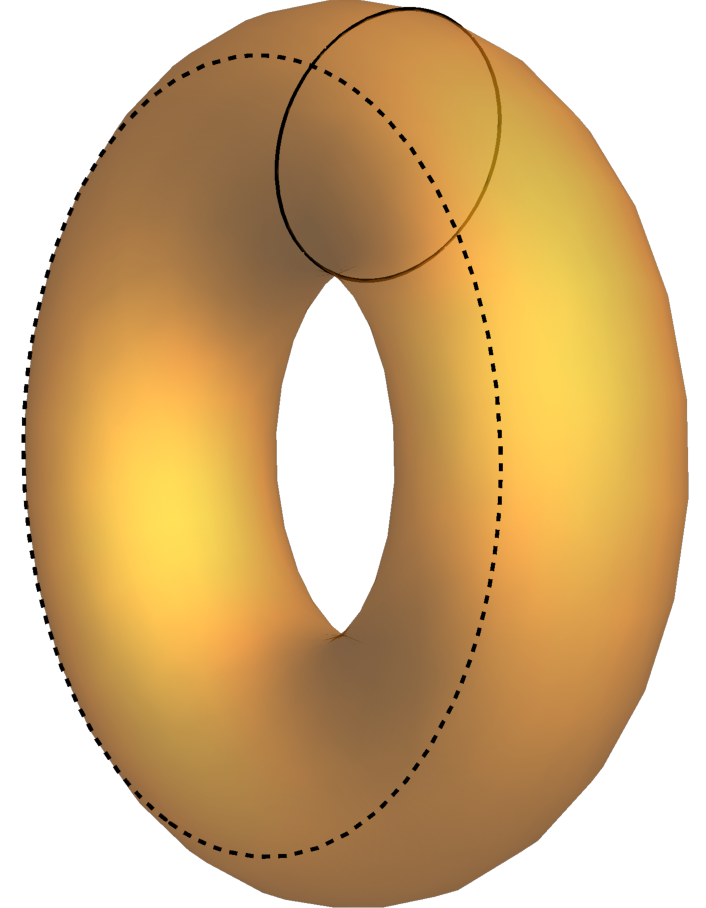
\includegraphics{Figures/ToroGeneradoresOrden1.pdf}
\caption{Generadores del grupo de homología de primer orden del toro.}
\end{marginfigure}

\section{Grupo de homología reducida}
Sea $X$ un espacio topológico. El camino constante
$\alpha\colon X \to \{\star\}$ da lugar a un homomorfismo en homologías
$\alpha_*\colon H_*(X) \to H_*(\{\star\})$. Se define el \textbf{grupo de
homología reducida} $\tilde H_*(X)$ como el núcleo de $\alpha_*$.

Si $X$ es convexo, sabemos por el \refthm{Convexo} que $H_n(X)=\{0\}$ para
todo $n > 0$, por lo que $\tilde H_n(X)=\{0\}$. Aún así, no podemos decir nada
del grupo de orden 0, porque $H_0(X)\cong \mb{Z}$.

La homología reducida está creada para poder describir de forma más sencilla
la homología de algunos espacios. Por ejemplo: todos los grupos de homología
reducida del espacio puntual son triviales, y el único grupo de homología
reducida no trivial de $S^n$ es el de orden $n$, como veremos más adelante.

En general, si un espacio es arcoconexo, su grupo de homología reducida de
orden cero es trivial.

\begin{proposition}
Sea $X$ un espacio topológico no vacío con una cantidad finita de
arcocomponentes. $\tilde{H}_0(X)$ es un grupo libre que verifica
\[\rk(\tilde{H}_0(X))=\rk(H_0(X))-1\]
\end{proposition}

\begin{proof}
Sea $c$ un $0$-ciclo de $X$. Si llamamos $X_1,\dots,X_n$ a las
arcocomponentes de $X$, existirán $a_1,\dots,a_n \in \mb{Z}$ tales que
\[c=\sum^n_{i=1}a_ix_i; \quad x_i \in X_i\]
Dado que $\alpha$ es una aplicación constante, podemos llamar $\alpha_0$ al
valor que toma en todos sus puntos, de forma que
\[0=\alpha_*([c])=\sum^n_{i=1}a_i[\alpha(x_i)]=[\alpha_0]\sum^n_{i=1}a_i\]

De aquí se deduce que $[c] \in \ker \alpha_*$ si y sólo si
\[a_n=-\sum^{n-1}_{i=1}a_i\]
por lo que $\{x_1,\dots,x_{n-1}\}$ forma un sistema generador libre de
$\tilde{H}_0(X)$. Por tanto,
\[\tilde{H}_0(X) \cong \mb{Z}^{n-1} \implies \rk(\tilde{H}_0(X))=
n-1=\mbox{rk }(H_0(X))-1\]
\end{proof}

Sea $f\colon X \to Y$ una aplicación continua. Al igual que $f$ induce un
homomorfismo entre grupos de homología, queremos ver que $f$ induce un
homomorfismo entre grupos de homología reducida. Para ello, sean $\alpha\colon
X \to \{\star\}$, $\beta\colon Y \to \{\star\}$ caminos constantes y $c=a_1x_1+
\dots+a_nx_n$ tal que $[c] \in \tilde H_n(X)$. Tenemos que
\[f_*([c])=\sum^n_{i=1}a_i[f(x_i)]=\sum^m_{j=1}b_j[y_j]\]
Dado que las aplicaciones continuas llevan conjuntos arcoconexos en conjuntos
arcoconexos,
\[\sum^n_{i=1}a_i=\sum^m_{j=1}b_j\]

Si $[c]$ está en $\ker \alpha_*$, la suma de todos los $a_i$ es 0. Como la
suma de los $a_i$ es la misma que la de los $b_j$, esto es tanto como decir
que $f_*([c])$ está en $\ker \beta_*$. Por tanto, $f_*(\ker \alpha_*) \leq
\ker \beta_*$, de forma que $f$ induce un homomorfismo entre los grupos de
homología reducida de $X$ e $Y$.

\begin{example}
Si $X$ es un espacio contráctil, $\tilde{H}_*(X)=0$.
\end{example}

\subsection{Una fórmula para la homología reducida}
\begin{lemma}[Lema de escisión]
Sean $A,B,C$ grupos abelianos. Considérese la sucesión exacta corta
\[0 \longrightarrow A \xrightarrow{f} B \xrightarrow{g} C \longrightarrow 0\]
Las siguientes afirmaciones son equivalentes:
\begin{enumerate}
\item $B$ es suma directa de $A$ con $C$;
\item existe un homomorfismo $h\colon B \to A$ tal que $f\circ h=\id_A$;
\item existe un homomorfismo $k\colon C \to B$ tal que $k\circ g=\id_C$.
\end{enumerate}
\end{lemma}

\begin{proposition}\labprop{ReducidoRelativo}
Dado un $p \in X$,
\[\tilde{H}_*(X)\cong H_*(X,\{p\})\]
\end{proposition}

\begin{proof}
Sea $i\colon \{p\} \hookrightarrow X$ la inclusión. La aplicación continua
\[\alpha: X \longrightarrow {p}\]
verifica que $\id_{\{p\}}=\alpha\circ i$, por lo que $\{p\}$ forma un
retracto de $X$ e $i_*$ es un monomorfismo.

Considérere la sucesión exacta de homología generada por el par de espacios
$(X,\{p\})$:
\[H_n(\{p\}) \xrightarrow{i_*} H_n(X) \xrightarrow{j_*}
H_n(X,\{p\}) \xrightarrow{\Delta'} H_{n-1}(\{p\})\]
Como $i_*$ es un monomorfismo, $\im \Delta'=\ker i_*=0$. Por el primer teorema
de isomorfia, $\im j_*=\ker \Delta'=H_n(X,p)$, por lo que $j_*$ es sobreyectiva.

Dado que $i_*$ es inyectiva y $j_*$ es sobreyectiva, podemos pasar a definir
una sucesión exacta corta en lugar de trabajar con una sucesión exacta
larga:
\[0 \longrightarrow H_n(\{p\}) \xrightarrow{i_*} H_n(X) \xrightarrow{j_*}
H_n(X,\{p\}) \longrightarrow 0\]

Sabemos que $\alpha_* \circ i_*=\id_{H_*(\{p\})}$, por lo que el lema de
escisión nos garantiza que existe un homomorfismo
\[\beta\colon H_n(X,\{p\}) \to H_n(X)\]
tal que $j_*\circ \beta=\id_{H_n(X,\{p\})}$. Esto es tanto como decir que
$\beta$ es inyectiva.

Se puede probar que $\im \beta=\ker \alpha_*=\tilde{H}_*(X)$, por lo que
hemos hallado un isomorfismo entre $H_*(X,\{p\})$ y $\tilde{H}_*(X)$.
\end{proof}

Sea $X$ un espacio topológico con $n$ componentes arcoconexas. Hasta ahora,
sabemos que
\[\tilde H_0(X) \cong \mb{Z}^{n-1}\]
pero queda pregunta preguntarnos qué ocurre con los grupos de orden
superior. Utilizando la \refprop{ReducidoRelativo}, tenemos para cada $p > 0$ y
el espacio puntual $\star$ que
\[\tilde{H}_p(X)\cong H_p(X,\star)=\frac{Z_p(X,\star)}{B_p(X,\star)}=
\frac{Z_p(X)/Z_p(\star)}{B_p(X)/B_p(\star)}\]
Teniendo en cuenta que $Z_p(\star)=B_p(\star)$, estamos en condiciones de
aplicar el tercer teorema de isomorfia:
\[\tilde{H}_p(X)\cong \frac{Z_p(X)/Z_p(\star)}{B_p(X)/B_p(\star)}=
\frac{Z_p(X)/B_p(\star)}{B_p(X)/B_p(\star)} \cong
\frac{Z_p(X)}{B_p(X)}=H_p(X)\]

De esta forma, llegamos a que el grupo de homología reducida sólo
\textit{reduce} el grupo de orden cero, cuya única función es contar el
número de componentes conexas.

\begin{corollary}\label{HomoReducida}
Sea $X$ un espacio topológico con una cantidad finita de arcocomponentes.
\[\tilde{H}_*(X)\cong \frac{H_*(X)}{H_*(\star)}\]
\end{corollary}

\begin{example}
$$\tilde{H}_*(B_p)\cong\frac{H_*(B_p)}{H_*(\star)}\cong
\begin{cases}\mb{Z}^p & \mbox{ si } n=1\\0 & \mbox{ si no}\end{cases}$$
\end{example}

\subsection{Homología reducida y homología relativa}
En lo sucesivo, diremos que un espacio topológico es de \textbf{tipo $C_2$}
si es compacto y $T_2$ al mismo tiempo.

\marginnote[-2.2cm]{
\begin{kaobox}[frametitle=Idea de la demostración]
En el lema, nos proporcionan una aplicación cociente $\pi$ que
envía $X$ en $X_A$ de forma continua, por lo que nuestro impulso inicial
sería definir
\[G=\pi \circ F \circ (\pi \times \id_I)^{-1}\]
El problema es que $\pi^{-1}$ no está bien definido, por lo que tampoco lo va
a estar $(\pi\times \id_I)^{-1}$. Lo que haremos será definir una $G$ tal que
\[G\circ \pi=(\pi\circ\id_I)\circ F\]
\end{kaobox}
}

\begin{lemma}\label{RetrCoci}
Sea $(X,A)$ un par de espacios donde $X$ es $C_2$ y $A$ es cerrado en $X$.
Considérese la aplicación cociente
\[\pi\colon X \to \frac{X}{A}\]
y sea $y=\pi(A) \in X/A$. Si $A$ es retracto por deformación fuerte de $X$,
$\{y\}$ es un retracto por deformación fuerte de $\pi(X)=X/A$.
\end{lemma}

\begin{proof}
Dado que $A$ es un retracto por deformación fuerte de $X$, existe una
homotopía $F\colon X \times I \to X$ tal que $F(x,0)=x$ para todo $x \in X$,
$F(a,t)=a$ para todo $a \in A$ y $t \in I$, y $F(X\times\{1\}) \subseteq A$.

Si $X_A=X/A$, queremos hallar una homotopía $G\colon X_A\times I \to X_A$ tal
que $G([x],0)=x$ para todo $x \in X_A$, $G(X_A\times\{1\})=\{y\}$ y $G(y,t)=y$
para todo $t \in I$.

Sea $G\colon X_A\times I \longrightarrow X_A$ la aplicación
\[G([x],t)=(\pi\circ F)(x,t)\]
Si $x \not\in A$, la clase de $x$ módulo $A$ es el singulete formado por el
propio punto $x$, por lo que $G$ está bien definido en $X_A\backslash\{y\}$.

Si $x \in A$, sabemos que $F(a,t)=a$ para todo $t \in I$, por lo que
\[(\pi\circ F)(a,t)=\pi(a) \in \pi(A)=\{y\}\]
De esta forma, $G$ está bien definida y que $G(y,t)=y$ para todo $t \in I$.

Sea $p \in X/A$. Si $x \in \pi^{-1}(p)$, sabemos que $F(x,0)=x$, por lo que
\begin{align*}
G(p,0)&=(\pi\circ F)(x,0)=\pi(x)=p\\
G(p,1)&=(\pi \circ F)(x,1)\in \pi(A)=\{y\}
\end{align*}

\marginnote[-2.2cm]{
\begin{kaobox}[frametitle=Detalles de la prueba]
\begin{itemize}
\item Una aplicación es continua si y sólo si la preimagen de todo cerrado es
cerrada.
\item Los subespacios cerrados de un compacto son compactos.
\item La imagen de un compacto por una aplicación continua es compacta.
\item Todo subespacio compacto de un espacio de Hausdorff es cerrado.
\end{itemize}
\end{kaobox}
}
Sólo nos queda ver que $G$ es continua. Para ello, sea $C$ un subconjunto
cerrado de $X/A$. Por continuidad, $D=(\pi\circ F)^{-1}(C)$ es un subconjunto
cerrado de $X\times I$. Como $X\times I$ es compacto, $D$ es compacto. Por
continuidad, $(\pi\times \id_I)(D)$ es compacto. Por cómo se define $G$,
\[G^{-1}(C)=(\pi\times 1_I)(D) \subseteq X_A \times I\]
es compacto. Dado que
$X_A\times I$ es un espacio de Hausdorff, $G^{-1}(C)$ es cerrado.

Dado que la elección de $C$ es arbitraria, se sigue que $G$ es continua.
\end{proof}

\begin{lemma}
Sea $X$ un espacio $C_2$. Dados dos cerrados disjuntos $C,D \subset X$,
existen abiertos $U,V \subset X$ tales que $U$ contiene a $C$, $V$ contiene
a $D$ y $U\cap V=\emptyset$
\end{lemma}

\begin{proof}
Dados $x \in C$ e $y \in D$, como $C$ y $D$ son disjuntos, $x \neq y$. Como
$X$ es un espacio de Hausdorff, existen $U_y$, $V_y$ abiertos tales que
\begin{align*}
x \in U_y; && y \in V_y; && U_y\cap V_y=\emptyset
\end{align*}
Como $D$ es un subespacio cerrado de un compacto, $D$ es compacto, por lo
que podemos hallar una familia finita de puntos $y_1,\dots,y_n \in D$ tales
que $\{V_{y_1},\dots, V_{y_n}\}$ forma un recubrimiento abierto de $D$.

Para cada $i \in \{1,\dots,n\}$, podemos hallar un abierto $U_i \subseteq X$
tal que $U_i\cap V_{y_i}=\emptyset$ y $x \in U_i$. Se  definen entonces
\begin{align*}
U_x=\bigcup_{i=1}^nU_i;&&  V_x=\bigcup_{i=1}^n V_{y_i}
\end{align*}
Notar que ambos conjuntos son abiertos y $U_x\cap V_x=\emptyset$.

Dado que $C$ es un subespacio cerrado de un compacto, $C$ es compacto, por
lo que podemos hallar una familia finita de puntos $x_1,\dots,x_n$ tales que
$\{U_{x_1},\dots,U_{x_m}\}$ forma un recubrimiento abierto de $C$.

Para terminar, considérense los abiertos
\begin{align*}
U=\bigcup _{i=1}^m U_{x_i};&&  V=\bigcup_{i=1}^m V_{x_i}
\end{align*}
Se tiene por construcción que $D \subseteq V$ y $U\cap V=\emptyset$.
\end{proof}

\begin{lemma}\lablemma{LemaB}
Sea $X$ un espacio $C_2$. Dado un cerrado $A$ contenido en un abierto $V$,
existe un abierto $W$ tal que
$$A \subseteq W \subseteq \overline{W} \subseteq V$$
\end{lemma}

\begin{proof}
Considérense los cerrados $A$ y $X\backslash V$. Por el lema anterior, existen
abiertos $U,W$ de $X$ tales que $A \subseteq W$, $X\backslash V \subseteq U$ y
$U\cap W=\emptyset$. Tenemos que $U\cap W=\emptyset$, por lo que
\[W \subseteq X\backslash U \subseteq V \implies
\overline{W} \subset \overline{X\backslash U}=X\backslash U \subseteq V\]
\end{proof}

\begin{theorem}[Teorema del retracto]\labthm{Retracto}
Sea $X$ un espacio $C_2$, $A$ un subespacio cerrado de $X$ y $\pi\colon (X,A)
\to (X/A,\pi(A))$ una aplicación cociente. Si $A$ es un retracto por
deformación fuerte de algún entorno cerrado de $A$ en $X$,
\[H_*(X,A) \cong H_*(X/A,\pi(A)) \cong \tilde{H}_*(X/A)\]
\end{theorem}

\begin{proof}
Considérese la sucesión exacta asociada a la tríada de espacios $(X,U,A)$:
\[H_*(U,A) \xrightarrow{i_*} H_*(X,A) \xrightarrow{j_*} H_*(X,U)
\xrightarrow{\Delta'} H_*(U,A)\]
Dado que $A$ es un retracto por deformación fuerte de $U$, $H_*(U,A)=0$. Por
exactitud, se sigue que $0=\im i_*=\ker j_*$ y $\im j_*=\ker \Delta'=
H_*(X,U)$. Por tanto,
\[H_*(X,A) \cong H_*(X,U)\]

Sabemos que $X$ es un espacio $C_2$ y que $A$ es cerrado. Como $U$ es
entorno de $A$, $A \subseteq \mathring U$. Usando el \reflemma{LemaB}, podemos
hallar un abierto $V \subseteq X$ tal que $A \subseteq V \subseteq
\overline{V} \subseteq \mathring U \subseteq U$. Aplicando el teorema de
escisión, la inclusión $i\colon (X\backslash V,U\backslash V) \hookrightarrow
(X,U)$ induce un isomorfismo $i_*$. Se sigue que
\[H_*(X,U)\cong H_*(X\backslash V,U\backslash V)\]

Considérese la aplicación $p=\pi|_{X\backslash V}$. Como $A \subseteq V$,
$\pi(x)$ sólo tiene un representante (el propio $x$), de forma que $p$ es un
homeomorfismo. Como $\pi(U\backslash V)=\pi(U)\backslash \pi(V)$, se sigue que
\[H_*(X\backslash V,U\backslash V)\cong
H_*(X_A\backslash \pi(V),\pi(U)\backslash \pi(V))\]

Aplicando el teorema de escisión al par $(X_A,\pi(U))$, se obtiene el
isomorfismo
\[H_*(X_A\backslash \pi(V),\pi(U)\backslash \pi(V)) \cong H_*(X_A,\pi(U))\]

Considérese la sucesión exacta asociada a la tríada de espacios\\
$(X_A,\pi(U),\pi(A))$. Un procedimiento similar al que hemos desarrollado al
inicio de la demostración nos lleva a concluir que
\[H_*(X_A,\pi(U))\cong H_*(X_A,\pi(A))\]
\end{proof}

\section{Homeomorfismo relativo}
\begin{definition}
Un \textbf{homeomorfismo relativo} es una aplicación continua entre pares de
espacios $f\colon (X,A) \to (Y,B)$ tal que
\[f\colon X\backslash A \longrightarrow Y\backslash B\]
es un homeomorfismo.
\end{definition}

\begin{example}
\begin{enumerate}
\item Si $\mc{N}=(0,0,1) \in S^2$ y $D^2$ denota a la bola cerrada unidad de
$\mb{R}^2$, existe un homeomorfismo
\[f\colon D^2\backslash \partial D^2 \longrightarrow S^2\backslash\{\mc{N}\}\]
De esta forma, $f$ induce un homeomorfismo relativo entre los pares 
$(S^2,\{\mc{N}\})$ y $(D^2,\partial D^2)$.
\item Si $C=S^1\times I$ es un cilindro y $\mc{S}=(0,0,-1) \in S^2$, existe un
homeomorfismo
\[g\colon S^1\times \mathring{I} \to S^2-\{\mc{N},\mc{S}\}\]
que identifica al cilindro sin anillas con $S^2$
\end{enumerate}
\end{example}

\begin{theorem}[Teorema del homeomorfismo relativo]\labthm{HomeoRelativo}
Sean $X$, $Y$ espacios $C_2$, $A \subseteq X$ y $B \subseteq Y$ cerrados y
$f\colon (X,A) \to (Y,B)$ un homeomorfismo relativo. Si $A$ es retracto por
deformación fuerte de algún entorno compacto de $A$ en $X$ y $B$ es retracto
por deformación fuerte de algún entorno compacto de $B$  en $Y$, $f_*$ es un
isomorfismo.
\end{theorem}

\begin{proof}
Sean $\pi\colon X \to X/A$ y $\pi'\colon Y \to Y/B$ aplicaciones cociente. Se
define la aplicación $f'\colon X/A \to Y/B$ como $f([x])=\pi'(f(x))$.
Es fácil ver que $f'$ está bien definida y es continua, por lo que da lugar
al siguiente diagrama conmutativo:
\begin{diag}
X \arrow{r}{f} \arrow{d}{\pi} & Y \arrow{d}{\pi'}\\
X/A \arrow{r}{f'} & Y/B
\end{diag}

Dado que $f$ es un homeomorfismo relativo, $f'$ es una biyección entre $X/A$
e $Y/B$. Como ambos son espacios $C_2$, $f'$ es un homeomorfismo, por lo que
induce un isomorfismo entre $H_*(X/A)$ y $H_*(Y/B)$.

Tenemos entonces el diagrama conmutativo
\begin{diag}
H_*(X,A) \arrow{r}{f_*} \arrow{d}{\pi_*} & H_*(Y,B) \arrow{d}{\pi'_*}\\
H_*(X/A,\pi(A)) \arrow{r}{f'_*} & H_*(Y/B,\pi'(B))
\end{diag}

Sabemos por el \refthm{Retracto} que $\pi'_*$ y $\pi_*$ son isomorfismos;
además, acabamos de probar que $f_*'$ es un isomorfismo. Como consecuencia,
$f_*$ es un isomorfismo.
\end{proof}

\setchapterpreamble[u]{\margintoc}

\chapter{Espacios CW-complejos} \label{CW}
\section{Espacio de adjunción}
\begin{definition}
Sean $X,Y$ espacios topológicos, $A \subset X$ un subespacio cerrado y
$f\colon A \to Y$ una aplicación continua. Dados $x \in X$, $y \in Y$,
escribiremos $x \sim y$ si $x \in A$ e $y=f(x)$. Se define el
\textbf{espacio de adjunción} o \textbf{de pegamiento} como
\[X \cup_f Y:=\frac{X\sqcup Y}{\sim}\]
Decimos que $f$ es la \textbf{aplicación de adjunción} o de
\textbf{pegamiento} de $X\cup_fY$.
\end{definition}

Si $Y=\{\star\}$, $f=\text{Cte}_\star$, por lo que $x\sim z$ para todos $x,z
\in A$ y $X\cup_f Y=X/A$.

\begin{lemma}
La proyección canónica $p\colon X \sqcup Y \to X\cup_f Y$ verifica las
siguientes condiciones:
\begin{enumerate}
\item $p(Y)$ es cerrado;
\item $p|_Y$ es un homeomorfismo sobre su imagen;
\item $p(X\backslash A)$ es abierto;
\item $p|_{X\backslash A}$ es un homeomorfismo sobre su imagen.
\end{enumerate}
Como consecuencia, podemos considerar a $Y$ y $X\backslash A$ como subespacios
de $X\cup_f Y$.
\end{lemma}

\marginnote[-2.2cm]{
\begin{kaobox}[frametitle=Aplicaciones abiertas y cerradas]
Una aplicación $f\colon X \to Y$ es abierta (resp. cerrada) si la imagen de
un abierto (resp. cerrado) en $X$ es abierto (resp. cerrado) en $Y$. Si $f$ es
biyectiva, su inversa será continua si y sólo si $f$ es abierta o cerrada.

Un ejemplo de aplicación abierta (y cerrada) son las proyecciones.
\end{kaobox}
}

\begin{proof}
Como $X\sqcup Y$ es una unión disjunta de espacios topológicos, $Y$ es un
subespacio cerrado de $X\sqcup Y$. Además, $A$ es cerrado en $X$ si y sólo si
lo es en $X \sqcup Y$, por lo que $A\cup Y$ es cerrado en $X \sqcup Y$. Pero
$A\cup Y=p^{-1}[p(Y)]$, por lo que $p(Y)$ es cerrado.

Pasemos al segundo ítem: para ver que $p|_Y$ es un homeomorfismo sobre su
imagen, necesitamos ver que es cerrada e inyectiva.

Sea $y\in Y$: si $y \not\in f(A)$, se tiene de forma trivial que $p^{-1}([y])=
\{y\}$. Si $y \in f(A)$, podemos hallar un $x \in A$ tal que $f(x)=y$.

Como $x \in A \subseteq X$, podemos hallar un $y' \in X\sqcup Y$ tal que $y
\sim y'$. Si $y' \in Y$, $y=f(x)=y'$ y no hay nada que probar. Si asumimos que
$y'\neq y$, $y \in X$. Teniendo en cuenta que 
\[(p|_Y)^{-1}([y])=p^{-1}([y])\cap Y\]
se sigue que $y' \not \in (p|_Y)^{-1}([y])$, por lo que $p|_Y$ es inyectiva.

Para ver que $p|_Y$ es cerrada, sea $C$ un subespacio cerrado de $Y$. Como
$p(Y)$ es cerrado en $X \cup_f Y$, $p(C)$ es cerrado en $p(Y)$ si y sólo si lo
es en $X \cup_f Y$. Ésto es tanto como decir que $p^{-1}[p(C)]$ es cerrado en
$X \sqcup Y$.

Observamos que
\[p^{-1}[p(C)]=f^{-1}(C)\sqcup C\]
por lo que $p^{-1}[p(C)]$ es una unión de cerrados. En consecuencia, $p(C)$ es
cerrado en $p(Y)$, de donde se sigue que $p|_Y$ es una aplicación cerrada.
Ésto concluye el segundo ítem.

Como $A$ es cerrado en $X$, $X\backslash A$ es abierto en $X \sqcup Y$. Dado
que\\ $p^{-1}[p(X\backslash A)]=X\backslash A$, se sigue que
$p(X\backslash A)$ es abierto en $X\cup_f Y$.

Pasemos al último item: dado un $x \in X\backslash A$, $p^{-1}([x])=\{x\}$,
por lo que $p|_{X\backslash A}$ es inyectivo. Dado que $p$ es continua, sólo
necesitamos ver que es abierta para deducir la tesis.

Sea $U\subseteq X\backslash A$: como $p(X\backslash A)$ es abierto en
$X\cup_f Y$, $p(U)$ será abierto en $p(X\backslash A)$ si y sólo si lo es en
el espacio de adjunción, o equivalentemente, $p^{-1}[p(U)]$ es abierto en
$X\sqcup Y$.

Dado que $U\subseteq X\backslash A$, se tiene que $U=p^{-1}[p(U)]$. Si $U$
es abierto de $X\backslash A$ también lo será de $X\sqcup Y$, por lo que
$p(U)$ es abierto en el espacio de adjunción. Ésto concluye la demostración.
\end{proof}

\marginnote[-2.2cm]{
\begin{kaobox}[frametitle=Primer axioma de numerabilidad]
Un espacio topológico $X$ verifica el primer axioma de numerabilidad (1AN)
si, dado $p \in X$, existe una base de entornos numberable de $X$.

Una base de entornos de $p$ es una familia de entornos $\{V_\alpha\colon
\alpha \in A\}$ tal que, dado un entorno $U \subseteq X$ de $p$, $U$
contiene al menos a un $V_\alpha$.
\end{kaobox}
}

\begin{lemma}
\label{AdjC2} Sean $X$, $Y$ espacios de tipo $C_2$. Si $X$ e $Y$ son 1AN,
$X\cup_f Y$ es de tipo $C_2$.
\end{lemma}

\begin{proof}
El espacio $X\cup_f Y$ es compacto por ser imagen de un espacio compacto
(en este caso $X\sqcup Y$) por una aplicación continua (la proyección
canónica $p\colon X\sqcup Y \to X\cup_f Y$).

Queremos ver que $X\cup_f Y$ es $T_2$. Dado que $X\cup_f Y$ es un espacio
cociente y $X$, $Y$ son $T_2$, basta ver que el conjunto
\[\{(x,y) \in (X\cup_f Y)^2\colon y=f(x)\}=G(f)\]
es cerrado. Dado que $X$ e $Y$ son 1AN, $(X\sqcup Y)^2$ es 1AN, por lo que
$G(f)$ será cerrado si y sólo si contiene a todos sus puntos de acumulación.

\marginnote[-2.2cm]{
\begin{kaobox}[frametitle=La propiedad de Hausdorff en los cocientes]
Sea $W$ un espacio de Hausdorff y $\sim$ una relación de equivalencia sobre
los puntos de $W$. Si el conjunto
\[\{(x,y) \in W^2: x\sim y\}\]
es cerrado en $W^2$, $W/\sim$ es un espacio de Hausdorff.
\end{kaobox}
}

Sea $(z_n)$ una sucesión de $G(f)$. Por compacidad de $X \sqcup Y$, existe
una subsucesión $(z_{n_k})$ convergente a un cierto $z_0 \in X\sqcup Y$. Por
definición de $G(f)$, existe una sucesión $(x_k)$ de $A$ tal que
\[z_{n_k}=(x_k,f(x_k))\]
Se tiene entonces que $(x_k)$ converge a $x_0$, que está en $A$ por ser
cerrado de $X$. Además, como $f$ es continua, $f(x_k)$ converge a $f(x_0)$.

De esta forma, $(z_{n_k})$ converge a $(x_0,f(x_0)) \in G(f)$. Dado que
$X\sqcup Y$ es $T_2$, $z_0=(x_0,f(x_0))$, por lo que $z_0 \in G(f)$. De aquí
se sigue que $G(f)$ es cerrado. Por tanto, $X\cup_f Y$ es $T_2$.
\end{proof}

\begin{lemma}\lablemma{RepAdj}
Sean $X$, $Y$, $W$ espacios $C_2$, $A \subset X$ un subconjunto cerrado y
$g\colon X\sqcup Y \to W$ una aplicación continua y sobreyectiva. Supongamos
que, para todo punto $w \in W$, se cumple que
\[g^{-1}(w)=\left\{
\begin{array}{c}
\text{un único punto de $X\backslash A$}\\
\lor\\
\text{$\{y\}\cup f^{-1}(y)$ para algún $y \in Y$}
\end{array}
\right.\]
Entonces, $g$ induce un homeomorfismo entre $W$ y $X \cup_f Y$.
\end{lemma}

\begin{proof}
Sea $\p\colon X\sqcup Y \to X \cup_f Y$ la proyección canónica. Se define la
aplicación
\begin{diag}
\overline g\colon X\cup_f Y \arrow[r]& W\\[-8mm]
\left[x\right] \arrow[maps to, r] & g(x)
\end{diag}

\marginnote[-2.2cm]{
\begin{kaobox}[frametitle=Continuidad de la inversa]
Si $f\colon X \longrightarrow Y$ es una biyección continua, donde $X$ es
compacto e $Y$ es de Hausdorff, $f$ es un homeomorfismo.
\end{kaobox}
}

Supongamos que $\overline g$ está bien definida y es una biyección continua:
por el \reflemma{AdjC2}, tenemos que $X\cup_f Y$ es de tipo $C_2$. Como $W$ es
$T_2$, se sigue que $\overline g$ tiene inversa continua, por lo que es un
homeomorfismo y el lema queda probado.

Empecemos por ver que $\overline{g}$ está bien definida: sean $x_1, x_2 \in
A$ elementos asociados y diferentes. Existirá un $y \in f(A)$ tal que $f(x_1)=
y=f(x_2)$. Si $w=g(x_1)$, se tiene por hipótesis que
\[g^{-1}(w)=\{y\}\cup f^{-1}(y) \implies g(x_1)=w=g(x_2)\]
Si $x \in X\backslash A$, $x$ sólo está asociado consigo mismo, de forma que
$\overline{g}$ está trivialmente bien definida. Dado que todas las
antiimágenes por $g$ de un cierto $w \in W$ están asociadas, $\overline{g}$ es
también inyectiva.

Veamos que $\overline{g}$ es continua: si $C \subseteq W$ es cerrado,
$g^{-1}(C)$ es cerrado en $X\sqcup Y$, por lo que $\pi^{-1}[g^{-1}(C)]$ es
cerrado en $X\cup_f Y$. Notar que
\[\pi^{-1}[g^{-1}(C)]=\overline{g}^{-1}(C)\]
por lo que se sigue la continuidad de $\overline{g}$.
\end{proof}

Sea $g\colon X \to W$ una aplicación continua y sobreyectiva entre espacios de
tipo $C_2$. Supongamos que existe un $w_0 \in W$ de forma que $A=g^{-1}(w_0)$
es un cerrado en $X$ y $g^{-1}(w)$ es un único punto de $X\backslash A$ para
todo $w\neq w_0$.

Si $\{\star\}$ es el espacio puntual, la aplicación constante
$f\colon A \to \{\star\}$ es continua, y se verifica que $X \cup_f \{\star\}$
es homeomorfo a $X/A$. Por el \reflemma{RepAdj}, se tiene que
\[W \cong X \cup_f \{\star\}\cong X/A\]

%Un espacio topológico Hausdorff y 2AN $X$ es una $n$-variedad si, dado $p \in
%$X$, existe un entorno abierto $U \subseteq X$ de $p$ homeomorfo a una bola
%abierta de $\mb{R}^n$. Éstos homeomorfismos se denominan cartas o
%parametrizaciones locales de $X$.

\begin{example} \label{Sn_CW}
Sea $h\colon D^n\backslash S^{n-1} \to \mb{R}^n$ un homeomorfismo, $\mc{N}=
(0,0,\dots,0,1)$ y $S^n_+=S^n\backslash\mc{N}$. La \textbf{proyección
estereográfica}, dada por
\begin{diag}
\Phi\colon S^n_+ \arrow[r] & \mb{R}^n\\[-8mm]
(x_1,\dots,x_{n+1}) \arrow[maps to, r] &
	\displaystyle\left(\frac{x_1}{1-x_{n+1}},\dots,\frac{x_n}{1-x_{n+1}}\right)
\end{diag}
es un homeomorfismo. Una posible parametrización de $h$ es
\[h(z)=\frac{z}{1-\|z\|}\]
Se define la aplicación $g\colon D^n \to S^n$ dada por
\[g(x)=\begin{cases}
\mc{N} &\text{ si $x \in S^{n-1}$}\\
(\Phi^{-1}\circ h)(x) &\text{ si $x \in D^n\backslash S^{n-1}$}
\end{cases}\]
Se tiene entonces que $g$ es continua y sobreyectiva por construcción.

Como $\mc{N} \in S^{n-1}$, $g^{-1}(\mc{N})=\{\mc{N}\}$ es un cerrado en $D^n$.
Dado que $\Phi$ y $h$ son aplicaciones biyectivas, $g^{-1}(z)$ es un único
punto para todo $z\neq \mc{N}$. Aplicando el lema \reflemma{RepAdj}, se tiene
entonces que
\[S^n\cong \frac{D^n}{S^{n-1}}\]
que es la adjunción de $D^n$ a un espacio puntual.
\end{example}

\begin{marginfigure}
\resizebox{\textwidth}{!}{
\begin{tikzpicture}
\draw[fill=blue] (0,0) circle (1pt);

\draw[dashed, -to] (.8,.8) -- (.2,.2);
\draw[dashed, -to] (.8,-.8) -- (.2,-.2);

\draw[fill=blue] (1,1) circle (1pt) -- (1,-1) circle (1pt);

\draw[|-stealth] (1.5,0) -- (2,0);

\draw (3.5,0) node {$S^1$} circle (1cm);
\draw[fill=blue] (2.5,0) circle (1pt);
\end{tikzpicture}
}
\caption{\labfig{CWS1} Conjunto $S^1$ construido como espacio de adjunción.}
\end{marginfigure}
\begin{marginfigure}
\resizebox{\textwidth}{!}{
\begin{tikzpicture}
\draw (3.5,0) circle (1cm);
\draw[fill=blue] (2.5,0) circle (1pt);

\draw (3.5,-1) .. controls (2,-1) and (1.5,0) .. (0,0);
\draw (3.5,1) .. controls (2,2) and (1.5,0) .. (0,0);
\end{tikzpicture}
}
\caption[Espacio $S^1$ con dos segmentos adicionales, creando una figura
ocho.]{Podemos adjuntar nuevas células a las células preexistentes para
recrear espacios más complejos.}
\end{marginfigure}


\subsection{Células y adjunción}
Supongamos que $X=D^n$ para algún $n > 0$ y $A=S^{n-1}=\p D^n$. Decimos que el
espacio
\[Y_f:=D^n\cup_f Y\]
es la \textbf{adjunción de una $n$-célula} al espacio $Y$.

\begin{example}\labexample{Sn_CW}
En la figura \reffig{CWS1}, vemos cómo $S^1\cong \{\star\}_f$, siendo
$f\colon \p D^1=\{0,1\}\to \{\star\}$ la aplicación constante. En general,
$S^n$ se puede obtener como $\{\star\}_{f_n}$, siendo $f_n\colon \p D^n \to
\{\star\}$.
\end{example}

\begin{lemma}\lablemma{EntornoCompacto}
Sea $f: S^{n-1} \to Y$ una aplicación continua. Si $Y$ es un espacio $C_2$,
existe un entorno compacto $U_f$ de $Y$ en $Y_f$ tal que $Y$ es un retracto
por deformación fuerte de $U_f$.
\end{lemma}

\begin{proof}
Sea $U=\{x \in D^n: \|x\| \geq 1/2\}$. El cerrado $U$ es un entorno compacto
de $S^{n-1}$ en $D^n$. Definimos la homotopía $F\colon (U \sqcup Y)\times I
\to U\sqcup Y$ como
\[F(x,t)=
\begin{cases}
x &\text{ si }x \in Y \\
\displaystyle
(1-t)x+t\frac{x}{\|x\|} &\text{ si }x \in U
\end{cases}\]

Tenemos que $F$ es una aplicación continua que verifica las siguientes
propiedades:
\begin{enumerate}
\item $F(x,0)=x$ para todo $x \in U\sqcup Y$.
\item $F(x,1) \in S^{n-1}\sqcup Y$ para todo $x \in U \sqcup Y$.
\item $F(x,t)=x$ para todo $x \in S^{n-1}\sqcup Y$ y todo $t \in I$.
\end{enumerate}
Se sigue que $S^{n-1}\sqcup Y$ es un retracto por deformación fuerte de
$U\sqcup Y$.

Si $p\colon D^n \sqcup Y \to Y_f$ denota a la proyección canónica, se define
$U_f$ como la imagen de $U$ mediante $p$. Queremos ver que $Y$ es un retracto
por deformación fuerte de $U_f$ en $Y_f$. Para ello, considérese la
homotopía
\begin{diag}
G\colon U_f\times I \arrow[r] & U_f\\[-8mm]
(\left[x\right],t)\arrow[maps to,r] & F(x,t)
\end{diag}

Es fácil ver que $G$ está bien definida. Para ver que es continua, considérese
el diagrama conmutativo
\begin{diag}
(U\sqcup Y)\times I \arrow{r}{F} \arrow{d}{p\times \id_I}&
	U\sqcup Y \arrow{d}{p}\\
U_f\times I \arrow{r}{G} & U_f
\end{diag}

Dado que $F$ y $p$ son continuas, $G\times (p\times \id_I)=p\circ F$ es
continua, por lo que $G$ es continua. De aquí se sigue que $Y$ es un retracto
por deformación fuerte de $U_f$.
\end{proof}

\begin{proposition}
Dada una aplicación continua $f\colon S^{n-1} \to Y$,
\[H_p(Y_f,Y)\cong
\begin{cases}
\mb{Z} & \text{ si $p=n$}\\
0 & \text{ si no}
\end{cases}\]
\end{proposition}

\begin{proof}
Consideremos la composición
\[h\colon D^n \hookrightarrow D^n\sqcup Y \xrightarrow{p} Y_f\] 
El espacio $D^n\backslash S^{n-1}$ es homeomorfo a $Y_f\backslash Y$, puesto
que $Y_f=Y\cup_f D^n$, de forma que $h$ induce un homeomorfismo relativo entre
los pares $(D^n,S^{n-1})$ e $(Y_f,Y)$.

La esfera $S^{n-1}$ es un retracto por deformación fuerte del entorno compacto
$U=\{x \in D^n: \|x\| \geq 1/2\}$, y sabemos por el
\reflemma{EntornoCompacto} que $Y$ es un retracto por deformación fuerte de
algún entorno $U_f$ compacto de $Y$ en $Y_f$. Por el teorema del homeomorfismo
relativo (\refthm{HomeoRelativo}), se tiene que
\[h_*\colon H_*(D^n,S^{n-1}) \longrightarrow H_*(Y_f,Y)\]
es un isomorfismo.

Se tiene entonces que
\[H_*(Y_f,Y) \cong H_*(D^n,S^{n-1}) \cong \tilde{H}_*(S^n)\cong
\begin{cases}
\mb{Z} & \text{ si }p=n \\
0 & \text{ si no}
\end{cases}\]
\end{proof}

\begin{proposition} \labprop{HomoCW}
Sea $Y$ un espacio topológico y $f\colon S^{n-1} \to Y$ una aplicación
continua. Si $f_*\colon \tilde{H}_{n-1}(S^{n-1}) \to H_{n-1}(Y)$,
\begin{enumerate}
\item $H_p(Y_f)\cong H_p(Y)$ para todo $p$ distinto a $n$ y $n-1$;
\item $H_{n-1}(Y_f)\cong H_{n-1}(Y)/\im f_*$;
\item la sucesión
\begin{diag}
0 \arrow[r]& H_n(Y) \arrow[r]& H_n(Y_f) \arrow[r]&
\ker f_* \arrow[r]& 0
\end{diag}
es exacta.
\end{enumerate}
\end{proposition}

\begin{proof}
Consideremos la sucesión exacta larga asociada al par de espacios $(Y_f,Y)$:
\[\dots \longrightarrow H_{p+1}(Y_f,Y) \longrightarrow H_p(Y)
\xrightarrow{\beta} H_p(Y_f) \longrightarrow H_p(Y_f,Y) \longrightarrow \dots\]
Como vimos en el \refexample{Sn_CW},
\[H_p(Y_f,Y)\cong \tilde{H}_p(S^n) \cong \tilde{H}_{p-1}(S^{n-1})\]

Para $p\neq n,n-1$, $\tilde{H}_p(S^n)=0$, por lo que $\ker
\beta=0$ y $\im \beta=H_p(Y_f)$. Se sigue entonces la primera afirmación:
\[H_p(Y_f) \cong H_p(Y)\]

Para $p=n$ y $p=n-1$, se tiene la sucesión exacta
\begin{align*}
0=\tilde{H}_n(S^{n-1}) &\longrightarrow H_n(Y) \longrightarrow H_n(Y_f)
\xrightarrow{\beta} \tilde{H}_{n-1}(S^{n-1}) \xrightarrow{f_*} \\
&\xrightarrow{f_*} H_{n-1}(Y) \xrightarrow{\alpha} H_{n-1}(Y_f)
\longrightarrow \tilde{H}_{n-2}(S^{n-1})=0
\end{align*}
donde $\im \beta=\ker f_*$, $\im f_*=\ker \alpha$ y $\im \alpha=H_{n-1}(Y_f)$
por exactitud. Aplicando el primer teorema de isomorfia, se tiene la segunda
afirmación:
\[H_{n-1}(Y_f)=\im \alpha \cong \frac{H_{n-1}(Y)}{\ker \alpha}=
\frac{H_{n-1}(Y)}{\im f_*}\]

Ahora bien: como $\im \beta=\ker f_*$, la sucesión
\[0 \longrightarrow H_n(Y) \longrightarrow H_n(Y_f) \xrightarrow{\beta}
\ker f_* \longrightarrow 0\] es exacta, que es la tercera afirmación.
\end{proof}

\section{Espacios CW-complejos}
Sean $D_1^n,\dots, D_p^n$ una familia de $n$-células disjuntas con respectivas
fronteras $S^{n-1}_1,\dots,S^{n-1}_p$. Dado un $1 \leq i \leq p$, considérese
la aplicación continua
\[f_i\colon S^{n-1}_i \longrightarrow Y\]
siendo $Y$ un espacio topológico arbitrario. Si $\mc{D}^n=D^n_1\sqcup\dots
\sqcup D^n_p$ y $\mc{S}^{n-1}=\p \mc{D}^n=S^{n-1}_1\sqcup \dots S^{n-1}_p$,
definimos sobre $\mc{D}^n\sqcup Y$ la siguiente relación de equivalencia:
\[\forall x \in S^{n-1}_i \quad x \sim f_i(x); \quad i=1,\dots,p\]
Definimos entonces el espacio
\[Y_{f_1,\dots,f_p}=\frac{\mc{D}^n\sqcup Y}{\sim}\]

\begin{proposition}
Sea $(X,Y)$ un par de espacios $C_2$. Si existe un homeomorfismo relativo
\[F\colon (\mc{D}^n,\mc{S}^{n-1})\longrightarrow(X,Y)\]
que sea una prolongación continua de $f_1,\dots,f_p$, entonces $X$ es
homeomorfo a $Y_{f_1,\dots,f_p}$.
\end{proposition}

\begin{marginfigure}
\centering
\begin{subfigure}[b]{\textwidth}
\resizebox{\textwidth}{!}{
\begin{tikzpicture}

\draw[fill=green] (0,2) circle (1pt) -- (1.4,2) circle (1pt);
\draw[dashed, -stealth] (.1,2-1/7) -- (.6,2-6/7);

\draw[fill=green] (.7,1) circle (1pt);

\draw[dashed, -stealth] (.1,1/7) -- (.6,6/7);
\draw[dashed, -stealth] (1.3,2-13/7) -- (.8,2-8/7);

\draw[fill=green] (0,0) circle (1pt) -- (1.4,0) circle (1pt);

\draw[|-stealth] (1.5,1) -- (3,1);

\draw (4,1) circle (.7cm);
\draw[fill=green] (4,1.7) circle (1pt) -- (4,2.7) circle (1pt);

\end{tikzpicture}
}
\caption{Usando $1$-células, podemos construir un complejo de dimensión
$1$...}
\end{subfigure}
\begin{subfigure}[b]{\textwidth}
\resizebox{\textwidth}{!}{
\begin{tikzpicture}
\draw (0,0) circle (.7cm);
\draw[fill=green] (0,.7) circle (1pt) -- (0,1.7) circle (1pt);

\draw[|-stealth] (1.2,0) -- (2,0);

\draw[pattern=north west lines, pattern color=blue]
	(3,0) circle (.7cm) node {\contour{white}{$D^2$}};
\draw[fill=green] (3,.7) circle (1pt) -- (3,1.7) circle (1pt);


\end{tikzpicture}
}
\caption{...y después añadir células de orden superior, creando figuras más
complejas como una piruleta.}
\end{subfigure}
\end{marginfigure}

\begin{definition}
\begin{enumerate}
\item Un \textbf{CW-complejo finito de dimensión 0} es una colección finita de
puntos $\{p_1,\dots,p_n\} \subset \mb{R}^t$.
\item Sea $Y$ un CW-complejo finito de dimensión $k \geq 0$. Un espacio
topológico $C_2$ $X$ es un \textbf{CW-complejo finito de dimensión $n$} si
existen $f_i\colon S^{n-1} \longrightarrow Y$, $i=1,\dots,s$, tales que $X$ es
homeomorfo a $Y_{f_1,\dots,f_s}$.
\end{enumerate}
\end{definition}

Hemos definido los CW-complejos de dimensión $n$ como un proceso iterativo que
da lugar a una serie de CW-complejos intermedios
\[X^0 \subseteq X^1 \subseteq \dots \subseteq X^n\]
Cada uno de los $X^k$ se denomina \textbf{$k$-esqueleto} del CW-complejo. Notar
que $X^n$ es el CW-complejo completo.

\begin{example}\labexample{S2CW}
El \refexample{Sn_CW} describe una construcción de $S^2$ como CW-complejo de
forma que el 1-esqueleto y el 0-esqueleto son el mismo conjunto, porque no
adjuntamos ninguna 1-célula a $X^0$. Pero un CW-complejo puede admitir muchas
estructuras diferentes. 

Consideremos la siguiente estructura: sean
\[X^0=\{(1,0,0), (0,1,0),(-1,0,0)\}\]
tres puntos del ecuador. Adjuntamos a $X^0$ tres 1-células, $D^1_1$, $D^1_2$
y $D^1_3$, de forma que $S^1\cong X^1$.

Finalmente, adjuntamos dos 2-células $D^2_1$ y $D^2_2$ a $X^1$. Esto sería
$X^2$, que es homeomorfo a todo $S^2$.

En general, podemos generar una descomposición de $S^n$ de forma que cada
$k$-esqueleto sea $S^k$ ($k=0,1,2,\dots,n$); no obstante, en ese caso
tendríamos que el 0-esqueleto son dos puntos, dado que
\[S^0=\{x \in D^1: \|x\|=1\}=\{x \in [-1,1]: |x|=1\}=\{\pm 1\}\]
\end{example}

\begin{marginfigure}
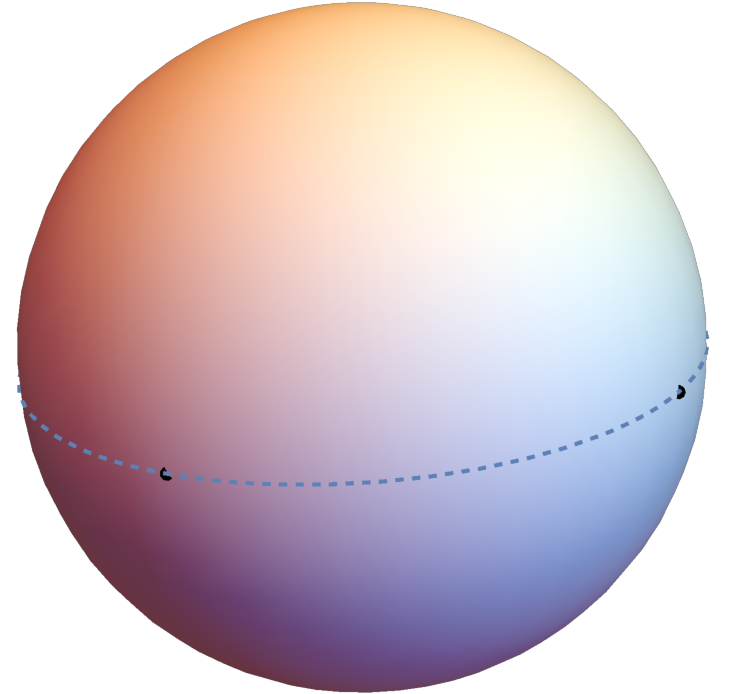
\includegraphics{Figures/S2CW.pdf}
\caption{Espacio $S^2$ construido utilizando el \refexample{S2CW}.}
\end{marginfigure}

De esta forma, tenemos que un espacio topológico no induce una descomposición
como CW-complejo de forma única. Si comparamos este proceso con el que
seguimos en el \refexample{Sn_CW}, tenemos que no tienen el mismo número de
células y sus $1$-esqueletos no son homeomorfos, de forma que no son
\textit{estructuras equivalentes}.

\begin{theorem}[Caracterización de CW-complejos finitos]\labthm{TCCWF}
Un espacio topológico compacto $X$ es un CW-complejo finito de dimensión $n$
si y sólo si podemos hallar una sucesión de subespacios
\[X^0 \subseteq X^1 \subseteq \dots \subseteq X^n=X\]
y una partición de subconjuntos
\[\{D_i^k:\; k=0,1,\dots,n; \;i=1,2,\dots,r_k\}\]
(llamada \textbf{descomposición celular}) tales que
\begin{enumerate}
\item existe un homeomorfismo relativo
\[h\colon (D^k,S^{k-1}) \to
(\overline{D^k_i},\overline{D^k_i}\backslash D^k_i)\]
para cada $i$ y $k$;
\item dado un $1 \leq k \leq n$, $\overline{D^k_i}\backslash D^k_i
\subseteq X^{k-1}$.
\end{enumerate}
\end{theorem}

Hagamos un par de incisos en este teorema.

\begin{itemize}
\item Observar que $\overline{D^k_i}\backslash(\overline{D^k_i}\backslash
D^k_i)=D^k_i$. Aplicando el teorema anterior, se sigue que $D^k_i$ es
homeomorfo a una bola abierta de $\mb{R}^k$. Esto implica que las $n$-células
son conexas, compactas y abiertas para todo $n > 0$.
\item La condición de compacidad viene dada porque la adjunción de espacios
compactos es compacto, pero ninguna de las otras condiciones garantizan que
$X$ sea compacto.
\end{itemize}

\begin{example}
\begin{enumerate}
\item Este teorema proporciona otra forma de ver que $S^n$ admite una
estructura de CW-complejo: para $n=1$, sea $f\colon [0,2\pi] \to \mb{R}^2$ la
aplicación $f(t)=(\cos t,\sin t)$. Tenemos que $X=S^1$ admite una estructura
de CW-complejo tomando
\begin{align*}
X^0&=\{(1,0)\}; 	& X^1&=S^1;\\
D^0&=\{(1,0)\}; 	& D^1&=f(]0,1[]);
\end{align*}
Para $n=2$, sea $g\colon [0,1]\times [0,1] \to \mb{R}^3$ la aplicación
\[g(u,v)=(\cos(2\pi u)\cos(2\pi v),\cos(2\pi u)\sin(2\pi v),\sin(2\pi u))\]
Entonces, $Y=S^2$ admite una estructura de CW-complejo tomando
\begin{align*}
Y^0		&=\{(1,0,0)\}; 	& D^0&=\{(1,0,0)\};\\
Y^1 	&=S^1 			&
D^2_1	&=g([0,1]\times(]0,3/4[\cup]3/4,1[));\\
D^1 	&=g([0,1]\times\{0\});	&
D^2_2	&=g([0,1]\times(]1/4,3/4[]));
\end{align*}
\item El segmento $I$ admite una estructura de CW-complejo dada por la
descomposición celular $\{\{0\},\{1\},]0,1[\}$. En general, toda línea
poligonal formada por una cantidad finita de segmentos admite una estructura
trivial de CW-complejo.
\end{enumerate}
\end{example}

\begin{example}
\begin{enumerate}
\item El conjunto $A=\{1/n: n \in \mb{N}\}\cup \{0\}$ con la topología
inducida por la métrica usual de $\mb{R}$ no es un CW-complejo finito, porque
no es compacto.

\item El \textbf{pendiente hawaiiano} es un ejemplo de espacio topológico
compacto que no tiene estructura de CW-complejo. Si $C(\alpha,\beta)$ denota
la circunferencia de centro $\alpha \in \mb{R}^2$ y radio $\beta > 0$, se
define el pendiente hawaiiano como el espacio topológico
\begin{align*}
H=\bigcup_{n=1}^\infty C(\alpha_n,\beta_n) &&
\left(\alpha_n=\left(\frac{1}{n},0\right), \quad 
\beta_n=\frac{1}{n}\right)
\end{align*}
Intuitivamente, esto se debe a que tiene una cantidad infinita de anillos, y
cada uno tendría que ser una 1-célula independiente.
\end{enumerate}
\end{example}

\begin{marginfigure}
\resizebox{\textwidth}{!}{
\begin{tikzpicture}[scale=0.1]
\foreach \n in {4,...,20}
	\draw (\n,0) circle (\n cm);
\end{tikzpicture}
}
\caption{Primeras $16$ iteraciones del pendiente hawaiiano.}
\end{marginfigure}

\begin{proposition}\labprop{CWProd}
El producto de CW-complejos finitos es un CW-complejo finito.
\end{proposition}

\begin{proof}
Sean $\mc{C}=\{D_i^k:\; k=0,1,\dots,n; \;i=1,2,\dots,r_k\}$ y $\mc{D}=
\{\Delta_\ell^j:\; j=0,1,\dots,m; \;\ell=1,2,\dots,r_j\}$ respectivas
descomposiciones celulares de $X$ e $Y$. Queremos ver que el conjunto
\[\mc{E}=\{U\times V: U\in \mc{C}, V\in \mc{D}\}\]
forma una descomposición celular de $X\times Y$.

Claramente, los elementos de $\mc{E}$ son disjuntos dos a dos por
construcción. Veamos que forman un recubrimiento de $X\times Y$: 
\[X\times Y=
	\left(\bigcup_{U \in \mc{C}} U\right)\times
	\left(\bigcup_{V \in \mc{D}} V\right)=
	\bigcup_{\substack{U \in \mc{C}\\V \in \mc{D}}} U\times V\]

Para demostrar este resultado, aplicaremos el \refthm{TCCWF}: dados
$i,j,k,\ell$,
\begin{align*}
U&=(\overline{D^k_i\times \Delta^\ell_j})\backslash
	(D^k_i\times \hat D^\ell_j)=
	(\overline{D^k_i}\times \overline{\Delta^\ell_j})\backslash
	(D^k_i\times \hat D^\ell_j)=\\
	&=[(\overline{D^k_i}\backslash D^k_i)\times \overline{\Delta^\ell_j}]\cup
	[\overline{D^k_i}\times (\overline{\Delta^\ell_j}\backslash \Delta^\ell_j)]
\end{align*}
Sabemos por hipótesis que $(\overline{D^k_i}\backslash D^k_i) \subseteq
X^{k-1}$ y $\overline{\Delta^\ell_j}\backslash \Delta^\ell_j \subseteq
Y^{\ell-1}$, por lo que $U \subseteq (X\times Y)^{k+\ell-1}$. Esto prueba la
primera condición.

Pasemos a la segunda: sean $U \in \mc{C}$ y $V \in \mc{D}$. Si
\begin{align*}
f\colon (D^k,S^{k-1}) \to (\overline{U},\overline{U}\backslash U); &&
g\colon (D^\ell,S^{\ell-1}) \to (\overline{V},\overline{V}\backslash V)
\end{align*}
son homeomorfismos relativos, se tiene que
\[f\times g\colon (D^{k+\ell},S^{k+\ell-1}) \to
(\overline{V\times V},(\overline{U\times V})\backslash (U\times V))\]
es un homeomorfismo relativo.
\end{proof}

\begin{example}\labexample{CWlindro}
\begin{enumerate}
\item El cilindro con bordes se define como $C=S^1\times [0,1]$. Podemos
asignar una estructura de CW-complejo a $C$ usando una estructura prefijada
de $S^1$ y otra de $[0,1]$:

\begin{align*}
[0,1]
\begin{cases}
\text{0-células:}	&p=\{0\}\\
					&q=\{1\}\\
\text{1-células:}	&\alpha=]0,1[
\end{cases}
&&
S^1
\begin{cases}
\text{0-células:}	&r=\{(1,0)\}\\
\text{1-células:}	&\beta=S^1-r
\end{cases}
\end{align*}

Estas estructuras inducen la siguiente descomposición celular sobre el cilindro:
\[C \begin{cases}
\text{0-células:}	&p\times r, q\times r\\
\text{1-células:}	&\alpha \times r, p\times \beta, q\times \beta\\
\text{2-células:}	&\alpha \times \beta
\end{cases}\]

\item El toro se puede expresar como $S^1\times S^1$, por lo que admite una
estructura de CW-complejo finito.

Consideremos la siguiente descomposición celular de $S^1$:
\begin{align*}
S^1
\begin{cases}
\text{0-células:}	&p=\{(1,0)\}\\
\text{1-células:}	&\alpha=S^1-p
\end{cases}
&&
S^1
\begin{cases}
\text{0-células:}	&r=\{(1,0)\}\\
\text{1-células:}	&\beta=S^1-r
\end{cases}
\end{align*}

Estas estructuras inducen la siguiente descomposición celular sobre el toro:
\[S^1\times S^1
\begin{cases}
\text{0-células:}&p\times r\\
\text{1-células:}&\alpha \times r,p\times \beta\\
\text{2-células:}&\alpha \times \beta
\end{cases}\]
\end{enumerate}
\end{example}

\begin{marginfigure}
\resizebox{\textwidth}{!}{
\begin{tikzpicture}
\draw (2,0) circle (.9cm);
\draw (1.1,0) -- (-.1,0);
\draw (-1,0) circle (.9cm);
\end{tikzpicture}
}
\caption[1-esqueleto del cilindro.]{1-esqueleto del cilindro. Observar que se
puede retraer en una figura ocho.}
\end{marginfigure}

\begin{marginfigure}
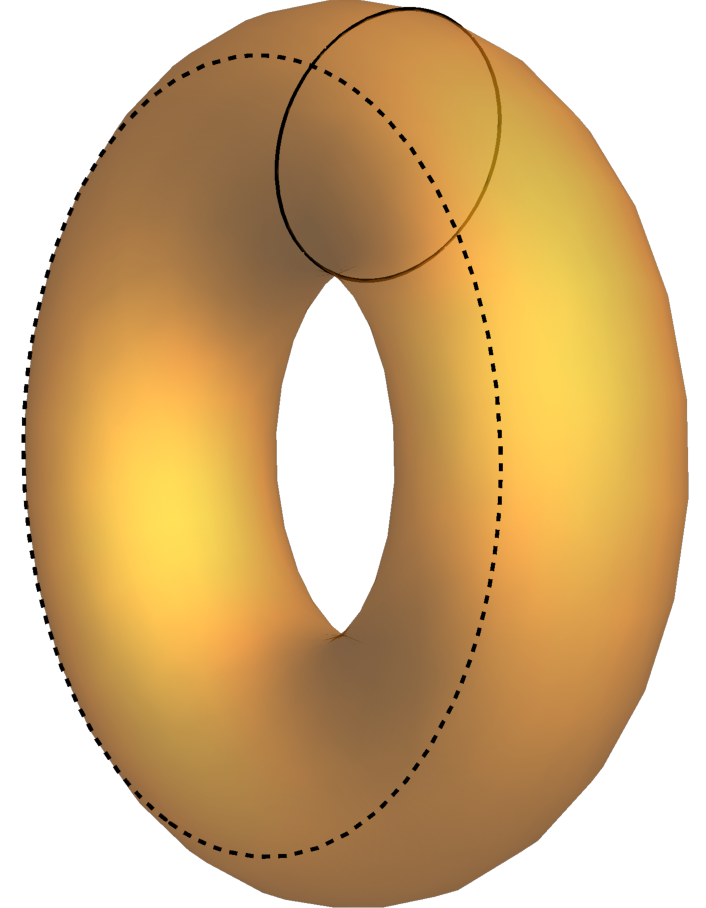
\includegraphics{Figures/ToroGeneradoresOrden1.pdf}
\caption{1-esqueleto del toro.}
\end{marginfigure}

\subsection{Subcomplejos}
Sea $X$ un CW-complejo finito y $\mc{C}$ una descomposición celular de $X$.
Decimos que un subespacio $A \subseteq X$ es un \textbf{subcomplejo} de $X$ si,
dado $D \in \mc{C}$, $D\cap A \neq \emptyset$ implica que $\overline{D}
\subseteq A$. Esta condición se puede expresar como que $A$ absorbe a todas
las células con las que entra en contacto.

Todo subcomplejo de un cierto complejo $X$ conforma un subespacio cerrado.
Además, aplicando el \refthm{TCCWF}, todo subcomplejo es un complejo en sí
mismo. En particular, todos los $k$-esqueletos de $X$ son subcomplejos.

\begin{proposition}
Si $A$ es un subcomplejo de un CW-complejo finito $X$, $A$ es un retracto por
deformación fuerte de algún entorno compacto de $A$ en $X$.
\end{proposition}

\begin{proof}
Sea $N$ el número de células que componen el espacio $X\backslash A$. Si
$N=0$, $X=A$, por lo que $A$ es un retracto por deformación fuerte de $X$ de
forma trivial y se sigue la tesis por compacidad de $X$.

Si $N=1$, existe una aplicación $f\colon S^{n-1} \to A$ continua tal que
$X=A\cup_f D^n$. En tal caso, podemos limitarnos a aplicar el
\reflemma{EntornoCompacto}.

Supongamos que el resultado es cierto para cualquier par de CW-complejos
finitos $(Y,B)$ tales que $Y\backslash B$ posee a lo sumo $N-1$ células, y sea
$(X,A)$ un par de CW-complejos tales que $X\backslash A$ tiene exactamente $N$
células. Si $D^m_i$ es una célula de $X\backslash A$ de dimensión máxima, se
define el subespacio $Y=X\backslash D^m_j$.

Queremos ver que $Y$ es un subcomplejo de $X$. Como $D^m_i$ es una célula de
dimensión máxima, todas las células de $X\backslash A$ tienen dimensión $m$ o
menos; de esta forma, toda célula de $X$ con dimensión mayor que $m$ forma
parte del subcomplejo $A$. En consecuencia, si $D^k_j$ es una célula de $Y$,
se tiene que $D^k_j \subset A$ ó $k \leq m$.

Si $D^k_j \subset A$, $\overline{D^k_j} \subseteq A$ por ser $A$ un
subcomplejo de $X$, de forma que
\[D^m_i \cap \p D^k_j \subseteq D^m_i \cap A=\emptyset\]
En cambio, si $k \leq m$, se tiene por \refthm{TCCWF} que
\[\p D^k_j=\overline{D^k_j}\backslash D^k_j\subseteq X^{k-1}\]
Dado que $k-1 < m$, se cumple una vez más que $D^m_i \cap \p D^k_j=\emptyset$.
Se sigue que $Y$ es subcomplejo de $X$.

Dado que $A$ es un subcomplejo de $X$ y $D^m_i \subset X\backslash A$, $A\cap
D^m_i=\emptyset$, por lo que es un subcomplejo de $Y$. Como $Y$ tiene una
célula menos que $X$, el par $(Y,A)$ verifica la hipótesis de inducción, por
lo que existe un entorno $U_1$ compacto de $A$ en $X$ tal que $A$ es un
retracto por deformación fuerte de $U_1$.

Sea $f\colon S^{m-1} \to Y$ una aplicación continua tal que $X=Y\cup_f D^m$.
Podemos hallar un homeomorfismo relativo
\[\phi\colon (D^m,S^{m-1}) \to
	(\overline{D^m_i}, \overline{D^m_i}\backslash D^m_i)\]
que extienda a $f$ de forma continua. Como $U_1$ es compacto en $Y$ y $\phi$
es un homeomorfismo, $\phi^{-1}(U_1)$ es un compacto de $S^{m-1} \subset D^m$.
Si
\begin{diag}
r\colon D^m\backslash\{0\} \arrow[r] & S^{m-1}\\[-8mm]
x \arrow[maps to,r]& \frac{x}{\|x\|}
\end{diag}
es la retracción radial, el conjunto
\[V=\{\phi(x): x \in D^m,\; \|x\| \geq 1/2,\; r(x) \in \phi^{-1}(U_1)\}\]
también es compacto.

Veamos cómo se construye el conjunto $V$: las células se adhieren al
CW-complejo por el borde, por lo que podemos pensar que la aplicación $\phi$
abomba $D^m$ para darle forma de hemisferio y pegarlo a $Y$ por la línea del
ecuador. Se tiene entonces que $X=Y\cup \phi(D^m)$ (ver \reffig{ECompacto1}).

Dado que $Y\cap \phi(D^m)=f(S^{m-1})$, $\phi^{-1}(U_1)=f^{-1}(U_1)$ está
contenido en $S^{m-1}$. En particular, $x$ no tiene por qué estar en
$\phi^{-1}(U_1)$, por lo que lo retraemos mediante una aplicación adicional.
Finalmente, elegimos sólo los puntos que están entre las esferas concéntricas
de radios $1/2$ y $1$ (ver \reffig{PhiMenos1V}).

El conjunto $U_1 \cap V$ es un retracto por deformación de $V$, y $A$ es un
retracto por deformación de $U_1$, de forma que $A$ será un retracto por
deformación de $U_1 \cup V$ (ver \reffig{ECompacto2}).

\begin{marginfigure}
\begin{subfigure}[b]{\textwidth}
\resizebox{\textwidth}{!}{
\begin{tikzpicture}

%Esta instrucción colorea arcos "gorditos" de circunferencia
\fill[cyan!50] (45:.5) arc[start angle=45, end angle=-45, radius=.5] -- (-45:1)
	arc[start angle=-45, end angle=45, radius=1] -- cycle;
\fill[cyan!50] (135:.5) arc[start angle=135, end angle=225, radius=.5] -- (225:1)
	arc[start angle=225, end angle=135, radius=1] -- cycle;


\draw[to-to] (1.5,0) -- (-1.5,0);
\draw[to-to] (0,1.5) -- (0,-1.5);

\draw[dashed] (0,0) circle (1 cm) circle (.5 cm);

%Scope y clip cortarán las rectas donde se acaben las circunferencias
\clip (0,0) circle (1 cm);
\draw[dashed] (1,1) -- (-1,-1);
\draw[dashed] (1,-1) -- (-1,1);


\end{tikzpicture}
}
\caption{\labfig{PhiMenos1V} El conjunto $\phi^{-1}(V)$ corresponde a la
región coloreada. $\phi^{-1}(U_1)$ son los puntos de la región coloreada que
recaen sobre la esfera de radio $1$.}
\end{subfigure}
\begin{subfigure}[b]{\textwidth}
\resizebox{\textwidth}{!}{
\begin{tikzpicture}

\draw[dashed, fill=cyan!50] (1.5,2) circle (1cm);

\begin{scope}
\clip 	(0,0) .. controls (1,-1) and (2,-1) ..
		(3,0) .. controls (4,1) and (2,2) ..
		(3,4) .. controls (2,4) and (1,3) ..
		(0,4) .. controls (-1,3) and (1,2) ..
		(0,0);

\draw[pattern=north east lines]
	(0,1.5) .. controls (1,3.5) and (2,1.5) .. (4,4.5) --
	(4,4) .. controls (2,1) and (1,3) .. (0,1);

\draw[very thick] (4,4) .. controls (2,1) and (1,3) .. (0,1);
	
\draw[pattern=north east lines]
	(4,4) .. controls (2,1) and (1,3) .. (0,1) --
	(0,.5) .. controls (1,2.5) and (2,.5) .. (4,3.5);
\end{scope}

\draw (3.25,2.75) node {$A$};
\draw (0,1) -- (-.2,1) -- (-.2,2) -- (0,2);
\draw (-.6,1.5) node {$U_1$};

\draw 	(0,0) .. controls (1,-1) and (2,-1) ..
		(3,0) .. controls (4,1) and (2,2) ..
		(3,4) .. controls (2,4) and (1,3) ..
		(0,4) .. controls (-1,3) and (1,2) ..
		(0,0);

\end{tikzpicture}
}
\caption{Representación de los conjuntos $A$, $U_1$ y la bola $\phi(D^m)$ en
	$Y$.}
\end{subfigure}
\begin{subfigure}[b]{\textwidth}
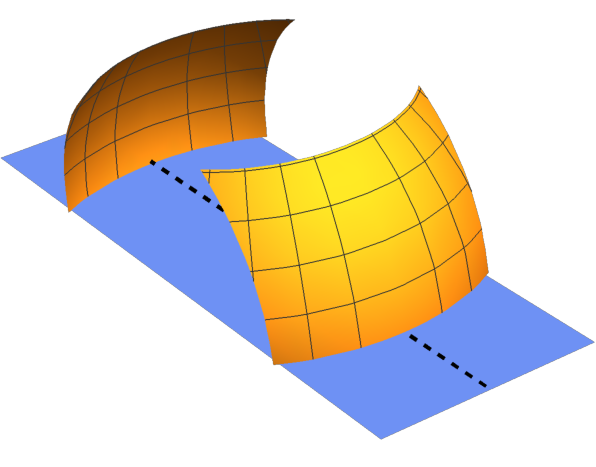
\includegraphics{Figures/ECompacto2.pdf}
\caption{\labfig{ECompacto2} Podemos retraer $V$ (superficies arqueadas) en
$U_1$ (banda plana) y $U_1$ en $A$ (línea discontinua).}
\end{subfigure}
\caption{Pasos ilustrados de la demostración.}
\end{marginfigure}

Ya sabemos que $U_1 \cup V$ se puede retraer en $A$. Dado que es unión de
compactos, es trivialmente compacto, de forma que habremos terminado la
demostración si podemos probar que $U_1 \cup V$ es entorno en $X$ de $A$.

Sea $y \in \Int_Y(U_1)$. Si $y \not\in V$, $y \in \Int_X(U_1)$
(repersentado como una banda en la ilustración \ref{ECompacto2}), por lo que
también estará en $\Int_X(U_1 \cup V)$.

Si $y \in V$, se tiene que $y \in \overline{D^m_i}\backslash D^m_i=
\phi(D^m\backslash \p D^m)=f(S^{m-1})$. Por otro lado,
$\phi^{-1}(\Int_Y(U_1))$ es un abierto de $S^{m-1}$ que contiene a
$\phi^{-1}(y)$ (por cómo se define $V$), de forma que 
\[\phi^{-1}(y) \in \Int_{S^{m-1}}\phi^{-1}(V) \implies y \in
\Int_{\overline{D^m_i}}(V)\]
Dado que $D^m_i$ es una célula de $X$, se sigue que $y \in
\Int_X(U_1\cup V)$.

Como $U_1$ es un entorno de $A$ en $Y$,
\[A \subseteq \Int_Y(U_1)\subseteq \Int_X(U_1\cup V)\]
por lo que $U_1\cup V$ es entorno de $A$ en $X$. Pero eso es lo que nos
quedaba por demostrar.
\end{proof}

\section{Grupos de homología celular}
\begin{corollary}\label{HomoCelular}
Si $X$ es un CW-complejo finito y $X^k$ es el $k$-esqueleto de $X$,
\[H_j(X^k,X^{k-1})=0 \quad \forall j \neq k\]
Además, $H_k(X^k,X^{k-1})$ es un grupo abeliano libre con un generador por
cada $k$-célula de $X$, conocido como el \textbf{grupo de homología celular}
de orden $k$.
\end{corollary}

\begin{proof}
Sabemos que $X^{k-1}$ es un subcomplejo de $X^k$. Por la proposición anterior,
existe un entorno compacto $U \subseteq X^k$ de $X^{k-1}$ tal que $X^{k-1}$
es un retracto por deformación fuerte de $U$.

Como $X$ es un CW-complejo finito, podemos hallar un homeomorfismo relativo
\[\phi: (\mc{D}^k, \mc{S}^{k-1}) \longrightarrow (X^k,X^{k-1})\]
utilizando los homeomorfismos $h$ que nos proporciona el teorema de
caracterización de CW-complejos finitos. Aplicando el teorema del
homeomorfismo relativo, se sigue que 
\begin{align*}
H_*(X^k,X^{k-1}) &\cong H_*(\mc{D}^k,\mc{S}^{k-1}) \cong 
	\sum^r_{i=1} H_*(D_i^k, S_i^{k-1}) \\
	& \cong \sum^r_{i=1} \tilde{H}_*(S^k) \cong
	\tilde{H}_*(S^k)^r \cong
	\begin{cases}
	\mb{Z}^r&\text{ si }p=k\\
	0&\text{ si no}
	\end{cases}
\end{align*}
\end{proof}

\begin{example}
Vamos a calcular la homología de la rosa de $p$ pétalos utilizando los grupos
de homología celular. Por la proposición \refprop{HomoCW},
\[H_j(B_p)\cong H_j(\{\star\})=0\]
para todo $j > 1$. Para $j=1$,
\[H_1(B_p)\cong \tilde{H}_1(B_p)\cong H_1(B_p,\{\star\})\]
Dado que $\{\star\}$ es el $0$-esqueleto de $B_p$, que tiene $p$ $1$-células, se
tiene que dicho grupo es isomorfo a $\mb{Z}^p$.
\end{example}

\section{Homología de la $n$-rosa}
Para $j=1,\dots,p$, sea $f_j\colon \p D^n \to \{\star\}$ la aplicación
constante. Se define la $n$-rosa de $p$ pétalos como la adjunción
\[X=B^n_p=\{\star\}_{f_1,\dots,f_p}\]

Por el corolario \ref{HomoCelular}, sabemos que $H_n(X^n,X^{n-1})\cong 
\mb{Z}^p$ y\\ $H_m(X^n,X^{n-1})=0$ para todo $m\neq n,0$. Sin embargo, $X^{n-1}
=X^0=\{\star\}$, por lo que
\begin{align*}
\mb{Z}^p\cong H_n(X,X^{n-1})=\tilde H_n(X);\\
0=H_m(X,X^{n-1})=\tilde H_m(X); && (m\neq n)
\end{align*}

\begin{theorem}\labthm{nrosa}
\[\tilde H_m(B^n_p)\cong
\begin{cases}
\mb{Z}^p & \text{si $m=n$}\\
0 & \text{si $m\neq n$}
\end{cases}\]
\end{theorem}

Al igual que pasaba con la $1$-rosa, cada pétalo que adjuntamos aporta un nuevo
generador, sólo que en este caso es la clase de un $n$-símplice singular.

\subsection{Rosa mixta}
¿Qué pasaría si mezcláramos pétalos de diferentes dimensiones? Intuitivamente,
cada pétalo de dimensión $k$ debería añadir un generador de orden $k$.

Sea $\alpha=(\alpha_1,\dots,\alpha_n) \in \mb{N}^n$. Si $f\colon \{\star\} \to
\{\star\}$ es la identidad, definimos
\[B_\alpha:=\{\star\}\cup_f B^1_{\alpha_1}\cup_f B^2_{\alpha_2}\cup_f \dots
\cup_f B^n_{\alpha_n}\]
siendo $B^k_0=\{\star\}$.

\begin{marginfigure}
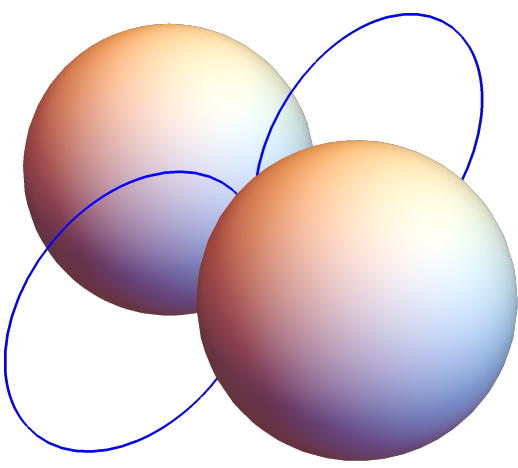
\includegraphics{Figures/B22.png}
\caption{Ejemplo de rosa mixta $B_{(2,2)}$.}
\end{marginfigure}

\begin{theorem}\footnote{Este resultado está basado en una conversación que
tuve con mi directora del TFG, pero no pensé en añadirlo en su momento.}
\labthm{RosaMixta}
Dado $\alpha \in \mb{N}^n$,
\[H_m(B_\alpha)\cong
\begin{cases}
\mb{Z}			& \text{si $m=0$}\\
\mb{Z}^{\alpha_i} 	& \text{si $m=i$}\\
0				& \text{si $m > n$}
\end{cases}\]
\end{theorem}

\marginnote[-2.2cm]{
\begin{kaobox}[frametitle=Idea de la demostración]
\begin{itemize}
\item Probamos que la tesis se cumple cuando la rosa tiene $k_1$ pétalos de
dimensión $1$ (ya lo hemos hecho).
\item Suponemos que la tesis se cumple cuando la rosa tiene $k_1$ pétalos de
dimensión $1$, $k_2$ pétalos de dimensión $2$, y así hasta dimensión $n-1$.
\item Probamos que, como consecuencia, la tesis se cumple cuando añadimos $k_n$
pétalos de dimensión $n$.
\end{itemize}

Esta prueba puede ser conceptualmente engorrosa, así que es recomendable tratar
de hacer primero ejemplos para $n=2,3,4$.
\end{kaobox}
}

\begin{proof}
Si $\alpha=(\alpha_1,\dots,\alpha_n)$, procedemos por inducción sobre $n$. Si
$n=1$, $B_\alpha$ es una $1$-rosa de $\alpha_1$ pétalos, y la tesis se cumple
por \refthm{nrosa}.

Sea $\alpha'=(\alpha_1,\dots,\alpha_{n-1})$, y $X=B_{\alpha'}$. Supongamos que
la tesis se cumple para $X$ y sean $f_i\colon S^{n-1} \longrightarrow \{\star\}$
aplicaciones constantes. Tenemos entonces que
\[B_\alpha=X_{f_1\dots f_{\alpha_n}}\]

Por la \refprop{HomoCW}, si $(f_i)_*\colon \tilde H_{n-1}(S^{n-1})\to
H_{n-1}(\{\star\})=\{0\}$, se cumple lo siguiente:
\begin{enumerate}
\item Para todo $p\neq n,n-1$,
\[H_p(X_{f_1\dots f_{\alpha_n}})=H_p(X)\]
Por hipótesis de inducción, $H_p(X)\cong \mb{Z}^{\alpha_p}$ cuando $p < n-1$ y
$\{0\}$ cuando $p > n-1$.
\item Como $(f_i)_*$ va a parar a $\{0\}$ para todo $i$, $\im (f_i)_*=\{0\}$ y
\begin{align*}
H_{n-1}(X_{f_1\dots f_{\alpha_n}})&\cong
	\frac{H_{n-1}(X_{f_1\dots f_{\alpha_n-1}})}{\im (f_{\alpha_n})_*}\cong
	H_{n-1}(X_{f_1\dots f_{\alpha_n-1}})\cong\\
	&\cong \frac{H_{n-1}(X_{f_1\dots f_{\alpha_n-2}})}{\im (f_{\alpha_n-1})_*}\cong
	H_{n-1}(X_{f_1\dots f_{\alpha_n-2}})\cong\\
	&\cong \dots \cong H_{n-1}(X)
\end{align*}
Por hipótesis de inducción una vez más, ésto es $\mb{Z}^{\alpha_{n-1}}$.
\end{enumerate}

El tercer ítem requiere que hagamos inducción sobre el número de pétalos de
dimensión $n$\footnote{Al principio, pensé que era necesario tratar este
resultado como una \emph{doble inducción}, así que decidí leer sobre el tema.
Si bien he conseguido reducirlo a una inducción aislada dentro de otra, creo
que es un tema interesante, así que he decidido escribir un pequeño apéndice
sobre el tema.}. Dado un espacio $Y$ arbitrario, sabemos por la
\refprop{HomoCW} que la secuencia
\[0 \longrightarrow H_n(Y) \longrightarrow H_n(Y_{f})
\longrightarrow \ker f_*\longrightarrow 0\]
es exacta. En particular, $\ker f_*=\tilde H_{n-1}(S^{n-1})\cong \mb{Z}$ por el
\labthm{HRelSn}, por lo que
\begin{equation}
\mb{Z}\cong \frac{H_n(Y_f)}{H_n(Y)} \label{ExactaZ}
\end{equation}
En este caso, $H_n(X)=\{0\}$ por hipótesis de inducción, por lo que
$H_n(X_{f_1})\cong \mb{Z}$.

Supongamos que $H_n(X_{f_1\dots f_{\alpha_n-1}})\cong \mb{Z}^{\alpha_n-1}$.
Usando \eqref{ExactaZ}, concluimos que
\[H_n(X_{f_1\dots f_{\alpha_n}})\cong H_n(X_{f_1\dots f_{\alpha_n-1}})\oplus
\mb{Z}\cong \mb{Z}^{\alpha_n}\]
concluyendo así ambas inducciones. Se sigue la tesis.
\end{proof}

\setchapterpreamble[u]{\margintoc}

\chapter{Homología de las superficies compactas}
Según el teorema de clasificación de superficies compactas, toda superficie
compacta y conexa es homeomorfa a $S^2$, a la suma conexa de $n$ toros o a la
suma conexa de $n$ planos proyectivos. Entre otras cosas, eso hace que las
componentes conexas de una superficie sean arcoconexas, dado que la
arcoconexión es una propiedad topológica.

Si llamamos $S_1,\dots,S_n$ a las componentes conexas de $S$, se tiene que
\[H_*(S)\cong \sum^n_{i=1}H_*(S_i)\]
por lo que podemos suponer a efectos de homología que $S$ es arcoconexa.

Por limitaciones de tiempo, nos restringiremos al caso de las superficies
orientables, que es más breve.

\subsection{Homología del $n$-toro}
\marginnote[-2.2cm]{
\begin{kaobox}[frametitle=Suma conexa de variedades]
Sea $X$ un espacio topológico Hausdorff y 2AN. Decimos que $X$ es una
$n$-variedad si, dado $p \in X$, existe un entorno abierto $U \subset X$ de
$p$ que sea homeomorfo a una bola abierta de $\mb{R}^n$.

Dadas dos $n$-variedades $X$ e $Y$, la suma conexa se define como
\[X\#Y=(X\backslash U)\cup_f (Y\backslash V)\]
siendo $U\subset X$, $V \subset Y$ abiertos y $f\colon \p U \to \p V$ continua.
\end{kaobox}
}
El $n$-toro (que denotaremos como $T_n$) se define como la suma conexa de $n$
toros. Podemos hacer la suma conexa de los representantes llanos, en cuyo caso
obtenemos una superficie como la que se puede ver en la \reffig{Bitoro}.

Si eliminamos el interior de $T_n$, la figura resultante será $B^1_{2n}$.  Si
$\gamma(t)=e^{2\pi i\theta}$, consideramos una aplicación $f\colon S^1\to
B_{2n}^1$ tal que
\[c_j=(f\circ\gamma)\left(\frac{j-1}{2n},\frac{j}{2n}\right)\]
es igual a cada uno de los pétalos de $B^1_{2n}$, con $j=1,\dots,2n$. Tenemos
entonces que $T_n=(B_{2n})_f$ (ver \reffig{Bitoro}). 

\marginnote[-2.2cm]{
\begin{kaobox}[frametitle=Ejercicio]
Comprueba que la cadena singular $c$ que estamos definiendo verifica que
$f([c])=0$ para $n=1,2,3$. Para $n=2$, puedes usar la \reffig{Bitoro} como
referencia; para $n=1,3$, es bueno dibujar el $n$-toro llano correspondiente.
\end{kaobox}
}

Vamos a estudiar la aplicación $f_*: \tilde{H}_1(S^1) \to H_1(B^1_{2n})$. El
grupo $\tilde{H}_1(S^1)$ tiene un único generador, $[c]$. Como representante
$c$, podemos elegir cualquier camino que dé una vuelta completa a $S^1$ (si no
da una vuelta completa, lo podemos contraer en un punto, por lo que está en la
clase del $0$). En particular, podemos elegir
\[c=\phi_1+\phi_2-(\phi_3+\phi_4)+\dots...+
	\phi_{2n-3}+\phi_{2n-2}-(\phi_{2n-1}+\phi_{2n})\]
donde $\phi_j(\sigma_1)=c_j$. Esta elección verifica que $f([c])=0$. Por tanto,
\begin{align*}
\im f_*=\{0\}; && \ker f_*=\tilde H_1(S^1)\cong \mb{Z}
\end{align*}

Por la proposición \refprop{CWHomo}, $H_p(T_n)\cong H_p(B^1_{2n})=0$ para todo
$p > 2$ y $H_1(T_n) \cong H_1(B_{2n})\cong \mb{Z}^{2n}$. Sólo nos queda
calcular el grupo de homología de orden 2:
\[0 \longrightarrow H_2(B^1_{2n}) \longrightarrow H_2(T_n) \longrightarrow
\tilde{H}_1(S^1) \longrightarrow 0\]
Dado que $H_2(B^1_{2n})=0$, se tiene por exactitud que
\[H_2(T_n) \cong \tilde{H}_1(S^1) \cong \mb{Z}\]

\begin{marginfigure}
\resizebox{\textwidth}{!}{
\begin{tikzpicture}
%Octógono
\draw[fill=green!50] (1,0) -- (2,0) -- (3,1) -- (3,2) -- (2,3) --
				(1,3) -- (0,2) -- (0,1) -- (1,0);

%La línea a través de la cual hacemos la suma conexa
\draw[dashed] (1,0) -- (2,3);

%Identificación de los lados
%c1
\draw[-stealth] (1,0) -- (1.5,0);
\draw (1.5,-.25) node {$c_1$};

%c2
\draw[-stealth] (2,0) -- (2.3,.3);
\draw[-stealth] (2.3,.3) -- (2.7,.7);
\draw (2.75,.25) node {$c_2$};

%c3
\draw[-stealth] (3,1) -- (3,1.5);
\draw (3.25,1.5) node {$c_3$};

%c4
\draw[-stealth] (3,2) -- (2.7,2.3);
\draw[-stealth] (2.7,2.3) -- (2.3,2.7);
\draw (2.75,2.75) node {$c_4$};

%c5
\draw[-stealth] (2,3) -- (1.75,3);
\draw[-stealth] (1.75,3) -- (1.5,3);
\draw[-stealth] (1.5,3) -- (1.25,3);
\draw (1.5,3.25) node {$c_5$};

%c6
\draw[-stealth] (1,3) -- (.8,2.8);
\draw[-stealth] (.8,2.8) -- (.6,2.6);
\draw[-stealth] (.6,2.6) -- (.4,2.4);
\draw[-stealth] (.4,2.4) -- (.2,2.2);
\draw (.25,2.75) node {$c_2$};

%c7
\draw[-stealth] (0,2) -- (0,1.75);
\draw[-stealth] (0,1.75) -- (0,1.5);
\draw[-stealth] (0,1.5) -- (0,1.25);
\draw (-.25,1.5) node {$c_7$};

%c8
\draw[-stealth] (0,1) -- (.2,.8);
\draw[-stealth] (.2,.8) -- (.4,.6);
\draw[-stealth] (.4,.6) -- (.6,.4);
\draw[-stealth] (.6,.4) -- (.8,.2);
\draw (.25,.25) node {$c_8$};
\end{tikzpicture}
}
\resizebox{\textwidth}{!}{
\begin{tikzpicture}
\draw[fill=green!50] (0,0) -- (0,2) -- (2,2) -- (2,0) -- (0,0);
\draw[dashed] (1,2) -- (2,1);
\draw (1,1) node {$T_1$};
\draw (2.3,1.5) node {$U$};

\draw[fill=green!50] (4,0) -- (4,2) -- (6,2) -- (6,0) -- (4,0);
\draw[dashed] (4,1) -- (5,2);
\draw (5,1) node {$T_1$};
\draw (3.7,1.5) node {$V$};

\begin{scope}
\clip (1,2) -- (5,2) -- (4,1) -- (2,1) -- (1,2);
\draw[pattern=north east lines] (1,1) -- (1,2) -- (2,2) -- (2,1) -- cycle;
\draw[pattern=north west lines] (4,1) -- (4,2) -- (6,2) -- (6,1) -- cycle;
\end{scope}

\draw[-stealth] (1.5,2.25) .. controls (2.5,2.75) and (3.5,2.75) .. (4.5,2.25);
\draw (3,2.25) node {$f$};
\end{tikzpicture}
}
\caption[Bitoro llano.]{\labfig{Bitoro} Bitoro llano. Los lados con el mismo
número de cabezas de flecha se identifican entre sí. La línea discontinua
separa los dos toros que lo conforman.}
\end{marginfigure}

De esta forma, \[H_n(T_n)\cong
\begin{cases}
\mb{Z}^{2n}	&\text{ si $n =1$}\\
\mb{Z}		&\text{ si $n=0,2$}\\
0			&\text{ si no}
\end{cases}\]

\begin{theorem}
Sea $S$ una superficie compacta y orientable con $\alpha$ componentes
conexas. Existe un $n \geq 0$ tal que
\[H_q(S)\cong \begin{cases}
\mb{Z}^{2n\alpha}	&\text{ si $q =1$}\\
\mb{Z}^\alpha		&\text{ si $q =0,2$}\\
0   				&\text{ si no}
\end{cases}\]
El valor $n$ se denomina \textbf{género} de la superficie.
\end{theorem}

\subsection{Espacio proyectivo real}
\begin{definition}
Dados $v,w \in S^n$, diremos que $v \sim w$ si $w=\pm v$. Definimos el espacio
proyectivo real $\mb{R}P^n$ como el cociente $S^n/\sim$.
\end{definition}

El espacio proyectivo real se puede entender como el espacio topológico
cuyos puntos son las rectas de $\mb{R}^{n+1}$ que pasan por cero. Una forma
de entender $\mb{R}P^n$ es como el menor espacio compacto que contiene a
$\mb{R}^n$ como subespacio.

\begin{kaobox}[frametitle=¿Qué significa que $\mb{R}^n$ sea subespacio de
$\mb{R}P^n$?]
Sea $\pi\colon S^n \to \mb{R}P^n$ la proyección canónica. Dado un punto
$[x] \in \mb{R}P^n$, $\pi^{-1}([x])=\{x,-x\}$. Decimos entonces que
\emph{$S^n$ cubre a $\mb{R}P^n$ dos veces}.

Sea $B^n$ la bola abierta unidad de $\mb{R}^n$. La aplicación $f\colon
\mb{R}^n \to B^n$ dada por
\[f(x)=\frac{x}{1+\|x\|}\]
es un homeomorfismo. Por otro lado,
\begin{diag}
g\colon B^n \arrow[r] & S^n\\[-8mm]
x \arrow[r, maps to] & \left(x,\sqrt{1-\|x\|^2}\right)
\end{diag}
es un homeomorfismo que envía a $B^n$ en el hemisferio norte de $S^n$ (menos
el ecuador). Si $E^n_+=g(B^n)$, $\pi|_{E^n_+}$ es un homeomorfismo (observa
que $S^n$ es compacto y $\mb{R}P^n$ es Hausdorff). Si conectamos todas estas
aplicaciones, obtenemos
\begin{diag}
h\colon \mb{R}^n \arrow{r}{f} & B^n \arrow{r}{g} & E^n_+ \arrow{r}{\pi}
	&\mb{R}P^n
\end{diag}
Una consecuencia de nuestro proceso es que $h$ es un homeomorfismo sobre su
imagen; sin embargo, no es sobreyectiva, por lo que su imagen es un
subespacio de $\mb{R}P^n$. Ya que $\mb{R}^n$ es homeomorfo a $h(\mb{R}^n)$,
decimos por asociación que $\mb{R}^n$ es un subespacio de $\mb{R}P^n$.
\end{kaobox}

Otra posible interpretación, más en línea con la geometría sintética, es que
$\mb{R}P^n$ es una extensión de $\mb{R}^n$ donde todo par de rectas paralelas
se cruzan en \emph{el infinito}. Esta interpretación da lugar a la geometría
proyectiva, cuyo objetivo es diseñar técnicas geométricas que no dependan
de la perspectiva. Los lectores interesados pueden ver una aplicación de
geometría proyectiva en \cite{Numberphile}.

Podemos identificar $S^n$ con el subespacio de $S^{n+1}$ de ecuación
$x_{n+2}=0$ (el ecuador), en cuyo caso tenemos la inclusión $i\colon
S^n \hookrightarrow S^{n+1}$. Esta aplicación induce una inclusión sobre los
cocientes,
\[j\colon \mb{R}P^n \hookrightarrow \mb{R}P^{n+1}\]
En el cuadro anterior, vimos que la aplicación $\pi\circ g$ lleva a $B^{n+1}$
en un subespacio de $\mb{R}P^{n+1}$. Dado que $D^{n+1}=\overline{B^{n+1}}$,
$\pi\circ g$ induce una aplicación sobreyectiva $G\colon D^{n+1} \to
\mb{R}P^{n+1}$, que a su vez da lugar a
\[G\cup j\colon D^{n+1}\cup \mb{R}P^n \longrightarrow \mb{R}P^{n+1}\]

Dado un $p \in \mb{R}P^{n+1}$, $G^{-1}(p)$ puede ser un único punto de
$D^{n+1}\backslash S^n$ o un par $\{x,-x\}$ en $S^n$. Usando el
\reflemma{RepAdj}, concluimos que $\mb{R}P^{n+1}$ es homeomorfo al espacio
de adjunción $\mb{R}P^n_\pi$.

Para $n=1$, $\mb{R}P^1$ es homeomorfo a $S^1$, por lo que ambos espacios
tienen el mismo tipo de homología. Para $n=2$, la proyección canónica
$\pi\colon S^1 \to \mb{R}P^1$ induce una aplicación en homología $\pi_*\colon
\tilde H_1(S^1) \to H_1(\mb{R}P^1)$.

Sean $\alpha,\beta\colon I \to S^1$ las aplicaciones
\begin{align*}
\alpha(t)=(\cos \pi t, \sin\pi t); && \beta(t)=\alpha(t+1);
\end{align*}
Podemos identificar $\alpha$ y $\beta$ con $1$-símplices singulares, en cuyo
caso $[\alpha+\beta]$ es un generador de $\tilde H_1(S^1)$. Usando propiedades
de trigonometría elemental, observamos que $\pi\circ\alpha=\pi\circ\alpha$,
por lo que
\[\pi_*([\alpha+\beta])=2[\alpha]\]
y $\im \pi_*\cong 2\mb{Z}$. Usando que $\mb{Z}\cong\mb{Z}_2\times 2\mb{Z}$,
\[2\mb{Z}\cong \frac{\mb{Z}}{\ker\pi_*}
\cong\frac{2\mb{Z}\times \mb{Z}_2}{\ker \pi_*}\]
luego $\ker\pi_*\cong \mb{Z}_2$.

Usando la \refprop{HomoCW}, vemos que $H_p(\mb{R}P^2)=0$ para $p > 2$ y
\[H_1(\mb{R}P^2) \cong \frac{H_1(S^1)}{\im \pi_*}
				\cong \frac{\mb{Z}}{2\mb{Z}}=\mb{Z}_2\]
Para $n=2$, usaremos la exactitud del diagrama
\begin{diag}
0 \arrow[r]& H_2(S^1) \arrow[r]& H_2(\mb{R}P^2) \arrow[r]&
\ker \pi_* \arrow[r]& 0
\end{diag}
que es equivalente a
%La respuesta es 0


\chapter{Dos generaliazciones del toro}
\section{$W=S^2\times S^1$}
El toro de Clifford se define como $S^1\times S^1$, pero podemos reemplazar una de las dos copias de $S^1$ por $S^2$ para obtener una 3-variedad.
Como veremos, esta variedad tiene característica de Euler 0, pero no es homeomorfa a $S^3$ porque sus grupos de homología no son los mismos.

Considérese la aplicación
\[\funcio{f}{\mbR}{\mb{C}}{t}{e^{2\pi i t}}\] Se define el siguiente recubrimiento de $W$: \[U=S^2\times f([0,3/4]); \quad V=S^2 \times f([1/2,5/4])\] $S^2$ es un retracto por deformación de $U$ y de $V$, por lo que $H_*(U)\cong H_*(S^2)\cong H_*(V)$ Además, $S^2\sqcup S^2$ es un retracto por deformación fuerte de $U\cap V$, por lo que $$H_*(U\cap V)\cong H_*(S^2)^2$$

Consideremos la sucesión de Mayer-Vietoris asociada al par $\{U,V\}$: dado un $n > 3$,
\[\begin{array}{ccccccc}
H_n(U\cap V)&\xrightarrow{g_n}&H_n(U)\oplus H_n(V)	&\xrightarrow{h_n}	&H_n(W)		&\xrightarrow{\Delta_n}&H_{n-1}(U \cap V)\\
\downarrow&&\downarrow			&					&\downarrow	&					&\downarrow\\
0& \rightarrow&0			&\rightarrow			&H_n(W)		&\rightarrow			&0
\end{array}\]

Por exactitud, tenemos que $h_n$ es un isomorfismo, por lo que $H_n(W) \cong H_n(U)\oplus H_n(V)=0$. Pasemos a calcular $H_1(W)$:

\[\begin{array}{ccccccc}
H_0(U\cap V)&\xrightarrow{g_0}&H_0(U)\oplus H_0(V)	&\xrightarrow{h_0}	&H_0(W)&\longrightarrow &0\\
\downarrow&					&\downarrow			&					&\downarrow & &\downarrow\\
\mb{Z}^2& \rightarrow&\mb{Z}^2			&\rightarrow			&\mb{Z} & \rightarrow & 0		
\end{array}\]

Dado que $H_0(W)\cong \mb{Z}$, $\im h_0\cong \mb{Z}$, por lo que $\im g_0=\ker h_0\cong \mb{Z}$ y $\ker g_0\cong \mb{Z}$ en consecuencia. 

\[\begin{array}{ccccccc}
H_1(U)\oplus H_1(V)	&\xrightarrow{h_1}	&H_1(W)		&\xrightarrow{\Delta_1}&H_0(U \cap V)\\
\downarrow			&					&\downarrow	&					&\downarrow\\
0			&\rightarrow			&H_1(W)		&\rightarrow			&\mb{Z}^2
\end{array}\]

Por exactitud, se tiene que $\im \Delta_1=\ker g_0\cong \mb{Z}$ y que $\ker \Delta_1=\im h_1=0$. De aquí se sigue que $$H_1(W)\cong \mb{Z}$$

Nos falta calcular $H_2(W)$ y $H_3(W)$. Para ello, consideraremos la siguiente descomposición de $S^2\times S^1$: \[U'=\{(x,y,z) \in S^2: z \geq -1/2\}; \quad U=U'\times S^1\] \[V'=\{(x,y,z) \in S^2: z \leq 1/2\}; \quad V=V'\times S^1\] Se tiene que $S^1\times S^1=T$ es un retracto por deformación de $U\cap V$, por lo que $H_*(U\cap V) \cong H_*(T)$. Además, $S^1$ es un retracto por deformación de $U$ y $V$, por lo que \[H_*(U) \cong H_*(S^1) \cong H_*(V)\]

Considérese el siguiente tramo de la sucesión de Mayer-Vietoris asociada al par $\{U,V\}$: \[\begin{array}{ccccccc}
H_3(U)\oplus H_3(V)	&\xrightarrow{h_3}	&H_3(W)		&\xrightarrow{\Delta_3}&H_2(U \cap V)&\xrightarrow{g_3}&H_2(U)\oplus H_2(V)\\
\downarrow			&					&\downarrow	&					&\downarrow & & \downarrow\\
0			&\rightarrow			&H_3(W)		&\rightarrow			&\mb{Z} & \rightarrow & 0
\end{array}\]

Por exactitud, se tiene que $\Delta_3$ es un isomorfismo entre $H_2(U\cap V) \cong \mb{Z}$ y $H_3(W)$, por lo que \[H_3(W)\cong \mb{Z}\] Sólo queda por calcular el grupo de orden 2: la aplicación $$h_0: H_0(U) \oplus H_0(V) \longrightarrow H_0(W)$$ es un epimorfismo, por lo que su imagen es isomorfa a $\mb{Z}$ y su núcleo es también isomorfo a $\mb{Z}$ (por el primer teorema de isomorfia).

\[\begin{array}{ccccccc}
H_1(U)\oplus H_1(V)	&\xrightarrow{h_1}	&H_1(W)&\xrightarrow{\Delta_1}&H_0(U\cap V)&\xrightarrow{g_0}&H_0(U) \oplus H_0(V)\\
\downarrow&		&\downarrow		&	&\downarrow & 	&\downarrow\\
\mb{Z}^2	& \rightarrow	&\mb{Z}	&\rightarrow	&\mb{Z} & \rightarrow & \mb{Z}^2	
\end{array}\]

Sabemos que $\im g_0=\ker h_0 \cong \mb{Z}$, de forma que $\im \Delta_1=\ker g_0=0$. De aquí se sigue que $\im h_1=\ker \Delta_1\cong \mb{Z}$, por lo que $\ker h_1\cong \mb{Z}$. 

\[\begin{array}{ccccccc}
H_2(U)\oplus H_2(V)	&\xrightarrow{h_2}	&H_2(W)&\xrightarrow{\Delta_2}&H_1(U\cap V)&\xrightarrow{g_1}&H_1(U) \oplus H_1(V)\\
\downarrow&		&\downarrow		&	&\downarrow & 	&\downarrow\\
0& \rightarrow	&H_2(W)		&\rightarrow	&\mb{Z}^2 & \rightarrow & \mb{Z}^2	
\end{array}\]

Dado que $\im g_1=\ker h_1\cong \mb{Z}$, $\im \Delta_2=\ker g_1\cong \mb{Z}$. También se tiene que $\ker \Delta_2=\im h_2=0$ por exactitud, de forma que $$H_2(W)\cong \frac{H_2}{\ker \Delta_2}\cong \im \Delta_2\cong \mb{Z}$$

Concluimos que \[H_n(W)\cong\begin{cases}\mb{Z} & \mbox{ si }n < 4\\0 & \mbox{ si no}\end{cases} \implies\chi(W)=1-1+1-1=0\] Es decir, que la característica de Euler del espacio $W$ coincide con la de $S^3$, pero sus grupos de homología no son isomorfos. Dado que el grupo de homología es un invariante topológico, se tiene que $S_3$ no es homeomorfo a $W$.

\section{$T^3=S^1\times S^1 \times S^1$}
Considérese la siguiente descomposición de $T^3$, siendo $f$ la aplicación del ejemplo anterior: \[U=T\times f([0,3/4]); \quad V=T \times f([1/2,5/4])\] Se tiene que $T$ es un retracto por deformación de $U$ y de $V$, por lo que $H_*(U)\cong H_*(T) \cong H_*(V)$.
Por otro lado, $U\cap V=T\sqcup T$, por lo que \[H_*(U\cap V)\cong H_*(T_2)^2\]

Para $n > 3$, la sucesión de Mayer-Vietoris asociada al par $\{U,V\}$ da lugar a la siguiente sucesión exacta corta: \[\begin{array}{ccccccc}
H_n(U\cap V)&\xrightarrow{g_n}&H_n(U)\oplus H_n(V)	&\xrightarrow{h_n}	&H_n(T^3)		&\xrightarrow{\Delta_n}&H_{n-1}(U \cap V)\\
\downarrow&&\downarrow			&					&\downarrow	&					&\downarrow\\
0& \rightarrow&0			&\rightarrow			&H_n(T^3)		&\rightarrow			&0
\end{array}\] Por exactitud, se tiene que $H_n(T^3)\cong H_n(T)^2=0$. Sólo necesitamos calcular los casos $n=1,2,3$.

\[\begin{array}{ccccccc}
H_0(U\cap V)&\xrightarrow{g_0}&H_0(U)\oplus H_0(V)	&\xrightarrow{h_0}	&H_0(T^3)&\longrightarrow &0\\
\downarrow&					&\downarrow			&					&\downarrow & &\downarrow\\
\mb{Z}^2& \rightarrow&\mb{Z}^2			&\rightarrow			&\mb{Z} & \rightarrow & 0		
\end{array}\]

Dado que $H_0(W)\cong \mb{Z}$, $\im h_0\cong \mb{Z}$, por lo que $\im g_0=\ker h_0\cong \mb{Z}$ y $\ker g_0\cong \mb{Z}$ en consecuencia.

\[\begin{array}{ccccccc}
H_1(U)\oplus H_1(V)	&\xrightarrow{h_1}	&H_1(T^3)		&\xrightarrow{\Delta_1}&H_0(U \cap V)\\
\downarrow			&					&\downarrow		&						&\downarrow\\
\mb{Z}^4			&\rightarrow		&H_1(T^3)		&\rightarrow			&\mb{Z}^2
\end{array}\]

Se tiene por exactitud que $\im \Delta_1=\ker g_0\cong \mb{Z}$. Por el primer teorema de isomorfia, \[\frac{H_1(T^3)}{\ker \Delta_1} \cong \mb{Z}\] Necesitamos determinar el núcleo de $\Delta_1$ manualmente; no obstante, podemos calcular la imagen de $h_1$ en su lugar, que es más sencillo.
\\

Recordemos cómo se define $h_1$: \[\funcio{h_1}{H_1(T)^2}{H_1(T^3)}{([\alpha],[\beta])}{[\alpha]+[\beta]}\] Dado que $H_1(T)$ tiene dos generadores, existen 1-ciclos $a,b \in Z_1(T)$ y enteros $\lambda_1,\lambda_2,\mu_1,\mu_2$ tales que \[[\alpha]+[\beta]=\lambda_1[a]+\mu_1[b]+\lambda_2[a]+\mu_2[b]\] De aquí se sigue que \[\ker \Delta_1=\im h_1=\{\lambda[a]+\mu[b]: \lambda,\mu \in \mb{Z}\} \cong \mb{Z}^2\] por lo que $H_1(T^3)\cong \mb{Z}^3$.

\[\begin{array}{ccccccc}
H_2(U)\oplus H_2(V)	&\xrightarrow{h_2}	&H_2(T^3)&\xrightarrow{\Delta_2}&H_1(U\cap V)&\xrightarrow{g_1}&H_1(U) \oplus H_1(V)\\
\downarrow&		&\downarrow		&	&\downarrow & 	&\downarrow\\
\mb{Z}^2& \rightarrow	&H_2(T^3)		&\rightarrow	&\mb{Z}^4 & \rightarrow & \mb{Z}^4
\end{array}\]

Como $\im h_1\cong \mb{Z}^2$, se tiene que $\im g_1=\ker h_1\cong \mb{Z}^2$, por lo que $\im \Delta_2=\ker g_1\cong \mb{Z}^2$. Aplicando el primer teorema de isomorfia una vez más, \[\frac{H_2(T^3)}{\ker \Delta_2} \cong \mb{Z}^2\] Una vez más, calcularemos el grupo $\im h_2$ para poder continuar.
\\

En este caso, el dominio de $h_2$ es $H_2(T)^2$. $H_2(T)$ tiene rango 1, por lo que es un subgrupo cíclico; esto quiere decir que todos sus elementos son de la forma $\mu [a]$, siendo $a \in Z_2(T)-B_2(T)$. Por tanto, si $\alpha,\beta \in H_2(T)$, \[h_2(\alpha,\beta)=\alpha+\beta=(\mu_1+\mu_2)[a]\] para algunos $\mu_1,\mu_2$ enteros. De aquí se sigue que $\ker \Delta_2=\im h_2$ es él mismo un monógeno, por lo que es isomorfo a $\mb{Z}$. Como consecuencia, $H_2(T^3)\cong \mb{Z}^3$.
\\

El grupo de orden 3 ya no requiere manipulaciones algebraicas; puede computarse utilizando exactitud.
\[\begin{array}{ccccccc}
H_3(U)\oplus H_3(V)	&\xrightarrow{h_3}	&H_3(T^3)		&\xrightarrow{\Delta_3}&H_2(U \cap V)&\xrightarrow{g_3}&H_2(U)\oplus H_2(V)\\
\downarrow			&					&\downarrow	&					&\downarrow & & \downarrow\\
0			&\rightarrow			&H_3(T^3)		&\rightarrow			&\mb{Z}^2 & \rightarrow & \mb{Z}^2
\end{array}\] Tenemos que \[\im h_2\cong \mb{Z} \implies \im g_2\cong \ker h_2\cong \mb{Z}\implies \im \Delta_3=\ker g_2\cong \mb{Z}\] Pero $\ker \Delta_3=0$ por exactitud, por lo que se concluye que $H_3(T^3)\cong \im \Delta_3 \cong \mb{Z}$. Por tanto, \[H_n(T^3)\cong \begin{cases}\mb{Z} &\mbox{ si }n=0,3\\ \mb{Z}^3 & \mbox{ si }n=1,2\\ 0&\mbox{ si }n > 3\end{cases} \implies \chi(T^3)=1-3+3-1=0\]

Tal y como habíamos predicho, la característica de Euler de $T^3$ coincide con la de $S^3$. No obstante, al igual que en el caso de la variedad $W$, tenemos que $H_*(T^3)\neq H_*(S^3)$, por lo que no son variedades homeomorfas. Pero eso es lo que queríamos demostrar. \qed


\appendix % From here onwards, chapters are numbered with letters, as is the appendix convention

\pagelayout{wide} % No margins
\addpart{Apéndices}
\pagelayout{margin} % Restore margins

%\chapter{Método de doble inducción}\label{DobleInd}
El propósito de este apéndice es explicar en detalle cómo funciona la
\emph{doble inducción} utilizada en la demostración del \refthm{RosaMixta},
por qué es un método de demostración válido (cuando se usa correctamente) y
bajo qué condiciones podemos hacer \emph{inducción múltiple}.

\begin{definition}
Sea $(S,<)$ un conjunto totalmente ordenado. Dado $s \in S$, definimos el
\textbf{sucesor} de $s$ como el menor $s' \in S$ tal que $s < s'$. El sucesor
está bien definido porque el orden es total.
\end{definition}

\marginnote[-2.2cm]{
\begin{kaobox}[frametitle=Conjunto bien ordenado]
Un conjunto totalmente ordenado $(S,<)$ está bien ordenado si, dado un
subconjunto $S' \subset S$, $S'$ tiene un elemento minimal. Por ejemplo,
$\mb{N}$ está bien ordenado, pero $\mb{Z}$ no.

Un ejemplo de subconjunto que no cumple esta propiedad es el conjunto de los
enteros negativos.
\end{kaobox}
}

Si $P(n)$ es una propiedad que depende de $n \in \mb{N}$, el método de
inducción matemática se puede representar como un diagrama de la forma
\begin{diag}
P(1) \arrow[r] & P(2) \arrow[r] & \dots \arrow[r] & P(n) \arrow[r] & \dots
\end{diag}
Este método se basa en el hecho de que $\mb{N}$ es un conjunto bien ordenado
bajo la relación $\leq$ (i.e. todo conjunto no vacío de números naturales tiene
un mínimo). En general, podemos plantear un método de inducción sobre cualquier
conjunto totalmente ordenado.

\begin{definition}
Sea $(S,<)$ un conjunto totalmente ordenado. Supongamos que, dada una propiedad
$P(s)$ que depende de $s \in S$, tenemos los siguientes resultados:
\begin{enumerate}
\item $P(\min\{s\})$ es cierto;
\item si $s'$ es el sucesor de $s$, $P(s)$ implica $P(s')$.
\end{enumerate}
Diremos que $S$ admite un método de inducción si estas dos propiedades implican
que $P(s)$ es cierto para todo $s \in S$.
\end{definition}

\begin{proposition}[\cite{BienOrd}]
Sea $S$ un conjunto totalmente ordenado. El conjunto $S$ admite un método de
inducción si y sólo si está bien ordenado.
\end{proposition}

Consideremos entonces el caso de una propiedad $Q(n,m)$ que depende de $n,m \in
\mb{N}$. En este caso, nuestro conjunto de partida es $\mb{N}^2$, así que
necesitamos una relación de orden total para poder probar $Q$ por inducción.

Dados $(n_1,m_1),(n_2,m_2) \in \mb{N}$, definimos el orden lexicográfico
$\prec$ como
\[(n_1,m_1) \prec (n_2,m_2) \iff
\begin{cases}
n_1 < n_2\\
n_1 = n_2; & m_1 < m_2
\end{cases}
\]
El orden lexicográfico se puede extender a $\mb{N}^k$, y se utiliza en algunos
campos del álgebra tales como la teoría de polinomios. Dado que el orden
lexicográfico es el orden usual de $\mb{N}$ \emph{aplicado dos veces}, es fácil
ver que induce un buen orden en $\mb{N}^2$, por lo que podemos probar $Q$ de
forma inductiva.

Para poder probar $Q$, lo que tenemos que hacer es probar primero $P(n)=Q(n,1)$
por inducción sobre $n$, y después, probar $R(m)=Q(n,m)$ por inducción sobre
$m$. El diagrama correspondiente toma la forma
\begin{diag}
Q(1,1) \arrow[r] \arrow[d, dashed] & Q(2,1) \arrow[r] \arrow[d,dashed] &
	\dots \arrow[r] \arrow[d,dashed] & Q(n,1) \arrow[r] \arrow[d,dashed] &
	 \dots \arrow[d,dashed]\\
Q(1,2) \arrow[r] \arrow[d, dashed] & Q(2,2) \arrow[r] \arrow[d,dashed] &
	\dots \arrow[r] \arrow[d,dashed] & Q(n,2) \arrow[r] \arrow[d,dashed] &
	\dots \arrow[d,dashed]\\
\vdots \arrow[r] \arrow[d, dashed] & \vdots \arrow[r] \arrow[d,dashed] &
	\ddots \arrow[r] \arrow[d,dashed] & \vdots \arrow[r] \arrow[d,dashed] &
	\vdots \arrow[d,dashed]\\
Q(1,m) \arrow[r] \arrow[d, dashed] & Q(2,m) \arrow[r] \arrow[d,dashed] &
	\dots \arrow[r] \arrow[d,dashed] & Q(n,m) \arrow[r] \arrow[d,dashed] &
	\dots \arrow[d,dashed]\\
\vdots \arrow[r] & \vdots \arrow[r] & \vdots \arrow[r] & \vdots \arrow[r] &
	\dots
\end{diag}
donde las líneas sólidas representan $n_1 < n_2$, y las líneas discontinuas,
$m_1 < m_2$.
%\setchapterpreamble[u]{\margintoc}

\chapter{Complementos}
\section{Complementos de la parte 1}
\subsection{Teorema del punto fijo de Brouwer}
Uno de los resultados clásicos de la topología algebraica es el
\textbf{teorema del punto fijo de Brouwer}, de gran importancia en diversas
áreas de las matemáticas tales como la teoría de juegos. La formulación
estándar del teorema de Brouwer (así como la de otros muchos teoremas de punto
fijo de análisis funcional) es la siguiente:

\begin{theorem}[Teorema del punto fijo de Brouwer]
Sea $D$ una bola cerrada y  $f: D^n \to D^n$ una función continua. Existe un
$p \in D$ tal que $f(p)=p$.
\end{theorem}

\begin{proof}
Supongamos que $f$ no posee puntos fijos:
\[\forall x\in D^n \quad f(x)\neq x \iff \|x-f(x)\| > 0\]
Consideramos entonces la semirrecta
\begin{align*}
r_x=\{\mu u(x)+x: \mu \geq 0\}; && u(x)=\frac{x-f(x)}{\|x-f(x)\|}
\end{align*}
Se define la correspondencia $g\colon D \to \p D$ que asigna a $x$ un
punto $g(x)\in r_x\cap \p D$.

\begin{marginfigure}
\resizebox{\textwidth}{!}{
\begin{tikzpicture}
\draw (0,0) circle (2cm);				

\draw[-to] (.8,.8) -- (-2,-2);
\draw[fill=green] (.8,.8) circle (2pt);
\draw[fill=green] (-.4,-.4) circle (2pt);
\draw[fill=green] (-1.42,-1.42) circle (2pt);

\draw[stealth-stealth] (-3,0) -- (3,0);
\draw[stealth-stealth] (0,-3) -- (0,3);
	
\draw (1.2,.6) node {$f(x)$};
\draw (-.4,-.8) node {$x$};
\draw (-2,-1.42) node {$g(x)$};
\end{tikzpicture}
}
\caption[Aplicación $g$ ilustrada.]{La aplicación $g$ extiende una semirrecta
que pasa por los puntos $x$ y $f(x)$ para tomar el punto de intersección
con la esfera unidad. Dicho punto de intersección es $g(x)$.}
\end{marginfigure}

Queremos ver que $g(x)$ es un singulete. Dados dos puntos $p,q \in r_x$,
existen $\lambda, \mu \geq 0$ tales que
\[p=u_x\mu+x; \quad q=u(x)\lambda+x \implies p-q=u(x)(\mu-\lambda)\]
Tomando normas a ambos lados de la igualdad,
\[\|p-q\|=|\mu-\lambda|\|u(x)\|=|\mu-\lambda|\]
de lo que se deduce que no hay dos puntos diferentes con la misma norma. Por
tanto, $g$ es una aplicación continua.

Observar que, si $x \in \p D$, será el único punto de $r_x$ con norma $1$.
De aquí se sigue que $g$ fija los puntos de $\p D$, por lo que es un retracto
fuerte e induce un epimorfismo
\[g_*\colon H_n(D) \longrightarrow H_n(\p D)\]

Como $D$ es convexo, $H_n(D)$ es un grupo trivial para todo $n > 0$; no
obstante, $\p D$ es homeomorfo a un cierto $S^n$, por lo que $H_n(\p D)$
tiene rango 1. Dado que $g_*$ es sobreyectiva, si llamamos $\alpha$ al
generador de $H_n(\p D)$, existirá un $b \in H_n(\p S)$ tal que $f(b)=\alpha$.

Dado que $b \in H_n(D)=0$, se tiene que $\alpha=f(b)=0$, en contradicción
con el hecho de que $\alpha$ es un generador de un grupo no trivial. Por tanto,
existe un $x \in D$ tal que $f(x)=x$.
\end{proof}

\subsection{Grado de Brouwer}
Sean $n \geq 1$ y $f\colon S^n \to S^n$ una aplicación continua no nula. Dado
un generador $\alpha \in H_n(S^n)$, $f_*(\alpha)=m\alpha$ para algún
$m\neq 0$. Este valor es independiente del $\alpha$ que hemos elegido, dado
que
\[f_*(-\alpha)=m(-\alpha)=-(m\alpha)=-f_*(\alpha)\]
por lo que podemos identificar $m$ con $f$. Este valor se denota como $d(f)$
\footnote{No confundir con la diferencial de una aplicación diferenciable.}
y se denomina \textbf{grado de Brouwer} de $f$.

El grado de Brouwer tiene las siguientes propiedades fundamentales:
\begin{enumerate}
\item Si $f$ es la identidad, $d(f)=1$.
\item Dados $S^n \xrightarrow{f} S^n \xrightarrow{g} S^n$, $d(f\circ g)=
d(f)d(g)$.
\item Si $f$ es constante, $d(f)=0$.
\item Dados $S^n \xrightarrow{f} S^n \xrightarrow{g} S^n$, $f$ es homotópica
a $g$ si y sólo si $d(f)=d(g)$.
\item La aplicación $f$ es una equivalencia de homotopía si y sólo si $d(f)$
es $\pm 1$.
\end{enumerate}

Dada una apliación $f\colon S^n \to S^n$, consideramos la aplicación
$\Sigma f\colon S^{n+1}\to S^{n+1}$ dada por
\[\Sigma f(x,t)=
\begin{cases}
(0,t)				& \text{if $x=0$}\\
(\|x\|f(x/\|x\|),t)	& \text{if $x\neq 0$}
\end{cases}\]
donde $(x,t) \in \mb{R}^{n+1}\times\mb{R}$ verifica que $\|x\|^2+|t|=1$. Esta
aplicación se denomina \textbf{suspensión} de $f$.

\begin{proposition}
Si $f\colon S^n \to S^n$ verifica que $n > 0$, $d(\Sigma f)=d(f)$.
\end{proposition}

Para poder visualizar la suspensión de $f$, consideramos $S^n$ como el ecuador
de $S^{n+1}$. Dado un $t \in [-1,1]$, si $S_t^n$ es el subespacio de $S^{n+1}$
dado por $x_{n+2}=t$, la aplicación
\begin{diag}
\phi_t\colon S^n \arrow[r] & S^n_t\\[-8mm]
			x \arrow[maps to,r] &(\left[1-t\right]x,t)
\end{diag}
es un homeomorfismo y verifica que
\[\Sigma f|_{S^n_t}=\phi_t\circ f\circ \phi_t^{-1}\]

\begin{proposition}
Sean $n > 0$ y $f\colon S^n \to S^n$ la aplicación
\[f(x_1,\dots,x_{n+1})=(-x_1,x_2,\dots,x_{n+1})\]
Entonces, $d(f)=-1$.
\end{proposition}

\begin{proof}
Consideremos el caso $n=1$. Sean $N=(0,1)$, $S=(0,-1)$ y $W=(-1,0)$,
$E=(1,0)$. Entonces, $f$ es Mayer-Vietoris continua bajo el recubrimiento
$U=S^1\backslash \{S\}$, $V=S^1\backslash \{N\}$.

Sea $f_3=f|_{U\cap V}$. El diagrama
\begin{diag}
0 \arrow[r] & H_1(S^1) \arrow{r}{\Delta} \arrow{d}{f_*} & H_0(U\cap V)
	\arrow{d}{f_{3*}}\\
0 \arrow[r] & H_1(S^1) \arrow{r}{\Delta} & H_0(U\cap V)
\end{diag}
tiene filas exactas, y el rectángulo es conmutativo. Un generador $\alpha$ de
$H_1(S^1)$ se puede representar como un ciclo en la forma $c+d$, donde
$\p c=x-y=-\p d$, en cuyo caso $\Delta(\alpha)=x-y$. Ahora bien,
\[(\Delta\circ f_*)(\alpha)=(f_{3*}\circ \Delta)(x)=f_{3*}(x-y)=y-x=
-\Delta(\alpha)=\Delta(-\alpha)\]
Dado que $\Delta$ es un monomorfismo, $d(f)=-1$.

Asumamos ahora que $d(f)=-1$ para $n-1 \geq 1$. Consideramos $S^{n-1}$ como el
subespacio de $S^n$ dado por la ecuación $x_{n+1}=0$, de forma que $S^{n-1}$ es
el ecuador de $S^n$. Tomamos $U=S^n\backslash \{N\}$ y $V=S^n\backslash \{S\}$,
siendo $N=(0,\dots,0,1)$ y $S=(0,\dots,0,-1)$. Con esta notación, la inclusión
\[i\colon S^{n-1}\hookrightarrow U\cap V\]
es una equivalencia de homotopía.

Dado que $n > 1$, el homomorfismo de conexión $\Delta$ es un homomorfismo. Por
tanto, tenemos el doble diagrama conmutativo
\begin{diag}
H_n(S^n) \arrow{r}{\Delta} \arrow{d}{f_*} & H_{n-1}(U\cap V)
	\arrow{d}{f_{3*}} & H_{n-1}(S^{n-1}) \arrow[swap]{l}{i_*} \arrow{d}{f_*}\\
H_n(S^n) \arrow{r}{\Delta} & H_{n-1}(U\cap V) & H_{n-1}(S^{n-1})
	\arrow[swap]{l}{i_*}
\end{diag}
donde las filas describen isomorfismos. Si llamamos $\alpha$ al generador de
$H_n(S^n)$,
\begin{align*}
f_*(\alpha)&=(\Delta^{-1}\circ f_{3*}\circ \Delta)(\alpha)
=(\Delta^{-1}\circ i_*\circ f_{3*}\circ i_*^{-1}\circ \Delta)(\alpha)=\\
&=-(\Delta^{-1}\circ i_*\circ i_*^{-1}\circ \Delta)(\alpha)=-\alpha
\end{align*}
\end{proof}

Como consecuencia de este resultado, si $f$ cambia el signo de $1 \leq j\leq
n$ componentes, $d(f)=(-1)^j$. En particular, la aplicación antipodal
$A(x)=-x$ tiene grado de Brouwer $(-1)^n$.

\begin{proposition}\labprop{Antipodal}
Si $f,g\colon S^n \to S^n$ son aplicaciones con $f(x)\neq g(x)$ para todo $x$,
$g$ es homotópica a $A\circ f$.
\end{proposition}

\begin{proof}
Dado que $f(x)\neq g(x)$, el segmento
\[L=\{tA[f(x)]+(1-t)g(x)\colon t \in [0,1]\}\]
no contiene al punto $0$. Por tanto, la homotopía $F\colon S^n\times I \to
S^n$ dada por
\[F(x,t)=\frac{tA[f(x)]+(1-t)g(x)}{\|tA[f(x)]+(1-t)g(x)\|}\]
está bien definida.
\end{proof}

\begin{marginfigure}
\resizebox{\textwidth}{!}{
\begin{tikzpicture}
	\draw (2,0) -- (0,2);
	\draw[dashed] (0,0) circle (2cm);
	\draw (0.7,0.7) node {$L$};
	
	\draw[fill=green] (2,0) circle (1pt);
	\draw (2.5,0) node {$g(x)$};

	\draw[fill=green] (0,2) circle (1pt);
	\draw (0,2.5) node {$A[f(x)]$};

	\draw[fill=green] (0,-2) circle (1pt);
	\draw (0,-2.5) node {$f(x)$};
	
	\draw[thick] (2,0) arc (0:90:2cm);
	\draw (1.8,1.8) node {$F(L\times I)$};

\end{tikzpicture}
}

\caption{Representación gráfica de la \refprop{Antipodal}.}
\end{marginfigure}

Consideremos una $f\colon S^{2n} \to S^{2n}$ continua. Si $f(x)\neq x$ para
todo $x$, $f$ es homotópica a $A=A\circ \id_{S^{2n}}$ y
\[d(f)=d(A)=(-1)^{2n+1}\]
Si suponemos que $f(x)\neq -x$ para todo $x$, $f$ es homotópica a
$\id_{S^{2n}}=A\circ A$ y
\[d(f)=d(\id)=1\]
Dado que $d(f)$ es único, debe pasar que $f(x)=x$ ó $f(x)=-x$ para algún
$x \in S^{2n}$.

\begin{corollary}[Teorema de la bola peluda]
Dada $f\colon S^{2n} \to S^{2n}$ continua, $f(x)$ no puede ser ortogonal a $x$
para todo $x$. Por tanto, todo campo vectorial sobre $S^{2n}$ es nulo.
\end{corollary}

\section{Complementos de la parte 2}


%----------------------------------------------------------------------------------------

\backmatter % Denotes the end of the main document content
\setchapterstyle{plain} % Output plain chapters from this point onwards

%----------------------------------------------------------------------------------------
%	BIBLIOGRAPHY
%----------------------------------------------------------------------------------------

% The bibliography needs to be compiled with biber using your LaTeX editor, or on the command line with 'biber main' from the template directory

\defbibnote{bibnote}{Here are the references in citation order.\par\bigskip} % Prepend this text to the bibliography
\printbibliography[heading=bibintoc, title=Bibliography, prenote=bibnote] % Add the bibliography heading to the ToC, set the title of the bibliography and output the bibliography note

%----------------------------------------------------------------------------------------
%	INDEX
%----------------------------------------------------------------------------------------

% The index needs to be compiled on the command line with 'makeindex main' from the template directory
\printindex % Output the index

%----------------------------------------------------------------------------------------
%	BACK COVER
%----------------------------------------------------------------------------------------

% If you have a PDF/image file that you want to use as a back cover, uncomment the following lines

%\clearpage
%\thispagestyle{empty}
%\null%
%\clearpage
%\includepdf{cover-back.pdf}

%----------------------------------------------------------------------------------------

\end{document}
